%%
%% Copyright 2025 Oxford University Press
%%
%% This file is part of the 'oup-authoring-template Bundle'.
%% ---------------------------------------------
%%
%% It may be distributed under the conditions of the LaTeX Project Public
%% License, either version 1.3 of this license or (at your option) any
%% later version.  The latest version of this license is in
%%    https://www.latex-project.org/lppl.txt
%% and version 1.2 or later is part of all distributions of LaTeX
%% version 1999/12/01 or later.
%%
%% The list of all files belonging to the 'oup-authoring-template Bundle' is
%% given in the file `manifest.txt'.
%%
%% Template article for Oxford University Press's document class `oup-authoring-template'
%% with bibliographic references
%%

%%%CONTEMPORARY%%%
\documentclass[unnumsec,webpdf,contemporary,large]{oup-authoring-template}%
%\documentclass[unnumsec,webpdf,contemporary,large,numbered]{oup-authoring-template}% uncomment this line to get the numbered reference output
%\documentclass[unnumsec,webpdf,contemporary,medium]{oup-authoring-template}
%\documentclass[unnumsec,webpdf,contemporary,mediumone]{oup-authoring-template}
%\documentclass[unnumsec,webpdf,contemporary,small]{oup-authoring-template}

%%%MODERN%%%
%\documentclass[unnumsec,webpdf,modern,large]{oup-authoring-template}
%\documentclass[unnumsec,webpdf,modern,large,numbered]{oup-authoring-template}%   uncomment this line to get the numbered reference output
%\documentclass[unnumsec,webpdf,modern,medium]{oup-authoring-template}
%\documentclass[unnumsec,webpdf,modern,mediumone]{oup-authoring-template}
%\documentclass[unnumsec,webpdf,modern,small]{oup-authoring-template}

%%%TRADITIONAL%%%
%\documentclass[unnumsec,webpdf,traditional,large]{oup-authoring-template}
%\documentclass[unnumsec,webpdf,traditional,large,numbered]{oup-authoring-template}%   uncomment this line to get the numbered reference output
%\documentclass[unnumsec,webpdf,traditional,medium]{oup-authoring-template}
%\documentclass[unnumsec,webpdf,traditional,mediumone]{oup-authoring-template}
%\documentclass[namedate,webpdf,traditional,small]{oup-authoring-template}

%\onecolumn % for one column layouts

%\usepackage{showframe}

\graphicspath{{Fig/}}

% line numbers
%\usepackage[mathlines, switch]{lineno}
%\usepackage[right]{lineno}

\theoremstyle{thmstyleone}%
\newtheorem{theorem}{Theorem}%  meant for continuous numbers
%%\newtheorem{theorem}{Theorem}[section]% meant for sectionwise numbers
%% optional argument [theorem] produces theorem numbering sequence instead of independent numbers for Proposition
\newtheorem{proposition}[theorem]{Proposition}%
%%\newtheorem{proposition}{Proposition}% to get separate numbers for theorem and proposition etc.
\theoremstyle{thmstyletwo}%
\newtheorem{example}{Example}%
\newtheorem{remark}{Remark}%
\theoremstyle{thmstylethree}%
\newtheorem{definition}{Definition}
\usepackage{algorithm}
\usepackage{algpseudocode}
\usepackage{tikz}
\usetikzlibrary{arrows.meta, positioning, shapes.geometric}

%\usepackage{draftwatermark}
%\SetWatermarkText{Draft}
%%Uncomment  \usepackage{draftwatermark} and \SetWatermarkText{Draft} to watermark your PDF as a draft
\begin{document}

\journaltitle{CATFISH : GWAS pathway analysis pipeline}
\DOI{DOI added during production}
\copyrightyear{YEAR}
\pubyear{YEAR}
\vol{XX}
\issue{x}
\access{Published: Date added during production}
\appnotes{Paper}

\firstpage{1}

%\subtitle{Subject Section}

\title[Short Article Title]{CATFISH : GWAS pathway analysis pipeline, }

\author[1,2,$\ast$]{Nirwan Tandukar}
\author[2]{Jung-Ying Tzeng}
\author[3]{ Rubén Rellán-Álvarez\ORCID{0000-0000-0000-0000}}

\address[1]{\orgdiv{Department of Molecular and Structural Biochemistry}, \orgname{North Carolina State University}, \orgaddress{\street{Raleigh}, \postcode{27606}, \state{NC}, \country{USA}}}
\address[2]{\orgdiv{Genetics and Genomics Program}, \orgname{North Carolina State University}, \orgaddress{\street{Raleigh}, \postcode{27606}, \state{NC}, \country{USA}}}
\address[3]{\orgdiv{Department of Statistics}, \orgname{North Carolina State University}, \orgaddress{\street{Raleigh}, \postcode{27606}, \state{NC}, \country{USA}}}

\corresp[$\ast$]{Nirwan Tandukar. \href{email:ntanduk@ncsu.edu-id.com}{ntanduk@ncsu.edu}}
\corresp[$\ast$]{Rubén Rellán-Álvarez. \href{email:email-id.com}{rrellan@ncsu.edu}}

\received{Date}{0}{Year}
\revised{Date}{0}{Year}
\accepted{Date}{0}{Year}

%\editor{Associate Editor: Name}

%\abstract{
%\textbf{Motivation:} .\\
%\textbf{Results:} .\\
%\textbf{Availability:} .\\
%\textbf{Contact:} \href{name@email.com}{name@email.com}\\
%\textbf{Supplementary information:} Supplementary data are available at \textit{Journal Name}
%online.}

\abstract{CATFISH is a multi-test pathway analysis framework that extends linkage disequilibrium (LD)-aware MAGMA gene-level association statistics to enable robust and interpretable gene-set inference across diverse genetic architectures. Using MAGMA-derived gene-level p-values and/or Z statistics as input, CATFISH evaluates a suite of complementary pathway-level tests including, ACAT, Fisher’s method, adaptive soft TFisher, minP, and Stouffer’s method, each of which is designed to be sensitive to distinct enrichment patterns. The resulting component-wise test statistics are subsequently integrated via an omnibus ACAT-based or minP-based combination. To ensure valid statistical inference in the presence of substantial correlation both among the component tests and among genes within pathways, CATFISH employs multivariate normal (MVN)-based null calibration that leverages the MAGMA-estimated gene–gene correlation structure. This approach mitigates the anti-conservative behavior frequently observed with naïve analytic or independence-assuming combination procedures. Extensive simulation studies across heterogeneous LD structures and under controlled “missing-correlation” stress-test scenarios demonstrate that MVN-based calibration maintains genomic control and type-I error rates at nominal levels for both the individual component tests and the omnibus procedure, whereas analytic fallback approximations can exhibit pronounced miscalibration. Power analyses under dense, weak, mixed-direction, and sparse alternative hypotheses indicate that no single constituent test is uniformly optimal across all scenarios. In contrast, the omnibus procedure achieves consistently high sensitivity over this spectrum of alternatives, while preserving interpretability. Finally, we applied our CATISH pipeline to Arabidopsis and Drosophila genome-wide association studies (GWAS) for cold adaptation and starvation resistance respectively. CATFISH highlights biologically relevant pathways and identified a wax synthesis gene for *Arabiopdsis* and lipid metabolism gene for *Drosophila*. Thus, CATFISH provides a statistically well-calibrated and architecture-agnostic pathway analysis framework that unifies LD-aware gene-level association with interpretable multi-test gene-set inference, enabling robust discovery and prioritization of biologically meaningful pathways and candidate genes discovery.}

\keywords{GWAS, Fisher's Test, minP, Cauchy Combination test, Stouffer's Z test, Adative Fisher's test}

\keywords[Abbreviations]{GWAS, ACAT}



\otherabstract[Graphical Abstract]{\colorbox{black!20}{\hbox to 0.97\textwidth{\vbox to 50pt{}}}}

\boxedtext{Key Messages}{
\begin{itemize}
\item Key boxed text here.
\item Key boxed text here.
\item Key boxed text here.
\end{itemize}}

\maketitle

%\begin{epigraph}
%Epigraph text. Ximporem qui reperov idempedit modio. Bisto imagnatem quae aceptis
%nobitae quid eum rae adignis quias-sit vellacc uptatur sunt quis rentis eaquasit alia deliquam
%rec-to consed unt. Empor sum ratur ressimusdae. Nam fugiae.
%\source{Epigraph source}
%\end{epigraph}

\section{Introduction}

Genome-wide association studies (GWAS) have transformed complex trait research by identifying thousands of loci linked to disease, development, and quantitative phenotypes. Yet most variants explain only a small fraction of phenotypic variance and often fall in noncoding regions, limiting single-marker mechanistic interpretation \citep{Manolio2009,Boyle2017}. Because complex traits are highly polygenic, relevant signal is spread across many modest-effect loci rather than a few genome-wide significant variants. In this context, gene-set analysis, including pathway- and network-based approaches, is a key post-GWAS strategy for translating summary statistics into biological hypotheses. By aggregating evidence across predefined groups of functionally related genes, pathway-based methods enhance interpretability, reduce the multiple-testing burden, and reveal coordinated pathway disruptions that single-locus analyses may miss \citep{Mooney2015,deLeeuw2015}.

A wide range of pathway analysis tools is available to support GWAS and other genome-scale studies. A broad ecosystem of pathway analysis tools supports GWAS and other genome-scale studies. Classical over-representation methods test whether predefined pathways are enriched among significant genes, as implemented in DAVID, g:Profiler, and WebGestalt \citep{Sherman2022,Kolberg2023,Liao2019}. Ranking-based methods such as Gene Set Enrichment Analysis (GSEA) instead assess whether pathway genes are non-randomly concentrated at the top or bottom of a ranked gene list \citep{Subramanian2005}. GWAS-focused extensions, including MAGENTA, INRICH, and MAGMA, add features such as SNP-to-gene mapping, pathway-level modeling, and adjustment for linkage disequilibrium (LD) or gene size \citep{Segre2010,Lee2012,deLeeuw2015}. Together, these methods have made pathway analysis a standard element of post-GWAS interpretation.

Despite these advances, major challenges still remain. Existing methods differ substantially in their assumptions about SNP-to-gene mapping, null hypothesis specification, LD modeling and adjustment, and their vulnerability to biases from pathway size, gene density, and annotation quality \citep{Mooney2015,Debrabant2017}. Self-contained and competitive testing frameworks also address fundamentally different biological questions, yet their results are often treated as directly comparable. In addition, pathway databases are incomplete and inconsistently curated, and genes are frequently assigned to multiple, overlapping pathways, creating redundancy and complicating interpretation. Benchmarking studies show marked performance variability across enrichment methods, indicating that no single approach is optimal for all genetic architectures \citep{Geistlinger2021}. Together, these issues create a practical gap in GWAS pathway analysis. Real datasets can exhibit dense or sparse signals with concordant or mixed directions, whereas many existing methods perform well only for a limited subset of these patterns.

We developed \textbf{CATFISH}, a correlation-aware pathway analysis framework that integrates multiple complementary gene-set statistics in a unified omnibus strategy. Different pathway tests are sensitive to different genetic architectures. Some are best at detecting broad, distributed enrichment, whereas others are more sensitive to sparse strong signals or heterogeneous evidence. Instead of relying on a single summary statistic and signal, CATFISH evaluates each pathway with several complementary tests and combines them in an omnibus framework. This improves robustness when the true signal configuration is unknown while preserving the interpretability of the component tests, providing a flexible, broadly sensitive alternative for pathway discovery in GWAS-based studies.




\section{Pathway signal archetypes}

We divide pathway signals into a set of archetypes that describe different ways a pathway can be enriched in a biological sense, as explained in detail below. We then use a combination of statistical tests chosen to be representative of each of these behaviors and provide a biological example for each archetype.


% add pathway topology 
%pathways and networks are interchangeable here.

\subsection{Archetype I --- Sparse Driver Architecture (SDA)}

Sparse Driver Architecture (SDA) describes pathway/network patterns in which the overall signal is dominated by a small subset of strongly associated genes, while the majority of genes within the pathway exhibit behavior consistent with the null hypothesis. Formally, under SDA there exists a subset of genes with extremely small ordered $p$-values, $p_{(1)}, \dots, p_{(K)} \ll \alpha$, followed by a large collection of genes whose $p$-values, $p_{(K+1)}, \dots, p_{(G)}$, are approximately distributed as $\mathrm{Uniform}(0,1)$. The ranked gene-level $p$-value curve therefore shows a pronounced elbow (Fig 1A) that suggests the association is driven by a small number of genes rather than by widespread enrichment across the entire pathway.

From a biological perspective, SDA is expected when the behavior of a pathway is governed predominantly by one or a small number of bottleneck genes, such as a committed-step enzyme, a rate-limiting regulatory factor, or an essential transporter, such that genetic effects are concentrated at a limited set of key control points (ref). A canonical example is aspartokinase in the aspartate-derived amino acid biosynthetic pathway. This pathway converts aspartate into the essential amino acids lysine, threonine, methionine, and isoleucine. Its initial reaction is catalyzed by aspartokinase, which phosphorylates aspartate to generate aspartyl-phosphate. As this enzyme functions at the entry point of a branched pathway, variation in its activity can influence flux across the entire network, whereas the effects of many downstream enzymes are more distributed or buffered. This network architecture is therefore expected to produce a sparse association pattern in which one or a few genes exhibit very strong signals, while the majority of genes remain close to null. Within CATFISH, pathways of the SDA type are most efficiently detected by ACAT and minP.

\subsection{Archetype II --- Coordinated Moderate Enrichment (CME)}

Coordinated Moderate Enrichment (CME) refers to architectures in which a large number of genes exhibit modest yet non-negligible statistical associations, without any single gene exerting a disproportionately strong influence on the overall signal. Here, a substantial proportion of genes attain moderately small $p$-values, typically on the order of $10^{-3}$ to $0.05$, and the most highly ranked genes are not several orders of magnitude more significant than the bulk of the distribution. Consequently, the ordered gene-level $p$-value profile is characterized by a broad shoulder rather than a pronounced elbow, indicating a diffuse enrichment pattern distributed across multiple members of the pathway.

From a biological standpoint, CME is anticipated where pathway behavior arises from the coordinated activity of numerous molecular components, particularly in systems characterized by redundancy, feedback loops, and multilayered regulatory architecture (ref). A canonical example is cytokine-driven immune signaling, notably TNF$\alpha$/IL-1$\beta$–to–NF-$\kappa$B pathways, in which the functional output depends on a cascade involving receptor complex assembly, adaptor protein recruitment, kinase activation, and negative feedback regulation, rather than being governed by a single dominant regulatory node. In such pathways, naturally occurring genetic variation is more likely to manifest as multiple modest perturbations distributed across the network than as a single variant exerting a large, isolated effect. Accordingly, CME-type pathways are characterized using Fisher’s method and Stouffer’s method, with the soft TFisher procedure also demonstrating strong performance under conditions of moderate tail enrichment.

\subsection{Archetype III --- Diffuse Polygenic Shift (DPS)}

Diffuse Polygenic Shift (DPS) denotes architectures in which constituent genes exhibit, on average, slightly stronger association signals than the genome-wide background, even though few or none individually surpass conventional thresholds for statistical significance. In such pathways, the majority of gene-level \(p\)-values remain greater than 0.05, and the aggregate evidence displays a subtle but systematic deviation from the null distribution. This deviation is typically manifested as a modest shift in the mean adjusted gene-level \(Z\)-score or as a gentle downward deflection in the ranked \(p\)-value curve when compared with its null expectation. DPS reflects a broadly distributed, weak, but coordinated enrichment signal across many genes within the pathway.

From a biological perspective, DPS corresponds to the canonical polygenic architecture, in which pathway-level signals emerge from the aggregate contribution of numerous variants of small effect. Human height is a classic example, as it is influenced by thousands of variants across many loci, while most individual variant or gene effects are small. Instead, biologically coherent pathways, such as TGF-$\beta$ signaling, Hedgehog signaling, and genes involved in the growth-plate extracellular matrix, exhibit enrichment at the level of cumulative, pathway-wide signal. Under this regime, methods that are sensitive to shifts in the mean or overall distribution of association statistics, such as Stouffer’s method, are more congruent with the underlying biological architecture.

\subsection{Archetype IV --- Hybrid Driver--Support (HDS)}

Hybrid Driver–Support (HDS) denotes architectures in which a limited number of genes exhibit strong or very strong association signals, while a broader set of additional genes provides more moderate evidence of association. The ranked gene-level profile combines features of both sparse and coordinated patterns. One or a few top genes show very strong significance, several others show moderate signals, and the rest are essentially null. This results in a pronounced peak at the top of the ranking, accompanied by a discernible “shoulder” of supporting signal, positioning HDS, on statistical grounds, between the SDA and the CME models.

From a biological perspective, HDS is expected where pathway activity is governed by a relatively small number of key regulatory factors but is further modulated by a broader, auxiliary network. Low-density lipoprotein (LDL) cholesterol metabolism provides an illustrative example. Genes such as \textit{LDLR}, \textit{APOB}, and \textit{PCSK9} function as principal determinants with well-characterized, large-effect contributions, whereas an extended set of genes involved in lipoprotein assembly, remodeling, and cholesterol transport exhibits smaller yet biologically meaningful effects. Consequently, pathway-level enrichment captures the combined influence of a few high-impact loci along with more modest, distributed contributions. Within CATFISH, this architecture aligns particularly well with the adaptive soft TFisher method and the classical Fisher combination test.

\subsection{Archetype V --- Single-Gene Proxy Pathway (SGP)}

The Single-Gene Proxy (SGP) pattern describes pathways that achieve statistical significance predominantly due to the presence of a single, highly associated gene, while the remaining genes are essentially null. In such cases, the leading gene exhibits an extremely small \(p\)-value, whereas the rest of the pathway shows negligible enrichment. Accordingly, the apparent pathway-level association largely disappears once this single gene is excluded from the analysis. From a statistical perspective, this configuration can be viewed as a boundary case of SDA. However, its substantive interpretation differs, as the pathway-level finding provides little additional information beyond what is already captured by the underlying gene-level association.

From a biological perspective, SGP emerges when a pathway annotation is very small or when multiple pathway definitions redundantly include the same major driver gene. A representative example is \textit{PAH} in phenylalanine metabolism. Phenylalanine hydroxylase represents the principal rate-limiting enzyme governing the conversion of phenylalanine to tyrosine, and pathogenic variation in \textit{PAH} constitutes the predominant genetic cause of phenylketonuria and related forms of hyperphenylalaninemia. Although the broader pathway encompasses additional genes involved in transport, cofactor metabolism, and recycling, these typically exert much weaker effects at the population level. Within CATFISH, this pattern is most readily identified by minP and ACAT. However, such results should be interpreted conservatively as gene-centric associations, rather than as robust evidence that the pathway as a whole is jointly implicated.

\section{Methods}

\subsection{Overview and notation}

CATFISH is a pathway-analysis framework developed to maintain high statistical power across heterogeneous signal architectures by aggregating multiple complementary gene-set statistics into a single, LD dependence-aware omnibus test. For a pathway $S$ containing $G = |S|$ genes, let $p_g$ denote the gene-level association $p$-value for gene $g \in S$, and let $Z_g$ denote the corresponding gene-level $Z$-statistic when available. We define $\mathbf{p}_S = (p_1, \dots, p_G)$ and $\mathbf{Z}_S = (Z_1, \dots, Z_G)$ as the vectors of gene-level evidence within pathway $S$. These quantities constitute the common inputs for all CATFISH component tests as well as for the omnibus calibration procedure. An overview of the CATFISH analysis workflow is provided in Fig.~\ref{fig:catfish_workflow}, illustrating the generation of gene-level inputs, component pathway tests, and dependence-aware omnibus calibration under the LD-aware multivariate normal (LD-aware MVN) null model.


\begin{figure*}[t]
\centering
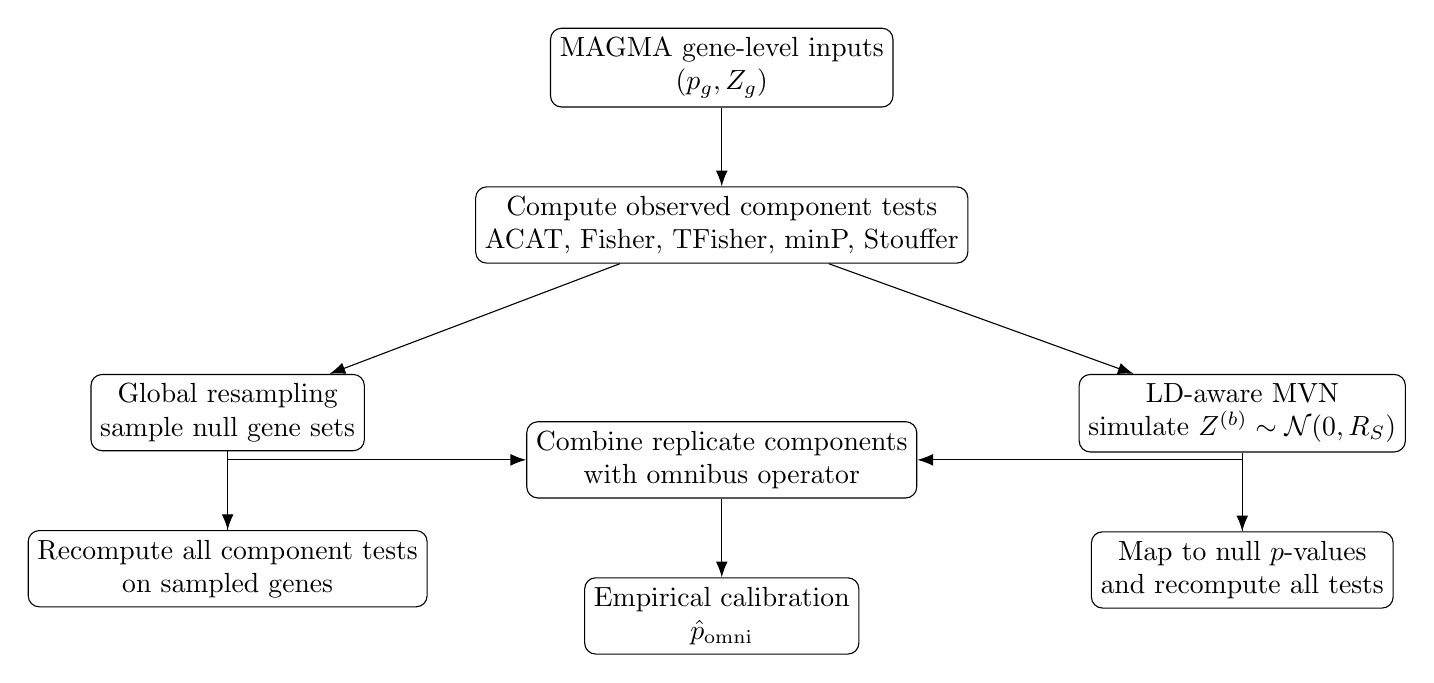
\begin{tikzpicture}[
node distance=10mm and 8mm,
box/.style={rectangle, rounded corners, draw, align=center, minimum width=33mm, minimum height=9mm},
line/.style={-{Latex[length=2mm]}}
]

\node[box] (input) {MAGMA gene-level inputs\\ $(p_g, Z_g)$};
\node[box, below=of input] (comp) {Compute observed component tests\\ ACAT, Fisher, TFisher, minP, Stouffer};
\node[box, below left=14mm and 14mm of comp] (global) {Global resampling\\ sample null gene sets};
\node[box, below right=14mm and 14mm of comp] (mvn) {LD-aware MVN\\ simulate $Z^{(b)}\sim\mathcal{N}(0,R_S)$};
\node[box, below=of global] (global2) {Recompute all component tests\\ on sampled genes};
\node[box, below=of mvn] (mvn2) {Map to null $p$-values\\ and recompute all tests};
\node[box, below=20mm of comp] (omni) {Combine replicate components\\ with omnibus operator};
\node[box, below=of omni] (cal) {Empirical calibration\\ $\hat p_{\mathrm{omni}}$};

\draw[line] (input) -- (comp);
\draw[line] (comp) -- (global);
\draw[line] (comp) -- (mvn);
\draw[line] (global) -- (global2);
\draw[line] (mvn) -- (mvn2);
\draw[line] (global2) |- (omni);
\draw[line] (mvn2) |- (omni);
\draw[line] (omni) -- (cal);

\end{tikzpicture}
\caption{Schematic overview of CATFISH null calibration strategies.}
\label{fig:catfish_workflow}
\end{figure*}

\subsection{Gene-level inputs from MAGMA}

Genome-wide association study (GWAS) summary statistics were aggregated into gene-level association metrics using MAGMA’s LD-aware SNP-wise gene model, employing an external reference panel to characterize local LD structure. SNPs were mapped to genes based on gene boundaries, optionally extended by flanking regions, resulting in per-gene outputs that included a gene-level $p$-value, $p_g$, and an association-strength $Z$ statistic, $Z_g$. To mitigate residual confounding attributable to gene length and SNP density, gene-level $Z$ statistics were optionally regressed on $\log(L_g)$ and $\log(S_g)$, where $L_g$ denotes gene length and $S_g$ the number of mapped SNPs. The residuals from this regression were then transformed back into adjusted gene-level $p$-values. The adjusted gene-level association evidence was subsequently used as input to CATFISH.

\subsection{Component pathway tests}

Each pathway in CATFISH is evaluated using a panel of complementary component tests, comprising ACAT, Fisher’s method, adaptive soft TFisher, minP, and Stouffer’s method. This collection of tests is deliberately heterogeneous because each procedure exhibits maximal sensitivity under a distinct pathway signal architecture. Specifically, ACAT and minP are most powerful for sparse architectures dominated by one or a small number of highly significant genes, whereas Fisher’s and Stouffer’s methods are better suited to detecting diffuse enrichment patterns involving many moderately associated genes. The adaptive soft TFisher test provides an intermediate, tail-adaptive compromise between these extremes. Formal mathematical definitions of all component statistics are given in Appendix~A.

\subsection{Dependence structure and motivation for null calibration}

A central feature of CATFISH is that its component tests are not statistically independent. First, they are deterministically coupled because each component test statistic is derived from the same within-pathway, gene-level evidence, typically $\{p_g\}_{g \in S}$ and, in some cases, $\{Z_g\}_{g \in S}$. As a result, even under the hypothetical scenario in which gene-level test statistics are mutually independent, the corresponding component $p$-values would nonetheless be correlated, since they represent distinct transformations of a common underlying signal. For instance, both Fisher’s method and soft TFisher are primarily sensitive to an enrichment of moderately small gene-level $p$-values; Stouffer’s method is driven by coherent shifts in gene-level $Z$-scores, and ACAT and minP tend to yield extreme values when one or a small number of genes exhibit exceptionally small $p$-values.

Second, gene-level inputs within a pathway are themselves frequently correlated as a consequence of LD, overlapping SNP annotations, shared local genomic architecture, and broader polygenic background effects. These factors induce additional dependence among gene-level $p$-values and $Z$-scores and, in turn, further strengthen dependence among the resulting pathway-level component tests. Post hoc selection across methods, for example, by taking the minimum $p$-value across component tests or by adaptively tuning TFisher thresholds, introduces an additional layer of dependence. Consequently, naive cross-method combination procedures that assume independence may be statistically miscalibrated and can become anti-conservative.

To address this, CATFISH interprets analytically derived omnibus statistics that aggregate across methods as descriptive summaries and derives final inferential conclusions using a null calibration procedure that explicitly preserves dependence. CATFISH provides two such dependence-aware null calibration strategies. The primary inferential approach is LD-aware multivariate normal (MVN) calibration, which, by construction, preserves pathway-specific gene–gene dependence as well as cross-method dependence. MAGMA gene-set analysis is explicitly built on the idea that genes are dependent due to LD, and it addresses this by modeling gene-level residuals as multivariate normal with correlation set to a gene–gene correlation matrix computed during gene analysis. This provides a principled motivation for using an MVN-based null generator when you subsequently apply alternative gene-set statistics to MAGMA gene outputs. In addition, CATFISH offers a global gene-set resampling mode, which maintains the empirical genome-wide distribution of gene-level test statistics and cross-method dependence, but does not explicitly retain the within-pathway LD structure. As the MVN-based approach more directly captures pathway-specific dependence, we recommend it as the default calibration strategy, while presenting the global resampling approach in Appendix A as an auxiliary option.



\subsection{LD-aware MVN omnibus calibration}

To account simultaneously for correlation among genes within a pathway and dependence among the component pathway tests, CATFISH calibrates the final omnibus statistic under a pathway-specific multivariate normal (MVN) null. For a pathway $S=\{g_1,\dots,g_d\}$, let $R_S$ denote the corresponding gene--gene correlation matrix, typically obtained from MAGMA-derived gene-correlation estimates. Under the LD-aware null, CATFISH generates replicate null gene-level score vectors as
\[
Z^{(b)} \sim \mathcal{N}(0, R_S), \qquad b=1,\dots,B.
\]

For $p$-based component statistics, null gene-level $p$-values are obtained from the same latent MVN draw via a Gaussian-copula mapping. Under the default two-sided convention,
\[
U_g^{(b)}=\Phi\!\left(Z_g^{(b)}\right),
\qquad
p_g^{(b)} = 2\min\{U_g^{(b)},\,1-U_g^{(b)}\},
\]
where $\Phi(\cdot)$ denotes the standard normal cumulative distribution function. This ensures that both $Z$-based and $p$-based component tests are recomputed from a common dependence-preserving null realization.

For each replicate, CATFISH recomputes all component pathway tests from the same simulated pathway and forms the replicate component vector
\[
\mathbf{p}^{(b)}(S)
=
\Big(
p_{\mathrm{ACAT}}^{(b)}(S),\,
p_{\mathrm{Fisher}}^{(b)}(S),\,
p_{\mathrm{TFisher}}^{(b)}(S),\,
p_{\mathrm{Stouffer}}^{(b)}(S),\,
p_{\mathrm{minP}}^{(b)}(S)
\Big),
\]
with the observed component vector $\mathbf{p}^{\mathrm{obs}}(S)$ defined analogously from the real data. CATFISH then applies a prespecified omnibus operator $\mathcal{O}(\cdot)$, such as ACAT across methods or a minP-type across-method operator, to obtain
\[
p_{\mathrm{omni}}^{(b)}(S)=\mathcal{O}\!\left(\mathbf{p}^{(b)}(S)\right),
\qquad
p_{\mathrm{omni}}^{\mathrm{obs}}(S)=\mathcal{O}\!\left(\mathbf{p}^{\mathrm{obs}}(S)\right).
\]

The final MVN-calibrated omnibus $p$-value is estimated empirically as
\[
\hat p_{\mathrm{omni,mvn}}(S)
=
\frac{
1+\sum_{b=1}^{B}\mathbf{1}\!\left(
p_{\mathrm{omni}}^{(b)}(S)\le p_{\mathrm{omni}}^{\mathrm{obs}}(S)
\right)
}{
B+1
}.
\]

This calibration targets the null distribution of the complete pathway-analysis procedure rather than the marginal null distribution of each component test considered in isolation. Because all component statistics are recomputed from the same simulated pathway in each replicate, the MVN procedure preserves both within-pathway gene dependence and cross-method dependence by construction. In practice, CATFISH fixes the pathway-specific correlation matrix $R_S$ and repeatedly simulates correlated null gene-score vectors from this matrix; details on construction, stabilization, and factorization of $R_S$ are provided in Appendix~A.

In addition to this LD-aware MVN approach, CATFISH also supports global gene-set resampling as a secondary calibration mode. However, MVN calibration is the recommended inferential procedure because it directly preserves pathway-specific dependence structure induced by LD while calibrating the final omnibus statistic under the full analysis pipeline.






\begin{algorithm}[htbp]
\caption{LD-aware MVN calibration for pathway $S$}
\label{alg:mvn_calibration}
\begin{algorithmic}[1]
\Require Pathway $S=\{g_1,\dots,g_d\}$, pairwise gene-correlation input, number of replicates $B$, omnibus operator $f_{\mathrm{omni}}$
\Ensure Calibrated omnibus $p$-value $\hat p_{\mathrm{omni,mvn}}(S)$

\State Construct the pathway-specific correlation matrix $R_S$
\State Set diagonal entries to 1
\State Fill off-diagonal entries with available pairwise correlations $r_{ij}$
\State Set missing pairs to 0
\State Clip extreme correlations if needed (e.g.\ $|r_{ij}|\le 0.999$)
\State Enforce positive-definiteness of $R_S$ if needed

\State Compute the observed component pathway $p$-values for $S$
\State Compute the observed omnibus value
\[
p_{\mathrm{omni}}^{\mathrm{obs}}(S)
=
f_{\mathrm{omni}}\!\left(\{p_j^{\mathrm{obs}}(S)\}\right)
\]

\For{$b=1,\dots,B$}
    \State Simulate correlated null gene-level scores
    \[
    Z^{(b)} \sim \mathcal{N}(0,R_S)
    \]
    \State Map the same latent draw to null gene-level $p$-values using a Gaussian copula
    \[
    U_g^{(b)}=\Phi\!\left(Z_g^{(b)}\right),
    \qquad
    p_g^{(b)} = 2\min\{U_g^{(b)},\,1-U_g^{(b)}\}
    \]
    \State Recompute all $p$-based component tests from $\{p_g^{(b)}\}$
    \State Recompute Stouffer from $\{Z_g^{(b)}\}$
    \State Combine replicate component $p$-values using the same omnibus rule:
    \[
    p_{\mathrm{omni}}^{(b)}(S)
    =
    f_{\mathrm{omni}}\!\left(\{p_j^{(b)}(S)\}\right)
    \]
\EndFor

\State Estimate the calibrated omnibus $p$-value as
\[
\hat p_{\mathrm{omni,mvn}}(S)
=
\frac{
1+\sum_{b=1}^{B}\mathbf{1}\!\left(
p_{\mathrm{omni}}^{(b)}(S)\le p_{\mathrm{omni}}^{\mathrm{obs}}(S)
\right)
}{
B+1
}
\]

\State \Return $\hat p_{\mathrm{omni,mvn}}(S)$
\end{algorithmic}
\end{algorithm}


\subsection{Omnibus pathway combination across methods}

Let
\[
\mathcal{P}(S)=
\left\{
p_{\mathrm{ACAT}}(S),\,
p_{\mathrm{Fisher}}(S),\,
p_{\mathrm{TFisher}}(S),\,
p_{\mathrm{minP}}(S),\,
p_{\mathrm{Stouffer}}(S)
\right\}
\]
denote the available component pathway $p$-values for pathway $S$, with $K=|\mathcal{P}(S)| \le 5$. CATFISH provides two omnibus summary statistics: (i) ACAT-O, which aggregates method-specific $p$-values via a Cauchy-based transformation, and (ii) minP-O, which is defined as the minimum $p$-value across methods and is calibrated using an analytic mapping that assumes independence. As the component tests are dependent, these analytic omnibus values are mainly useful for descriptive ranking, whereas the primary inferential measure is the dependence-calibrated omnibus \$p\$-value obtained from the MVN procedure above.

\subsection{Multiple testing correction}

Across all pathways, final omnibus $p$-values were adjusted using the Benjamini--Hochberg FDR procedure. As each pathway yields a single final omnibus \$p\$-value, no additional penalty is needed for the number of component tests, since the dependence-aware calibration already accounts for the post hoc best-of-tests behavior.

\subsection{Candidate-gene prioritization}

To prioritize genes beyond top-SNP, MAGMA, or top-pathway evidence alone, we integrated support across these three complementary layers. For each gene, we summarized multi-layer support using a support-count plus strength score that gives primary weight to agreement across layers and secondary weight to continuous evidence strength within each layer. Genes supported by at least two layers were prioritized for downstream interpretation. The exact scoring rule is given in Appendix~B.

\section{Results and discussion}




\subsection{Null calibration of CATFISH pathway tests}

To assess the null calibration of CATFISH, we simulated gene-level $Z$-scores from a MVN distribution under three LD settings: (i) LD\_independent ($\rho = 0$), (ii) LD\_moderate ($\rho = 0.3$), and (iii) LD\_strong ($\rho = 0.7$), and three pathway sizes ($m = 5, 25, 50$ genes). These scenarios characterize the behavior of the CATFISH component tests and the omnibus statistic as within-pathway gene correlations increase from none to strong, with the pathway correlation matrix specifying the dependence structure among gene-level test statistics and serving as a proxy for within-pathway LD. For each simulated pathway, we applied the five component tests (ACAT, Fisher's method, adaptive soft TFisher, minP, and Stouffer's method) and combined their $p$-values into a single omnibus statistic using ACAT. Under the null, calibration was evaluated using the genomic inflation factor ($\lambda$) and the empirical type I error rate at $\alpha = 0.05$. We compared two strategies for estimating pathway-level significance: (i) an analytic procedure that assumes genes within a pathway are independent (red), and (ii) MVN calibration procedure (blue), which resampled null $Z$-scores from the pathway’s correlation matrix modeling LD.

Under LD\_independent, the analytic and MVN results agreed across pathway sizes, as expected when genes are effectively uncorrelated. Under LD\_moderate and especially LD\_strong, several analytic tests were clearly miscalibrated. In Fig.~2A, this appears as $\lambda$ values deviating from 1, and in Fig.~2B, as empirical type I error rates differing from the nominal 0.05. Depending on the method, ignoring LD produced either inflated or overly conservative tests. Thus, neglecting within-pathway dependence caused method-specific calibration distortions rather than uniformly anti-conservative behavior.

This pattern reflects the known sensitivity of many $p$-value combination methods to dependence among input statistics, especially when their null distributions assume independence. Here, $\lambda < 1$ does not imply inflation of the test statistic; instead, it indicates a conservative test, with null $p$-values stochastically larger than expected and conventional significance thresholds harder to reach. MVN calibration largely alleviated these problems. Across linkage disequilibrium (LD) structures and pathway sizes, MVN-calibrated component tests closely matched the expected null distribution, with $\lambda \approx 1$ and type I error rates near the nominal 0.05 level (Fig.~2A,B). The omnibus statistic showed similar improvement. Among analytic methods, ACAT was relatively more stable, consistent with its reported robustness to dependence, but MVN calibration still provided the most uniform and reliable control for both individual component tests and the omnibus statistic.



\begin{figure*}[!t]
    \centering
    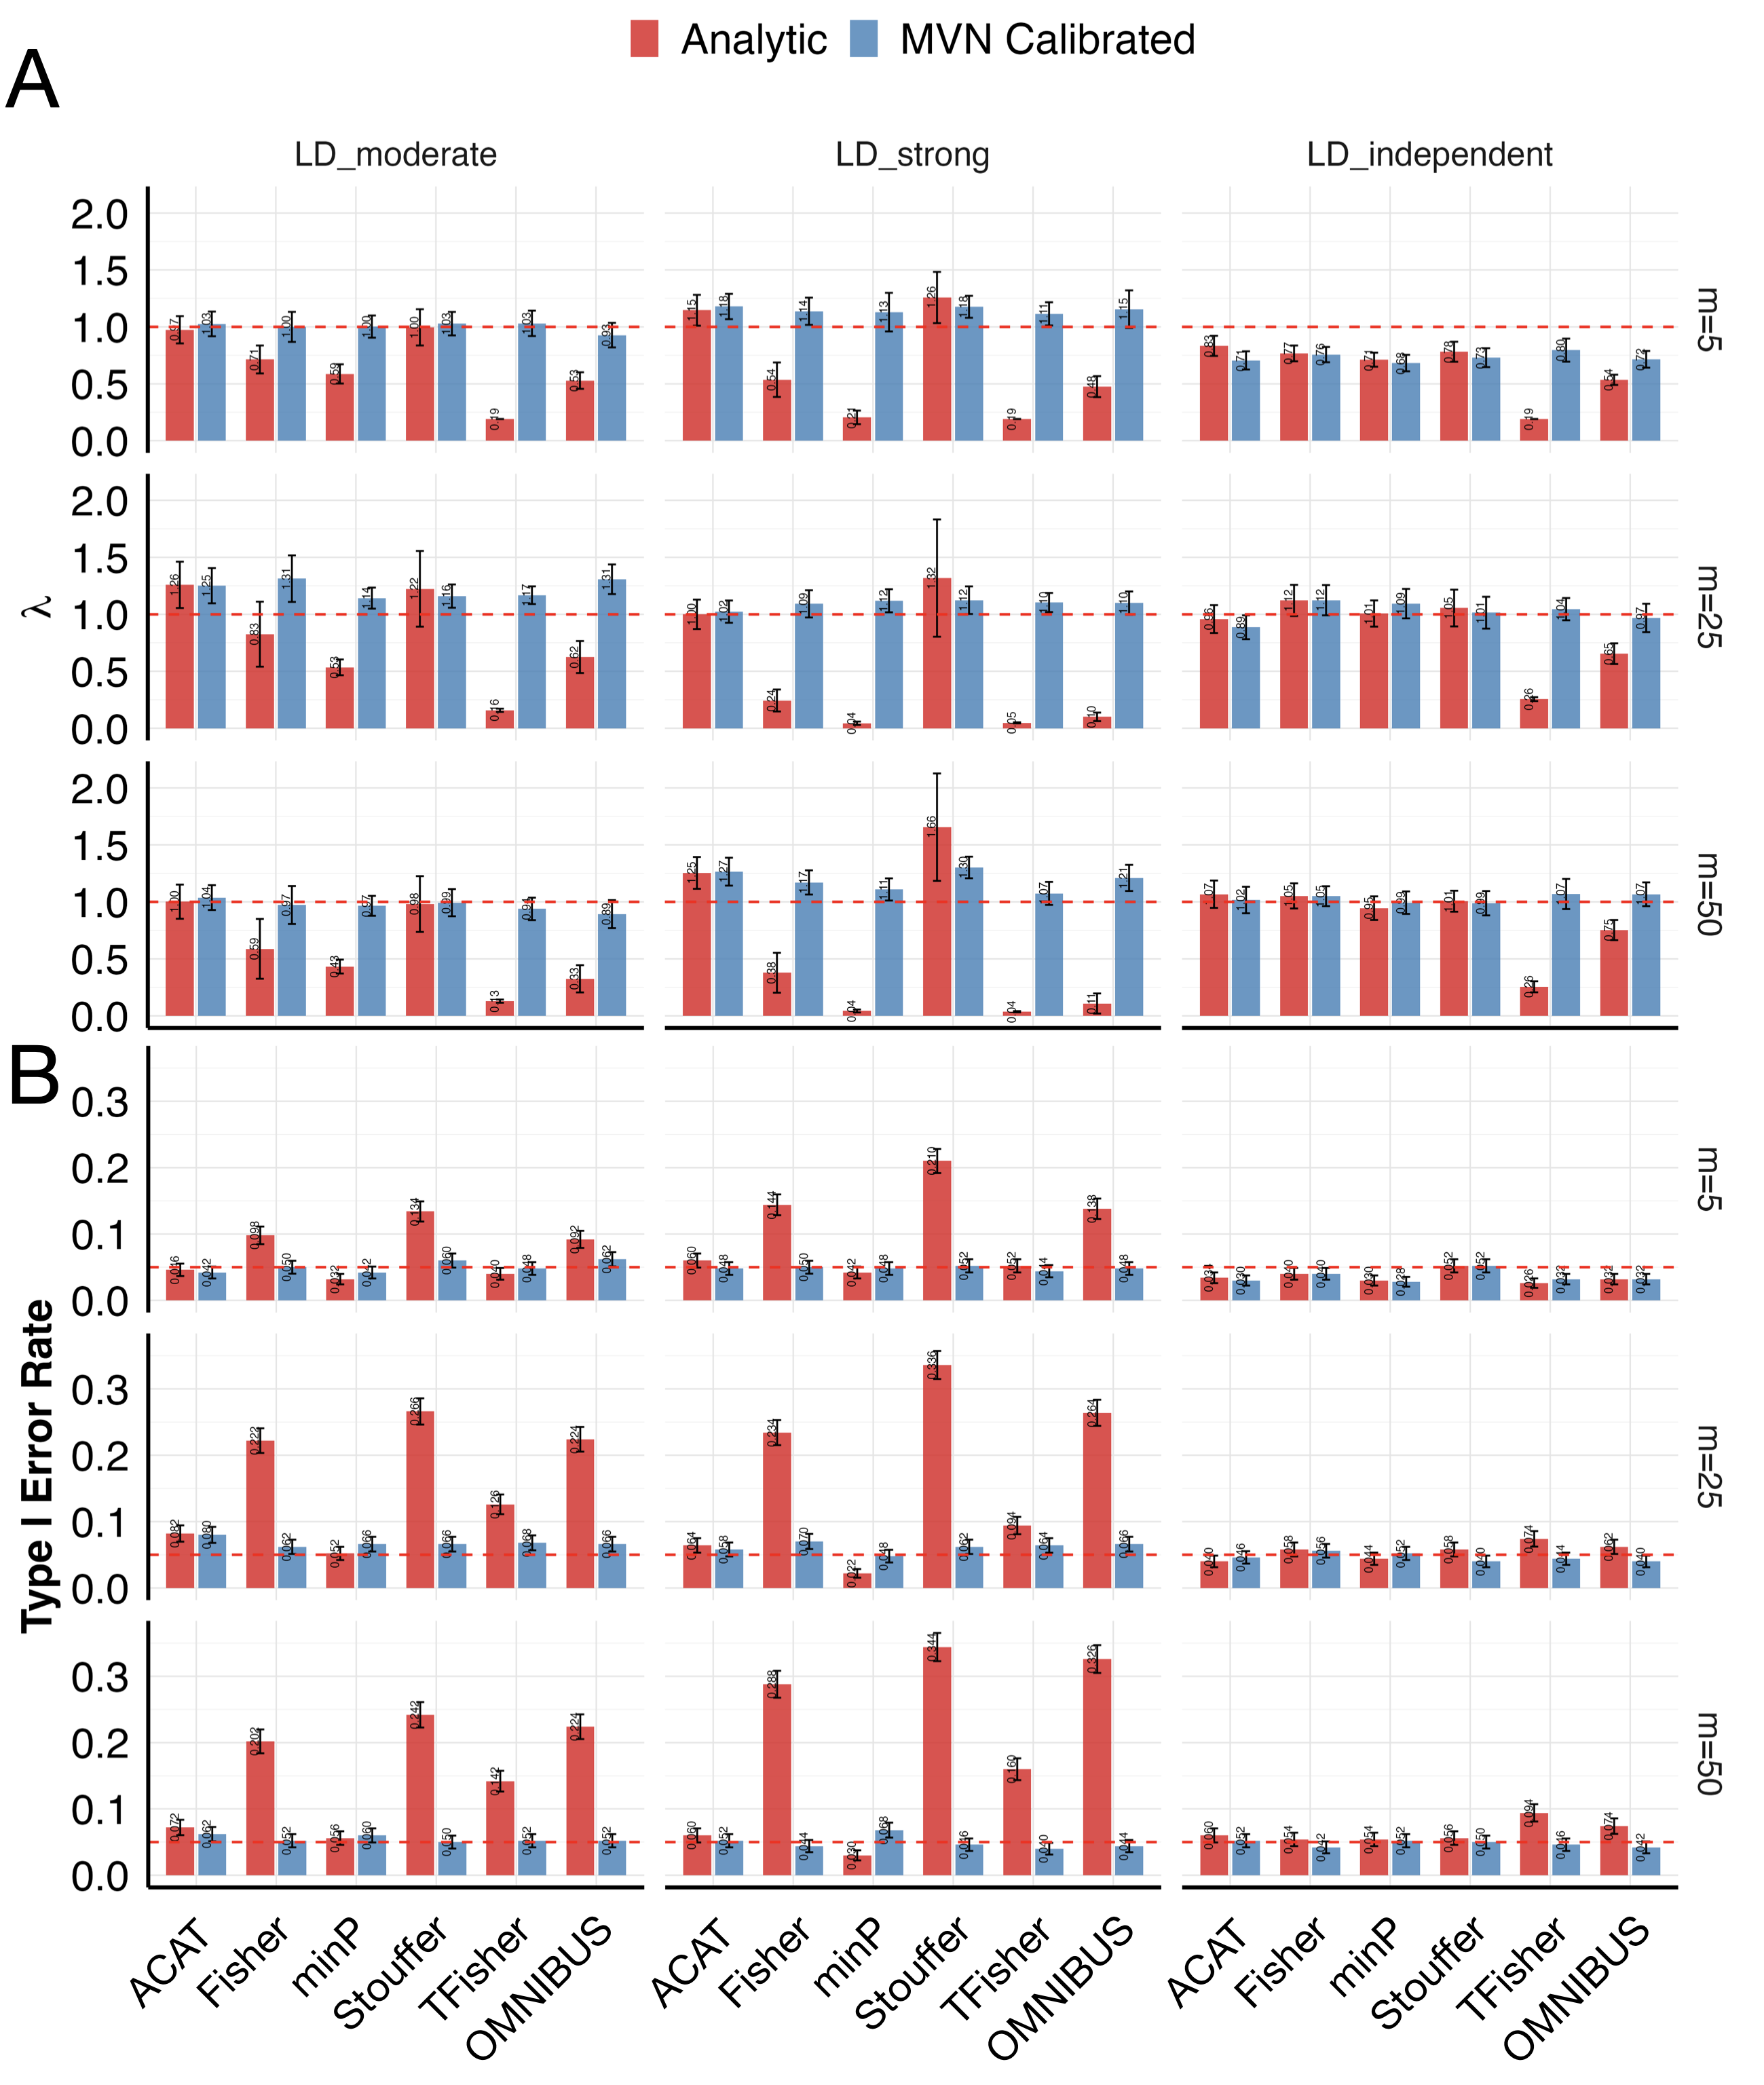
\includegraphics[width=\textwidth]{Figures/Fig2.Simulation_validation/Fig2.Null_Calibration_and_Genomic_Control_Across_LD_Regimes.png}
    \caption{\small \textbf{Null calibration and genomic control across LD regimes.}
    Pathway-level $p$-values were evaluated under the global null using simulated gene-level $Z$-scores across three within-pathway LD regimes (LD\_moderate, LD\_strong, LD\_independent) and pathway sizes ($m=5, 25, 50$). \textbf{A.} Genomic control inflation factor ($\lambda$) for each component test (ACAT, Fisher, minP, Stouffer, TFisher) and the omnibus, comparing analytic independence-based calculations (red) with LD-aware MVN calibration (blue). The dashed line indicates the nominal expectation ($\lambda=1$). Under moderate and strong LD, analytic $p$-values are frequently miscalibrated, whereas MVN calibration stabilizes $\lambda$ near 1 across methods and pathway sizes. Under LD independence, analytic and MVN results are broadly concordant. \textbf{B.} Empirical type I error at $\alpha=0.05$ for the same settings. Analytic $p$-values show inflated or unstable false-positive rates under LD, whereas MVN calibration restores near-nominal error control. Error bars indicate sampling variability across null replicates.}
    \label{fig:null_calibration_ld}
\end{figure*}


\subsection{Stress testing omnibus robustness under component misspecification}

To evaluate the robustness of the CATFISH omnibus to component-level misspecification, we conducted a structured component-breakage stress test under the global null. For each simulated pathway, gene-level $Z$-scores were generated from a multivariate normal distribution under three LD regimes (LD\_independent, LD\_moderate, LD\_strong) and three pathway sizes ($m = 5, 25, 50$). We then computed the five CATFISH component tests—ACAT, Fisher’s method, adaptive soft TFisher, minP, and Stouffer’s method—and introduced controlled misspecification by designating $k = 1,2,3,4$ of the five components as ``broken''. For each value of $k$, results were averaged across all possible combinations of broken components so that the summary reflects the general impact of increasing component corruption rather than the behavior of any single configuration.

A key feature of this stress test is that the omnibus statistic was not evaluated against a clean null. Instead, after breaking the selected components in the observed data, the omnibus statistic was recomputed and recalibrated using a matching broken MVN null. Specifically, null replicates were generated under the same LD structure and subjected to the identical component-breakage pattern before constructing the omnibus null distribution. This design isolates a central question: whether MVN-based recalibration can preserve valid inference even when some component tests are misspecified. Calibration was evaluated using two complementary diagnostics: genomic control inflation ($\lambda$, with nominal expectation $\lambda = 1$) and empirical type I error at $\alpha = 0.05$. Error bars represent standard errors obtained from simulation replicates.

The dominant pattern across both panels is that the MVN-recalibrated omnibus remains substantially more stable than the individual component tests as the number of broken components increases. In the type I error analysis, the black curve corresponding to Omnibus (MVN) stays close to the nominal 0.05 reference across LD regimes, pathway sizes, and breakage levels, which is the central result of the stress test. In contrast, several individual component tests deteriorate monotonically as additional components are broken, with false-positive rates drifting upward, often markedly under nontrivial LD. This behavior is most pronounced for Stouffer and Fisher, which become increasingly anti-conservative under LD\_moderate and especially LD\_strong, with the deviation further amplified at larger pathway sizes. ACAT also degrades under breakage, although typically less severely than Stouffer. By contrast, TFisher and minP often show more conservative median behavior in the $\lambda$ panel, particularly under stronger LD, although such conservatism does not necessarily imply proper control of tail error.

The $\lambda$ panel provides a complementary perspective. As the number of broken components increases, the individual component tests often drift away from the nominal expectation of $\lambda = 1$, but the direction of departure depends on the method. Some become clearly inflated ($\lambda > 1$), whereas others become strongly conservative ($\lambda < 1$). Importantly, the omnibus (MVN) does not mirror these large excursions. Instead, its $\lambda$ values remain comparatively flat as $k$ increases, indicating that the recalibrated omnibus is resistant to the accumulation of instability from multiple misspecified inputs. In some settings the omnibus is mildly conservative rather than exactly centered at 1, particularly under stronger LD, but this departure is modest relative to the pronounced deviations observed for several broken component tests and is accompanied by substantially improved type I error control.

An important nuance emerges when $\lambda$ and empirical type I error are considered jointly. For example, TFisher can exhibit $\lambda$ values well below 1 in some panels, suggesting conservative median behavior, yet still show non-nominal type I error. This highlights that $\lambda$ is a median-based summary and does not, on its own, guarantee correct tail calibration. The converse is also possible: a method may have $\lambda$ numerically close to 1 while still exhibiting inflated false positives if its tail behavior is poorly controlled. By this stricter criterion, the recalibrated omnibus is the most consistent performer in the figure.By this stricter standard, the recalibrated omnibus is the most robust and consistently well-calibrated procedure in the figure.

This stress test demonstrates that explicit MVN recalibration protects the omnibus against progressive degradation of its component tests. That is the central practical message. The individual methods respond differently to misspecification because they embody different aggregation mechanisms and therefore fail in different ways: Stouffer is particularly sensitive to coherent directional distortion, Fisher is sensitive to systematic compression of moderate $p$-values, and ACAT, although often viewed as relatively robust, still accumulates excess false positives when enough corrupted inputs are introduced. The omnibus does not remove misspecification at the component level; rather, when recalibrated against a matching LD-aware null, it substantially buffers these distortions and preserves overall null control.

The figure also shows that robustness should be judged primarily by empirical type I error rather than by $\lambda$ alone. Some component tests appear conservative in terms of $\lambda$ while simultaneously exhibiting unacceptable false-positive behavior, which would be easy to misinterpret if $\lambda$ were considered in isolation. In contrast, the omnibus (MVN) remains close to the nominal type I error threshold across breakage levels, LD conditions, and pathway sizes, while showing only modest movement in $\lambda$. This represents a stronger and more defensible notion of robustness than simply asking whether $\lambda$ is numerically closest to 1 in every panel.

The broader implication is methodological. If pathway inference is constructed from multiple component tests, then misspecification of some subset of those tests is a realistic scenario rather than an exceptional one. A useful omnibus should therefore not depend on every component being analytically well calibrated. These results indicate that the combination step is reliable only when paired with LD-aware null recalibration, and that the CATFISH omnibus remains usable even when multiple constituent tests are degraded. Put differently, the stability of the omnibus in this setting is not an intrinsic property of ACAT alone; it arises from combining evidence and then recalibrating the resulting statistic under the appropriate broken, LD-aware null. This is why the black curve remains comparatively flat while several component-specific curves drift strongly away from nominal behavior.



\begin{figure*}[!t]
    \centering
    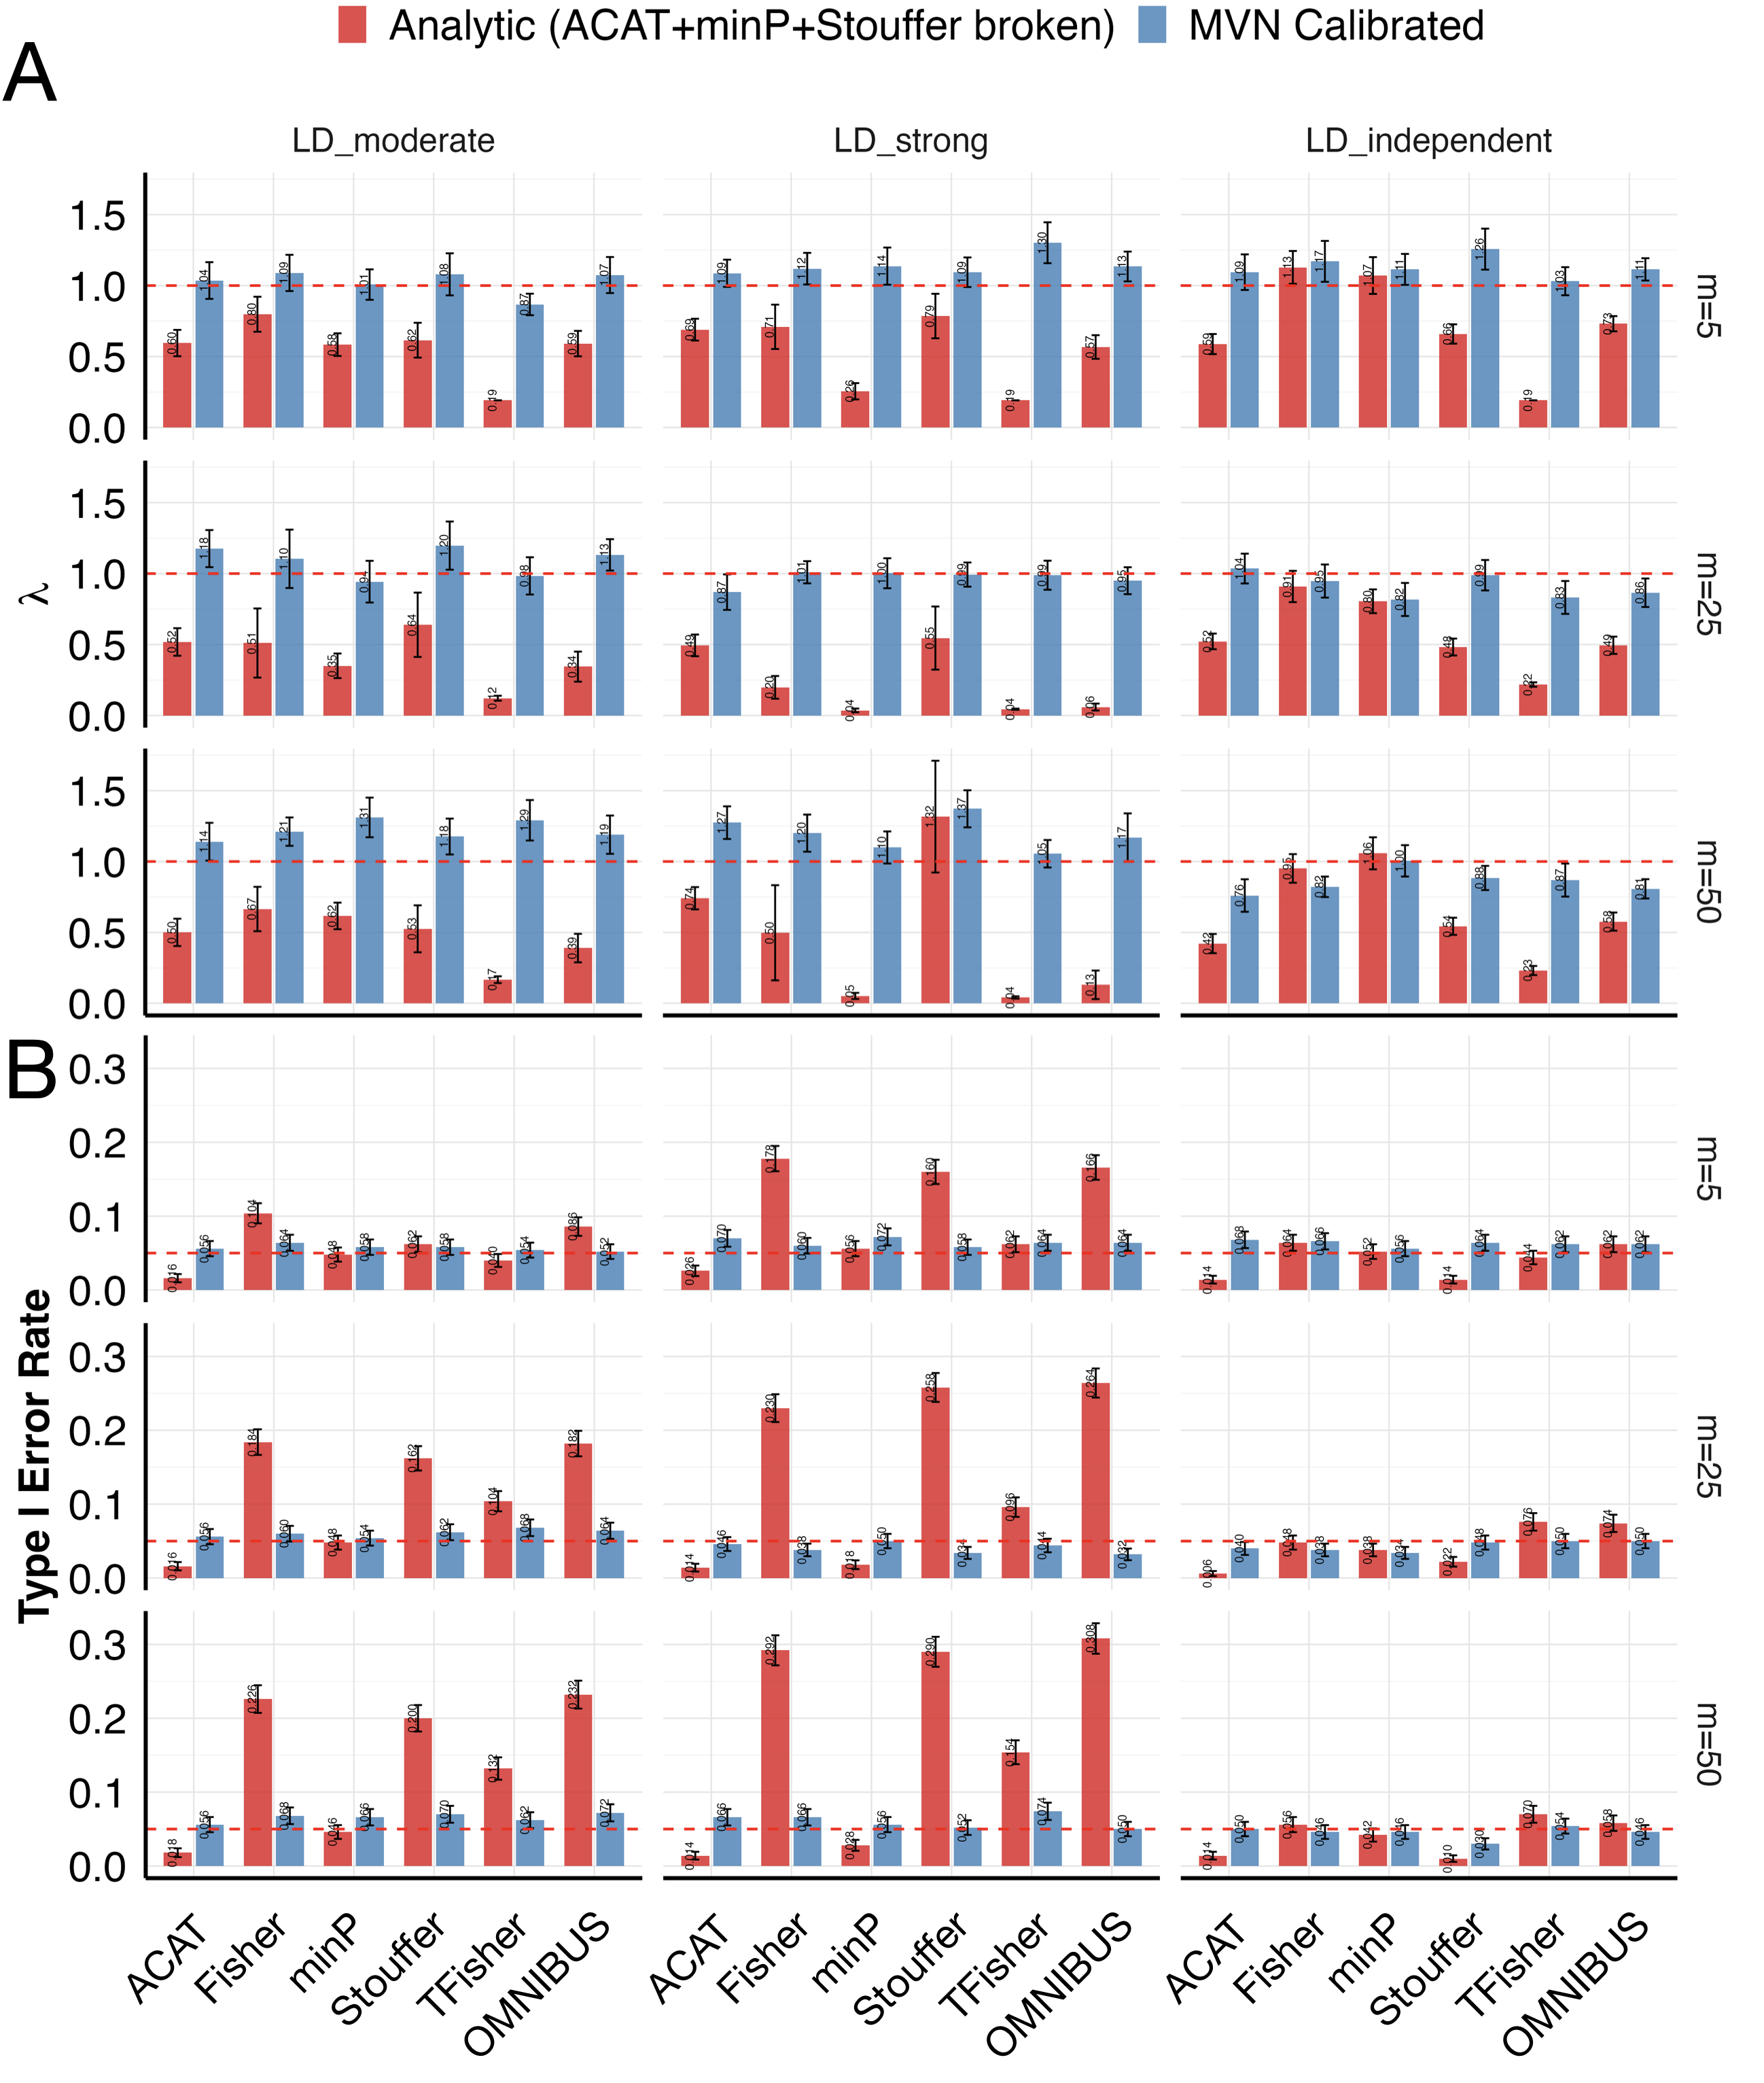
\includegraphics[width=\textwidth]{Figures/SuppFig/SuppFig1.Stress_test_for_null_calibration_and_genomic_control.png}
    \caption{\textbf{Stress test for null calibration and genomic control.}
    \textbf{A.} To stress-test robustness to component miscalibration, we repeated null simulations across LD regimes and pathway sizes but intentionally computed a subset of component $p$-values using an analytic procedure that ignores LD (red; ``broken''), while the MVN-calibrated pipeline uses the correct LD-aware null (blue). The resulting $\lambda$ values illustrate that LD-ignorant component calculations can induce substantial miscalibration that propagates into the omnibus, whereas MVN calibration keeps $\lambda$ near 1 across conditions.
    \textbf{B.} Empirical type I error rates at $\alpha = 0.05$ are shown for the same stress-test conditions. LD-ignorant analytic components lead to marked inflation in false positives in LD\_moderate/LD\_strong settings, while MVN calibration maintains approximately nominal type I error across pathway sizes and LD regimes. Error bars indicate sampling variability across null replicates.}
\end{figure*}


\subsection{Power under heterogeneous pathway architectures}

We next evaluated statistical power under alternative signal architectures that varied in signal density and directional coherence. Signal density is the proportion of pathway genes that are truly associated with the phenotype (i.e., causal). Directional coherence is the extent to which effects of causal genes align in the same direction versus oppose each other. Thus, the simulations assessed not only how many genes were causal, but also how their effects were distributed and oriented across the pathway. To vary signal density, we modeled dense and sparse architectures. In dense architectures, a relatively large proportion of pathway genes was causal (about 30–50\%), and in sparse architectures, only a small proportion was causal (about 5–10\%). These scenarios contrast pathways where association signal is spread across many genes with those where it is concentrated in a small subset.

We also manipulated directional coherence. In these schemes, all causal genes had effects in the same direction, producing a consistent pathway-level association pattern. In the mixed-direction architecture, causal genes were split into positive and negative effects, with roughly half showing upward and half downward shifts. This represents pathways where relevant genes affect the phenotype but are not directionally aligned, a key scenario because methods that aggregate effects by direction can lose power when opposing effects partially cancel. Independently of signal density and directionality, we varied association strength at each causal gene by applying a mean shift, $\delta$, to simulated gene-level $Z$-scores. Larger $\delta$ values correspond to stronger per-gene effects and easier detection. We evaluated statistical power over a grid of $\delta$ values to compare methods under weak, moderate, and strong signal regimes.

Combining these elements, we defined five representative architectures: Dense\_Strong, Dense\_Weak, Mixed\_Direction, Sparse\_Moderate, and Sparse\_Strong (Table~1). Dense\_Strong models a pathway where many genes are causal, each with a strong signal; Dense\_Weak also assumes many causal genes but with weaker effects. Mixed\_Direction includes a moderate fraction of causal genes with effects of mixed sign. Sparse\_Moderate and Sparse\_Strong model pathways where only a small subset of genes is causal, with moderate and strong effects, respectively. Concordant effects could be uniformly positive or negative. For simplicity, we present the uniformly positive case without loss of generality.


\begin{figure*}[!t]
    \centering
    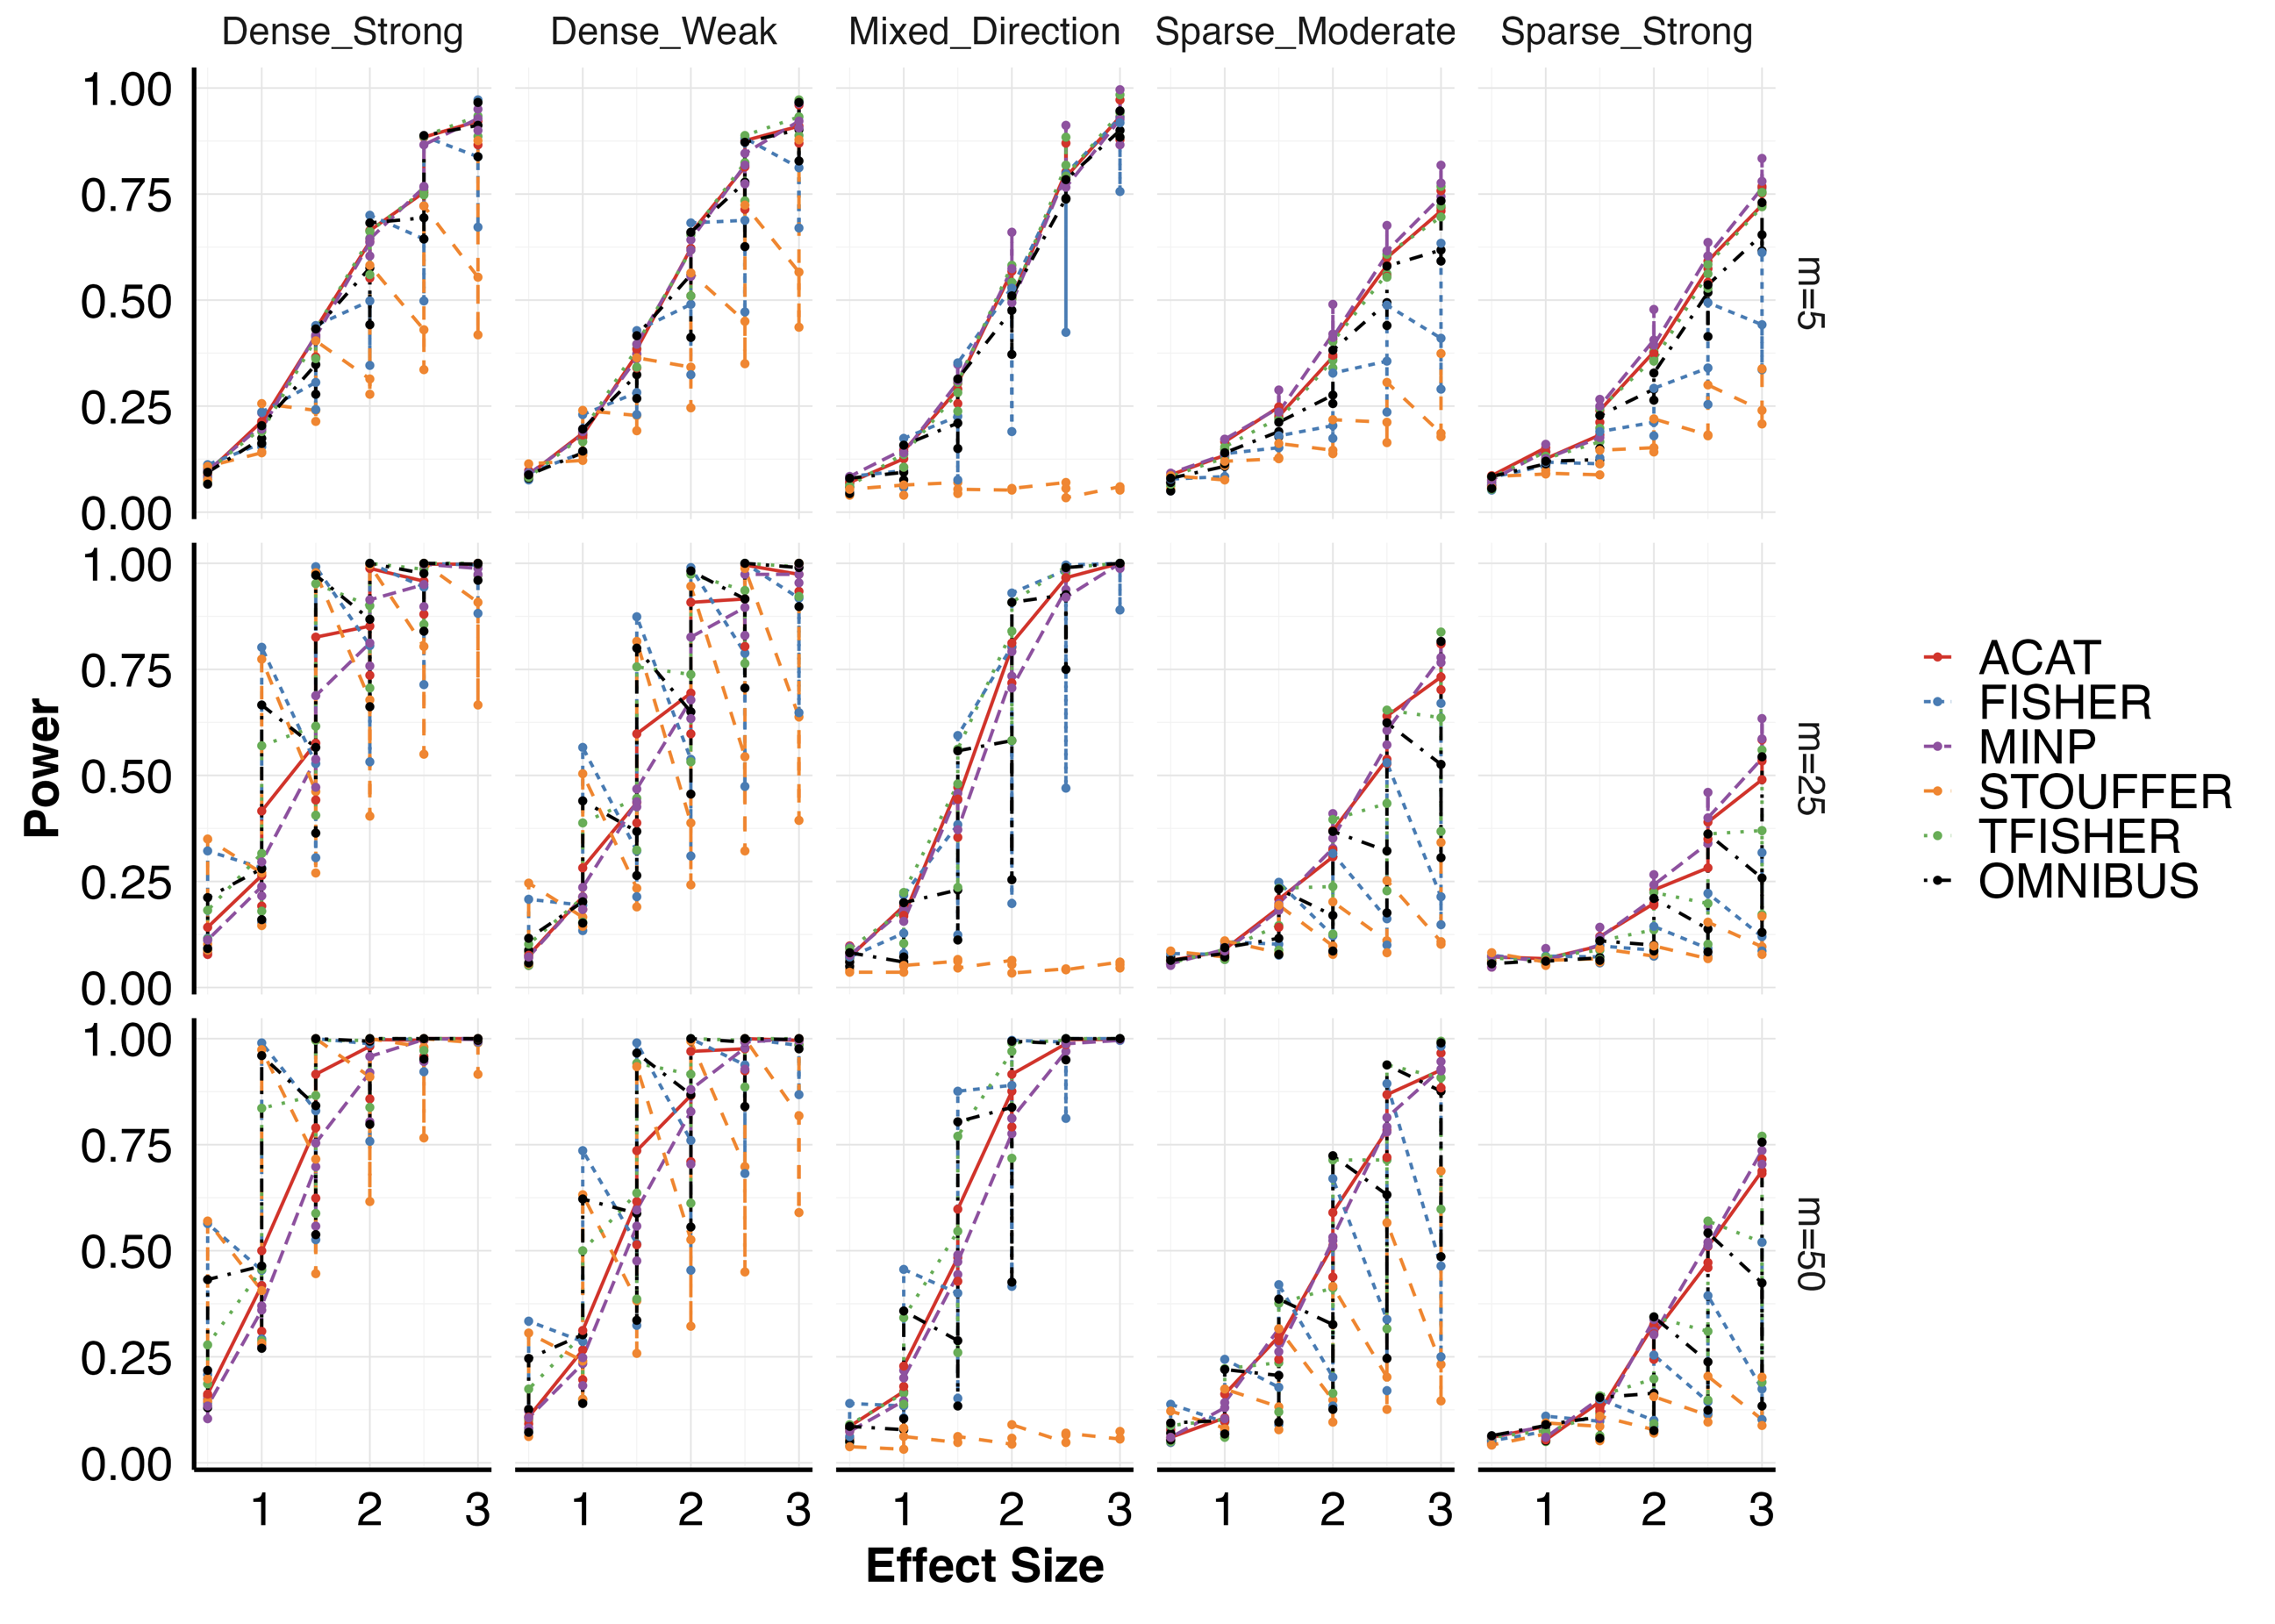
\includegraphics[width=\textwidth]{Figures/SuppFig/SuppFig2.Power_Under_Alternatives_and_MVN_Calibration.png}
    \caption{\textbf{Power under alternatives and MVN calibration.}
    Power was evaluated across five signal archetypes (Dense\_Strong, Dense\_Weak, Mixed\_Direction, Sparse\_Moderate, Sparse\_Strong), increasing effect sizes, and pathway sizes ($m = 5, 25, 50$), using MVN-calibrated $p$-values to ensure valid null control under LD. Curves compare individual component tests to the omnibus. Across signal shapes, no single component test uniformly dominates; rather, the best-performing component varies with sparsity, effect strength, and directionality. In contrast, the omnibus consistently tracks the upper envelope of component performance, providing robust power across heterogeneous alternatives while retaining valid calibration under the null.}
\end{figure*}


\begin{table*}[!t]
\centering
\caption{Signal architecture definitions used in power simulations.}
\begin{tabular}{llll}
\hline
Scenario label & Signal density (fraction causal) & Directional coherence & Per-gene effect magnitude \\
\hline
Dense\_Strong    & $\sim 0.50$ & Concordant (all $+$) & Swept over $\delta$ grid \\
Dense\_Weak      & $\sim 0.30$ & Concordant (all $+$) & Swept over $\delta$ grid \\
Mixed\_Direction & $\sim 0.30$ & Mixed ($+$ and $-$)  & Swept over $\delta$ grid \\
Sparse\_Moderate & $\sim 0.10$ & Concordant (all $+$) & Swept over $\delta$ grid \\
Sparse\_Strong   & $\sim 0.05$ & Concordant (all $+$) & Swept over $\delta$ grid \\
\hline
\end{tabular}
\end{table*}


\subsection{Robustness to incomplete LD information and adaptive component filtering}

To mimic practical settings where within-pathway gene–gene correlations are only partly available from LD-based estimates (e.g., MAGMA reports only some pairs), we evaluated omnibus calibration with a partially observed pathway correlation matrix (Fig.~3). Starting from a “true” correlation structure, we randomly removed a fraction of off-diagonal entries and compared three ways to generate omnibus null $p$-values: (i) an analytic fallback that assumes all genes are independent and ignores correlations (red), (ii) MVN calibration using the true correlation matrix (green), and (iii) MVN calibration using a matrix where missing correlations are set to zero (blue), mirroring our MAGMA-based correlation implementation (Fig.~3A). Across pathway sizes ($m = 5, 25, 50$) and missingness levels, the analytic fallback was strongly miscalibrated, with genomic control values far from the nominal $\lambda = 1$, showing that independence-based analytic approximations fail under LD. In contrast, MVN calibration stabilized the omnibus test, and the zero-imputed MVN approach consistently gave genomic control values closest to $\lambda \approx 1$ over a broad range of missingness (Fig.~3A), supporting zero-imputation when pairwise information is incomplete. Its advantage over MVN calibration with the fully observed matrix can arise in finite simulations because the positive-definite projection step shrinks and regularizes the correlation structure, improving conditioning and reducing Monte Carlo variability under the null.

\begin{figure*}[!t]
    \centering
    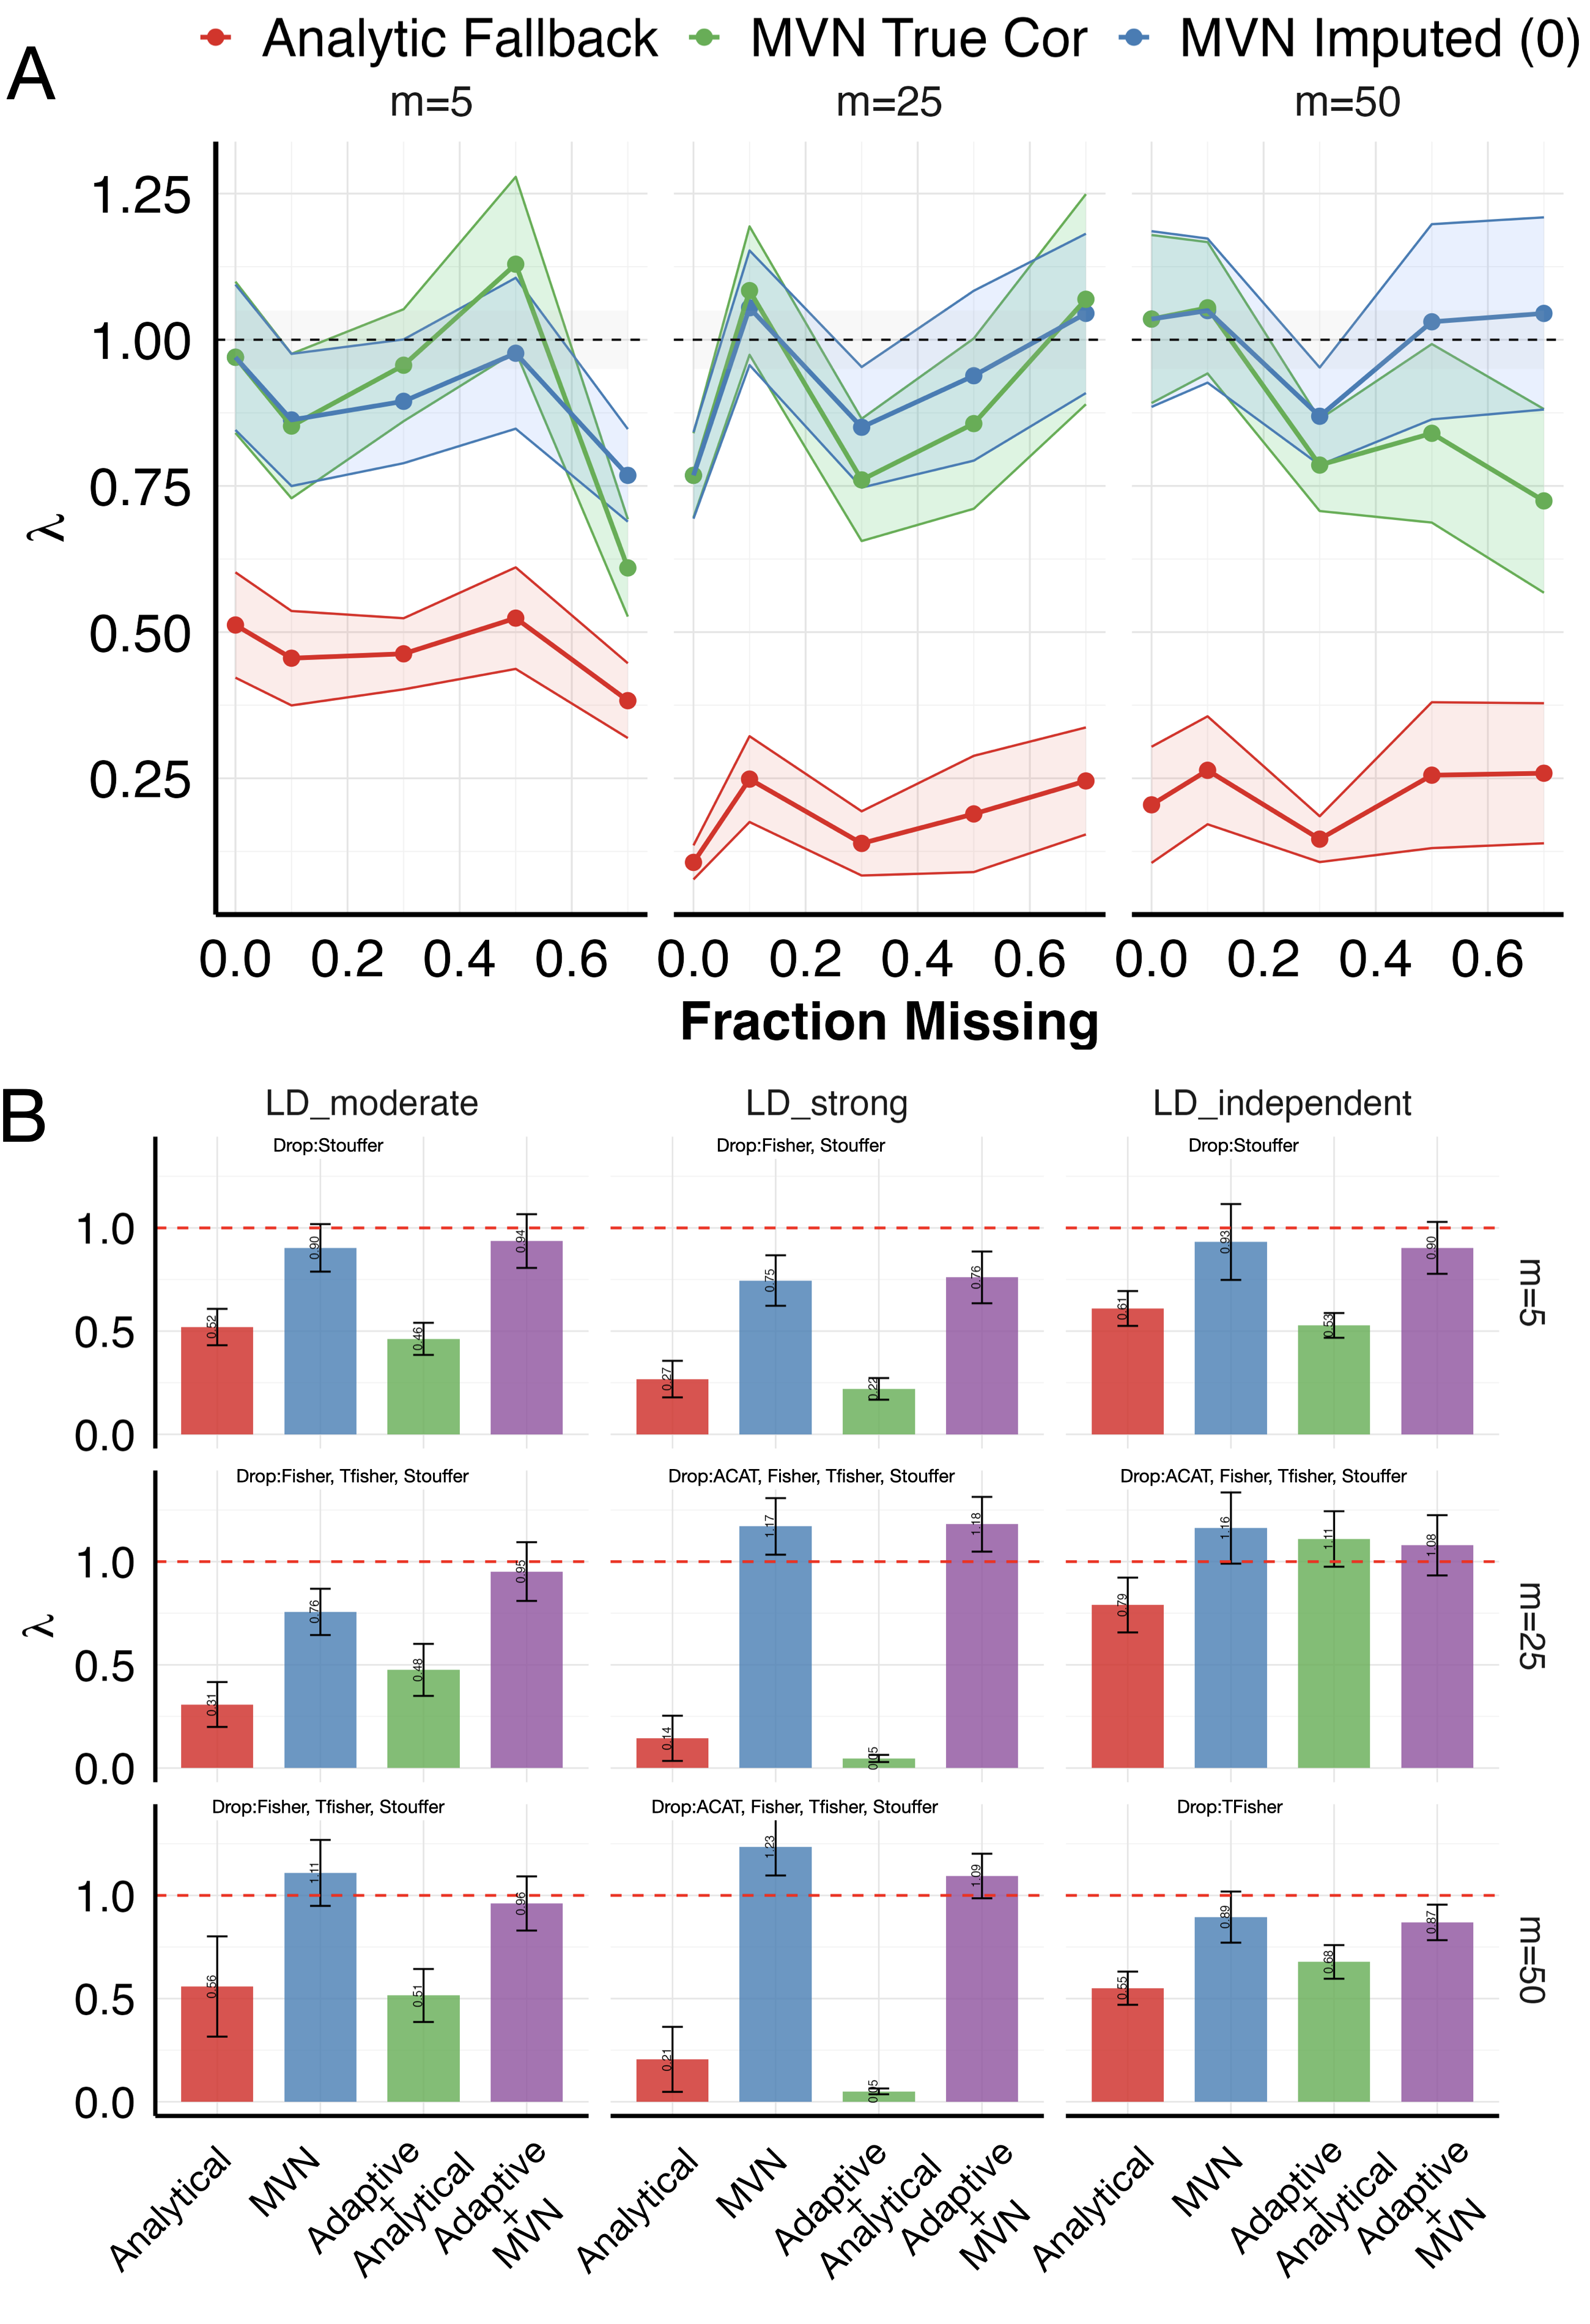
\includegraphics[width=\textwidth]{Figures/Fig3.Incomplete_Adaptive_OMNIBUS/Fig3.Genomic_Control_vs_Missing_Correlations.png}
    \caption{\textbf{Omnibus genomic control versus missing correlations.}
    \textbf{A.} We evaluated robustness of MVN-based omnibus calibration when the within-pathway gene--gene correlation matrix is only partially observed. Gene $Z$-scores were simulated under the null from a true correlation structure, and then a fraction of off-diagonal correlation entries was randomly removed to mimic incomplete MAGMA pairwise outputs. The omnibus genomic control factor ($\lambda$; dashed line indicates $\lambda = 1$) is shown as a function of the fraction missing for three strategies: an analytical omnibus that combines component tests without LD-aware calibration, an LD-aware MVN omnibus calibrated using MVN resampling, and an imputed-zero MVN strategy in which missing gene--gene correlations are set to zero. Across pathway sizes ($m = 5, 25, 50$), the analytic fallback is substantially miscalibrated under LD, whereas MVN calibration stabilizes $\lambda$ near 1; the imputed-zero MVN strategy is consistently closest to nominal across a wide range of missingness fractions.
    \textbf{B.} Adaptive omnibus genomic control: we compared analytical, MVN, Adaptive+Analytical, and Adaptive+MVN variants under the null across LD regimes (LD\_moderate, LD\_strong, LD\_independent) and pathway sizes ($m = 5, 25, 50$). MVN calibration provides the most stable control across LD conditions, whereas the adaptive strategy can become overly conservative or unstable under stronger LD due to variable component removal.}
\end{figure*}

Consistent with the $\lambda$-based diagnostics, the empirical type I error at $\alpha = 0.05$ (Supp.~Fig.~3A) was poorly controlled under the analytic fallback procedure, whereas MVN-calibrated methods remained near nominal. Even with substantial loss of correlation at high missingness, the imputed MVN-based procedure maintained near-nominal type I error across pathway sizes. Thus, LD-aware resampling with conservative zero-imputation can provide robust calibration despite substantially incomplete correlation structure.

We next asked whether a data-driven adaptive omnibus strategy—using training null simulations to drop apparently miscalibrated component tests—could improve or replace explicit LD-aware calibration (Fig.~3B; Supp.~Fig.~3B). We compared four versions: (i) Analytical, using analytically derived component $p$-values; (ii) MVN, with MVN-based calibration of the omnibus statistic; (iii) Adaptive+Analytical, which filters components based on training-set calibration and then evaluates the reduced omnibus analytically; and (iv) Adaptive+MVN, which applies MVN calibration to the reduced omnibus. Under LD\_moderate and LD\_strong, Analytical and Adaptive+Analytical were clearly miscalibrated, with inflated type I error despite often conservative median $\lambda$, showing that $\lambda$ is a coarse median-based check that does not ensure tail control. MVN calibration gave the most reliable type I error control across pathway sizes and LD settings. Although Adaptive+MVN sometimes yielded $\lambda$ values closer to 1 than MVN, this did not consistently improve type I error and sometimes worsened it. Overall, explicit MVN calibration is necessary for rigorous null control under LD, and adaptive component filtering adds complexity without consistent benefit over the standard MVN-calibrated omnibus.

\begin{figure*}[!t]
    \centering
    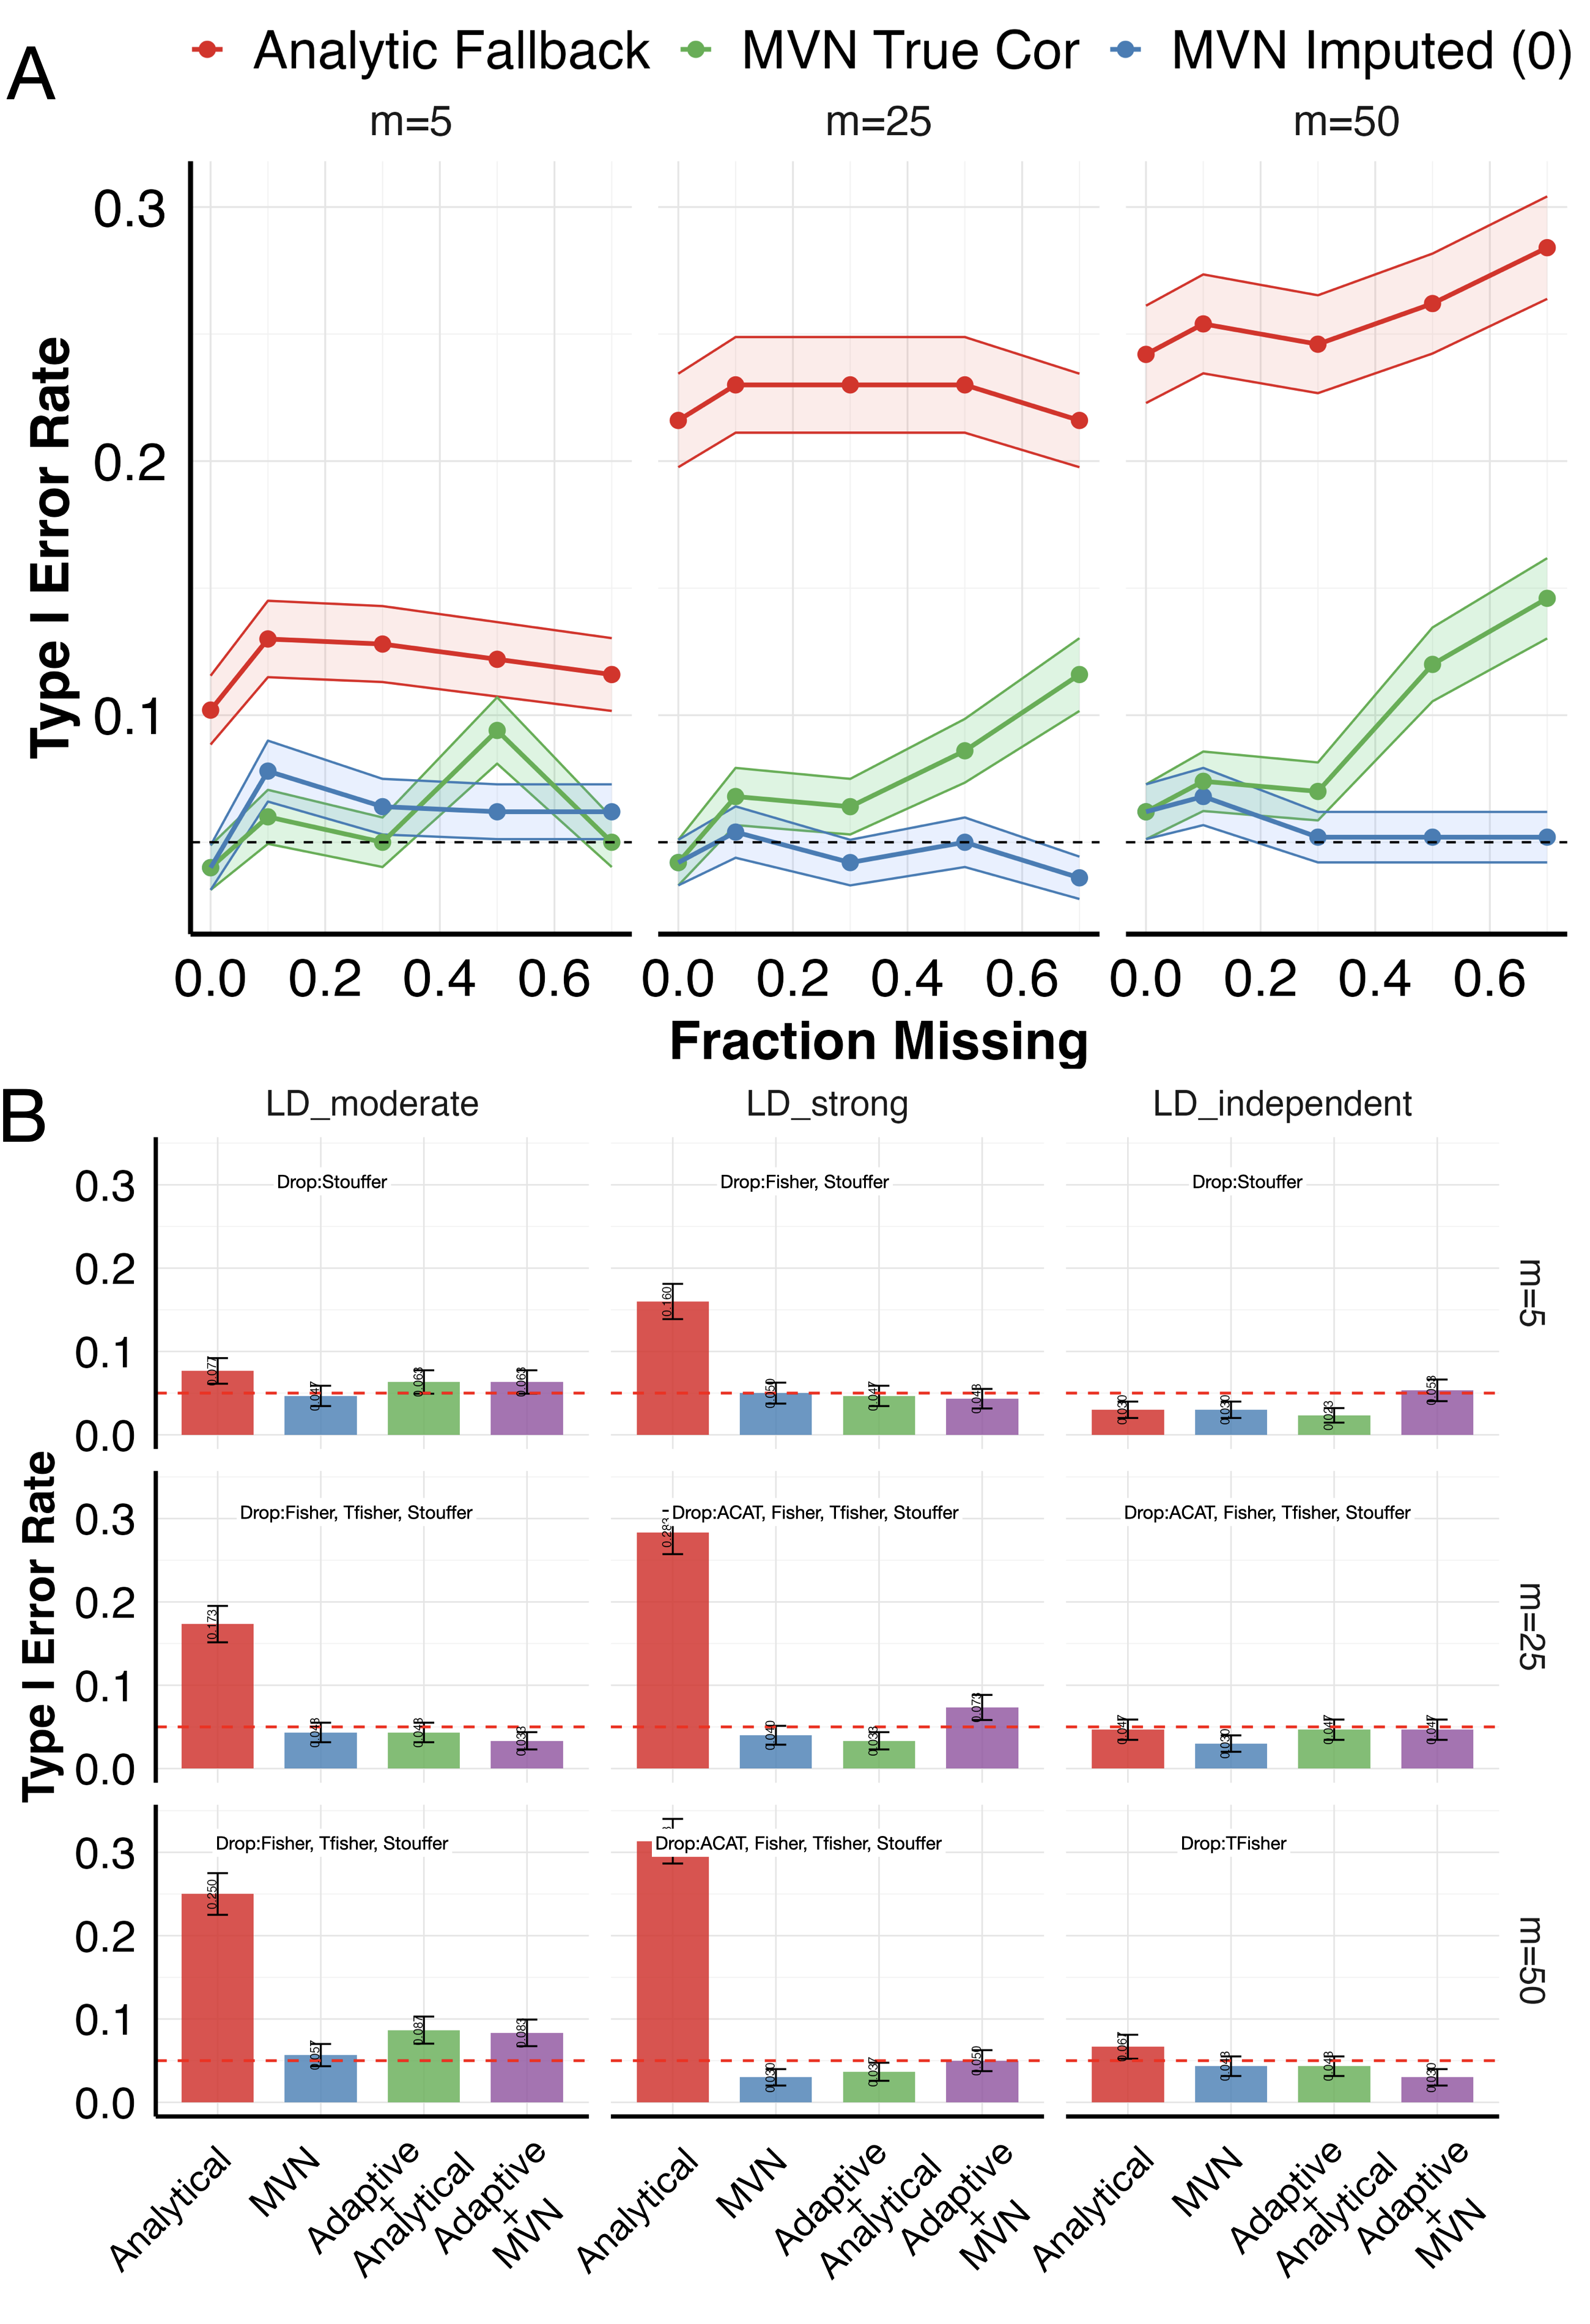
\includegraphics[width=\textwidth]{Figures/SuppFig/SuppFig3.Type_1_Error_vs_Missing_Correlation.png}
    \caption{\textbf{Type I error diagnostics under missing correlations and adaptive omnibus variants.}
    \textbf{A.} Using the same missing-correlation framework as Fig.~3A, we report empirical type I error of the omnibus test at $\alpha = 0.05$ (dashed line) across fractions missing and pathway sizes. The analytic fallback shows elevated false-positive rates in the presence of LD, while MVN-based approaches substantially improve error control. Consistent with Fig.~3A, the imputed-zero MVN strategy maintains type I error closer to nominal across missingness levels.
    \textbf{B.} For the four omnibus variants in Fig.~3B, we report empirical type I error at $\alpha = 0.05$ (dashed line). The LD-aware MVN omnibus maintains near-nominal error control across LD regimes and pathway sizes, whereas the analytical approach exhibits inflation under LD. The adaptive omnibus shows condition-dependent departures, often conservative and sometimes unstable under stronger LD, reinforcing that explicit MVN calibration is the most reliable approach for controlling false positives under LD.}
\end{figure*}

\subsection{From SNP associations to pathway-level aggregation}

We performed genome-wide association studies (GWAS) to characterize the genetic architecture of two traits in plants and animals. In \textit{Arabidopsis thaliana}, we examined BIO6, defined as the minimum temperature of the coldest month, using accessions from the 1001 Genomes Project to capture variation in long-term winter severity across the species' range. In \textit{Drosophila melanogaster}, we investigated starvation resistance as survival under food deprivation and conducted sex-stratified GWAS that replicated previously reported associations. In both datasets, the Manhattan plots revealed polygenic architectures, with multiple loci of modest effect contributing to distributed genome-wide association signals. Such patterns are consistent with complex traits in which many variants contribute small effects. Under this architecture, biological interpretation is often better achieved by shifting from individual loci to higher-order functional units such as pathway enrichments. We therefore performed LD-aware gene-level aggregation using MAGMA and summarized pathway-level evidence using CATFISH.

\begin{figure*}[!t]
    \centering
    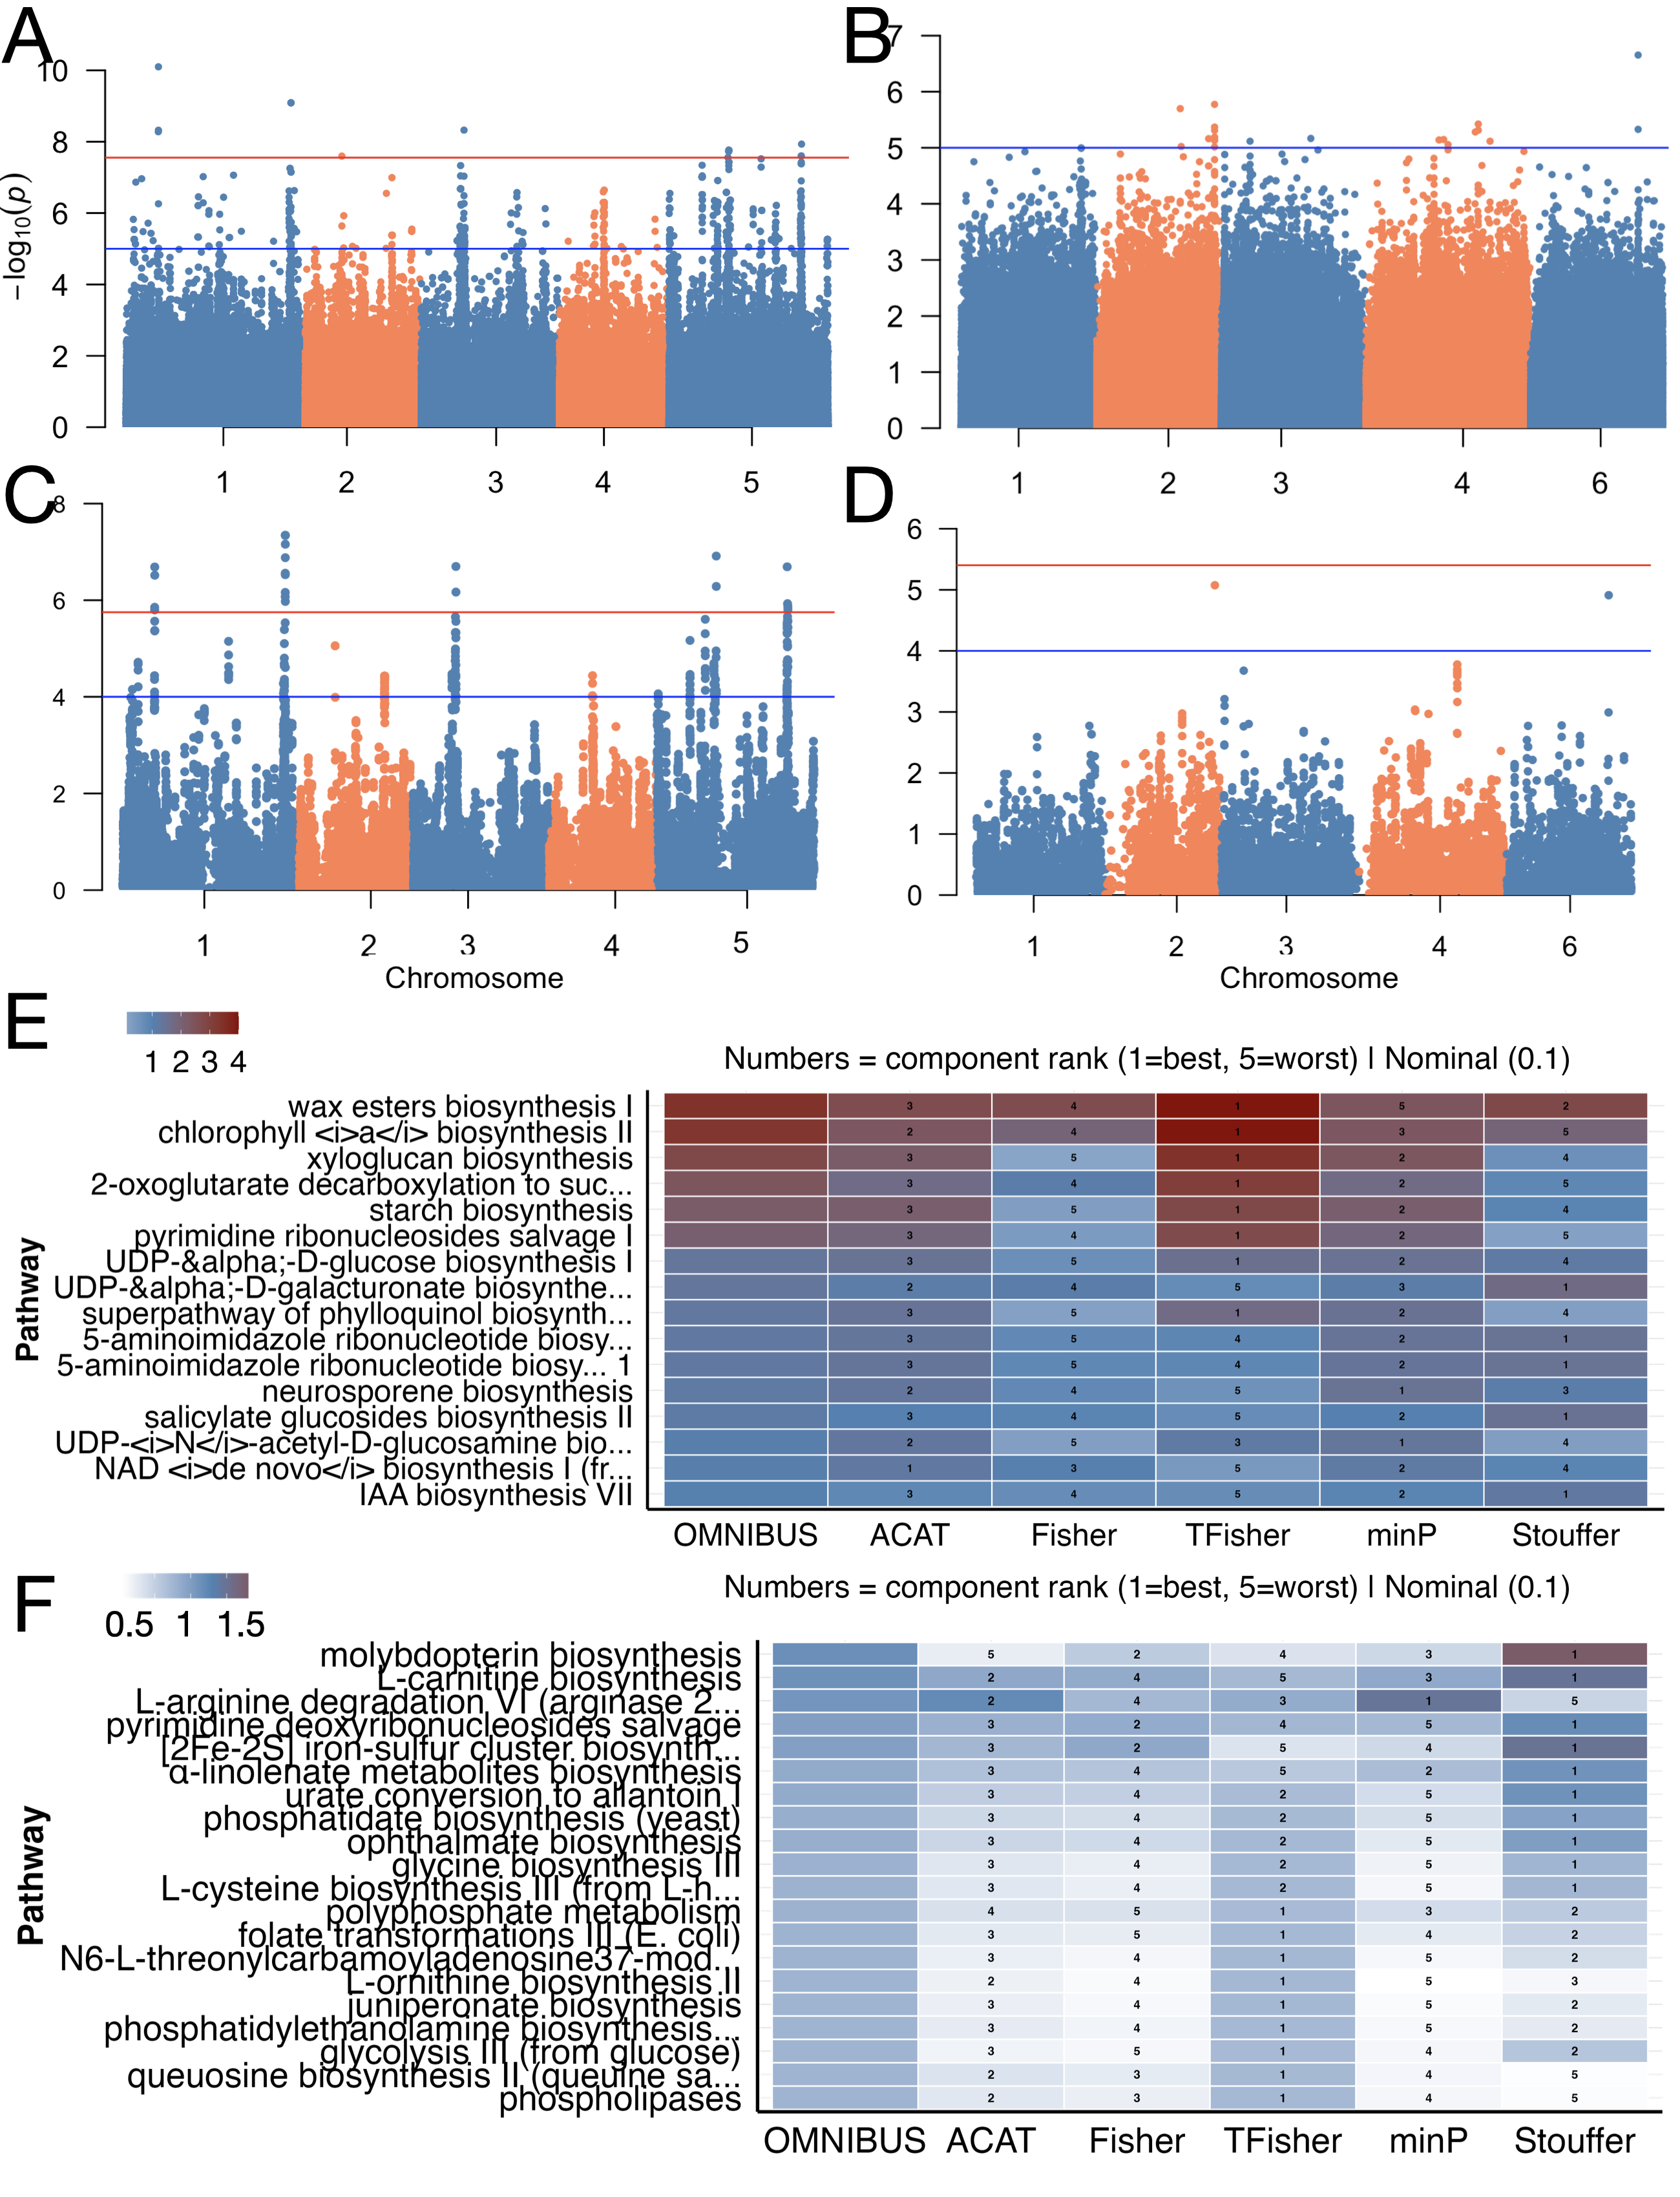
\includegraphics[width=\textwidth]{Figures/Fig4.Mahattan_arabidopsis_fly/Fig4.Manhattan.png}
    \caption{\textbf{From SNP-level association to gene- and pathway-level inference in Arabidopsis and Drosophila.}
    \textbf{A,B} GWAS Manhattan plots showing SNP-level association signals for \textit{Arabidopsis thaliana} BIO6 and \textit{Drosophila melanogaster} starvation resistance. Points show $-\log_{10}(P)$ for each variant, with alternating colors indicating chromosomes.
    \textbf{C,D} MAGMA gene-level association results for the corresponding GWAS, highlighting loci where aggregated SNP evidence yields stronger gene-level support.
    \textbf{E,F} CATFISH pathway enrichment summaries for the top pathways in \textit{Arabidopsis} BIO6 and \textit{Drosophila} starvation resistance. Heatmaps show calibrated $-\log_{10}(P)$ for the CATFISH omnibus and each component test (ACAT, Fisher, TFisher, minP, Stouffer), with rows ordered by omnibus significance. The final column indicates the leading component test for each pathway.}
\end{figure*}

To translate SNP-level associations into gene-level evidence while accounting for LD, we applied MAGMA to the GWAS datasets. MAGMA aggregates SNP-level association statistics within predefined gene boundaries using a multiple regression framework that incorporates LD structure among variants, thereby generating gene-level $p$-values that represent the cumulative genetic signal attributable to each gene. In \textit{Arabidopsis}, MAGMA analysis maintained the overall signal while reducing noise from isolated SNPs, leading to significant gene-level associations across all chromosomes. In \textit{Drosophila}, MAGMA similarly produced a set of gene-level associations indicative of a broadly distributed genetic architecture. These outputs served as the shared gene-level input for downstream CATFISH pathway enrichment analyses.

We next applied CATFISH to translate MAGMA gene-level association statistics into pathway-level inference using five complementary component tests: ACAT, Fisher's method, TFisher, the minimum-$p$ test (minP), and Stouffer's $Z$-score method. In the \textit{Arabidopsis} BIO6 analysis, CATFISH highlighted pathways enriched for cold-associated genetic signal, including processes linked to wax ester biosynthesis and starch metabolism. In \textit{Drosophila}, CATFISH similarly revealed enrichment of pathways related to amino acid and lipid metabolism, with Stouffer often providing the strongest support among the component tests and TFisher sometimes leading. Pathways were ranked by the omnibus $p$-value, and the final column reports the leading component test, that is, the statistic yielding the smallest calibrated component $p$-value for that pathway. In both datasets, the smallest calibrated component $p$-value varied across pathways, reflecting the dominant signal architecture rather than any systematic bias. For example, TFisher often yielded the lowest $p$ in \textit{Arabidopsis}, whereas Stouffer often did in the fly (Fig.~4E,F). Importantly, multiple pathways showed different best tests, including ACAT, minP, and Fisher, illustrating that CATFISH adapts to pathway-specific signal structure rather than recapitulating a single statistic.

\subsection{Component gene-set tests capture distinct pathway signals across traits and species}

To evaluate whether CATFISH's component pathway tests provide non-redundant information, rather than repeatedly detecting the same pathways, we compared the five component statistics (ACAT, Fisher, TFisher, minP, and Stouffer) using \textit{Arabidopsis} BIO6 and \textit{Drosophila} starvation resistance as contrasting case studies. While multiple tests are expected to exhibit overlapping sensitivity to related signal patterns, each method implicitly specifies a distinct enrichment model and may consequently prioritize different classes of pathways.

\begin{figure*}[!t]
    \centering
    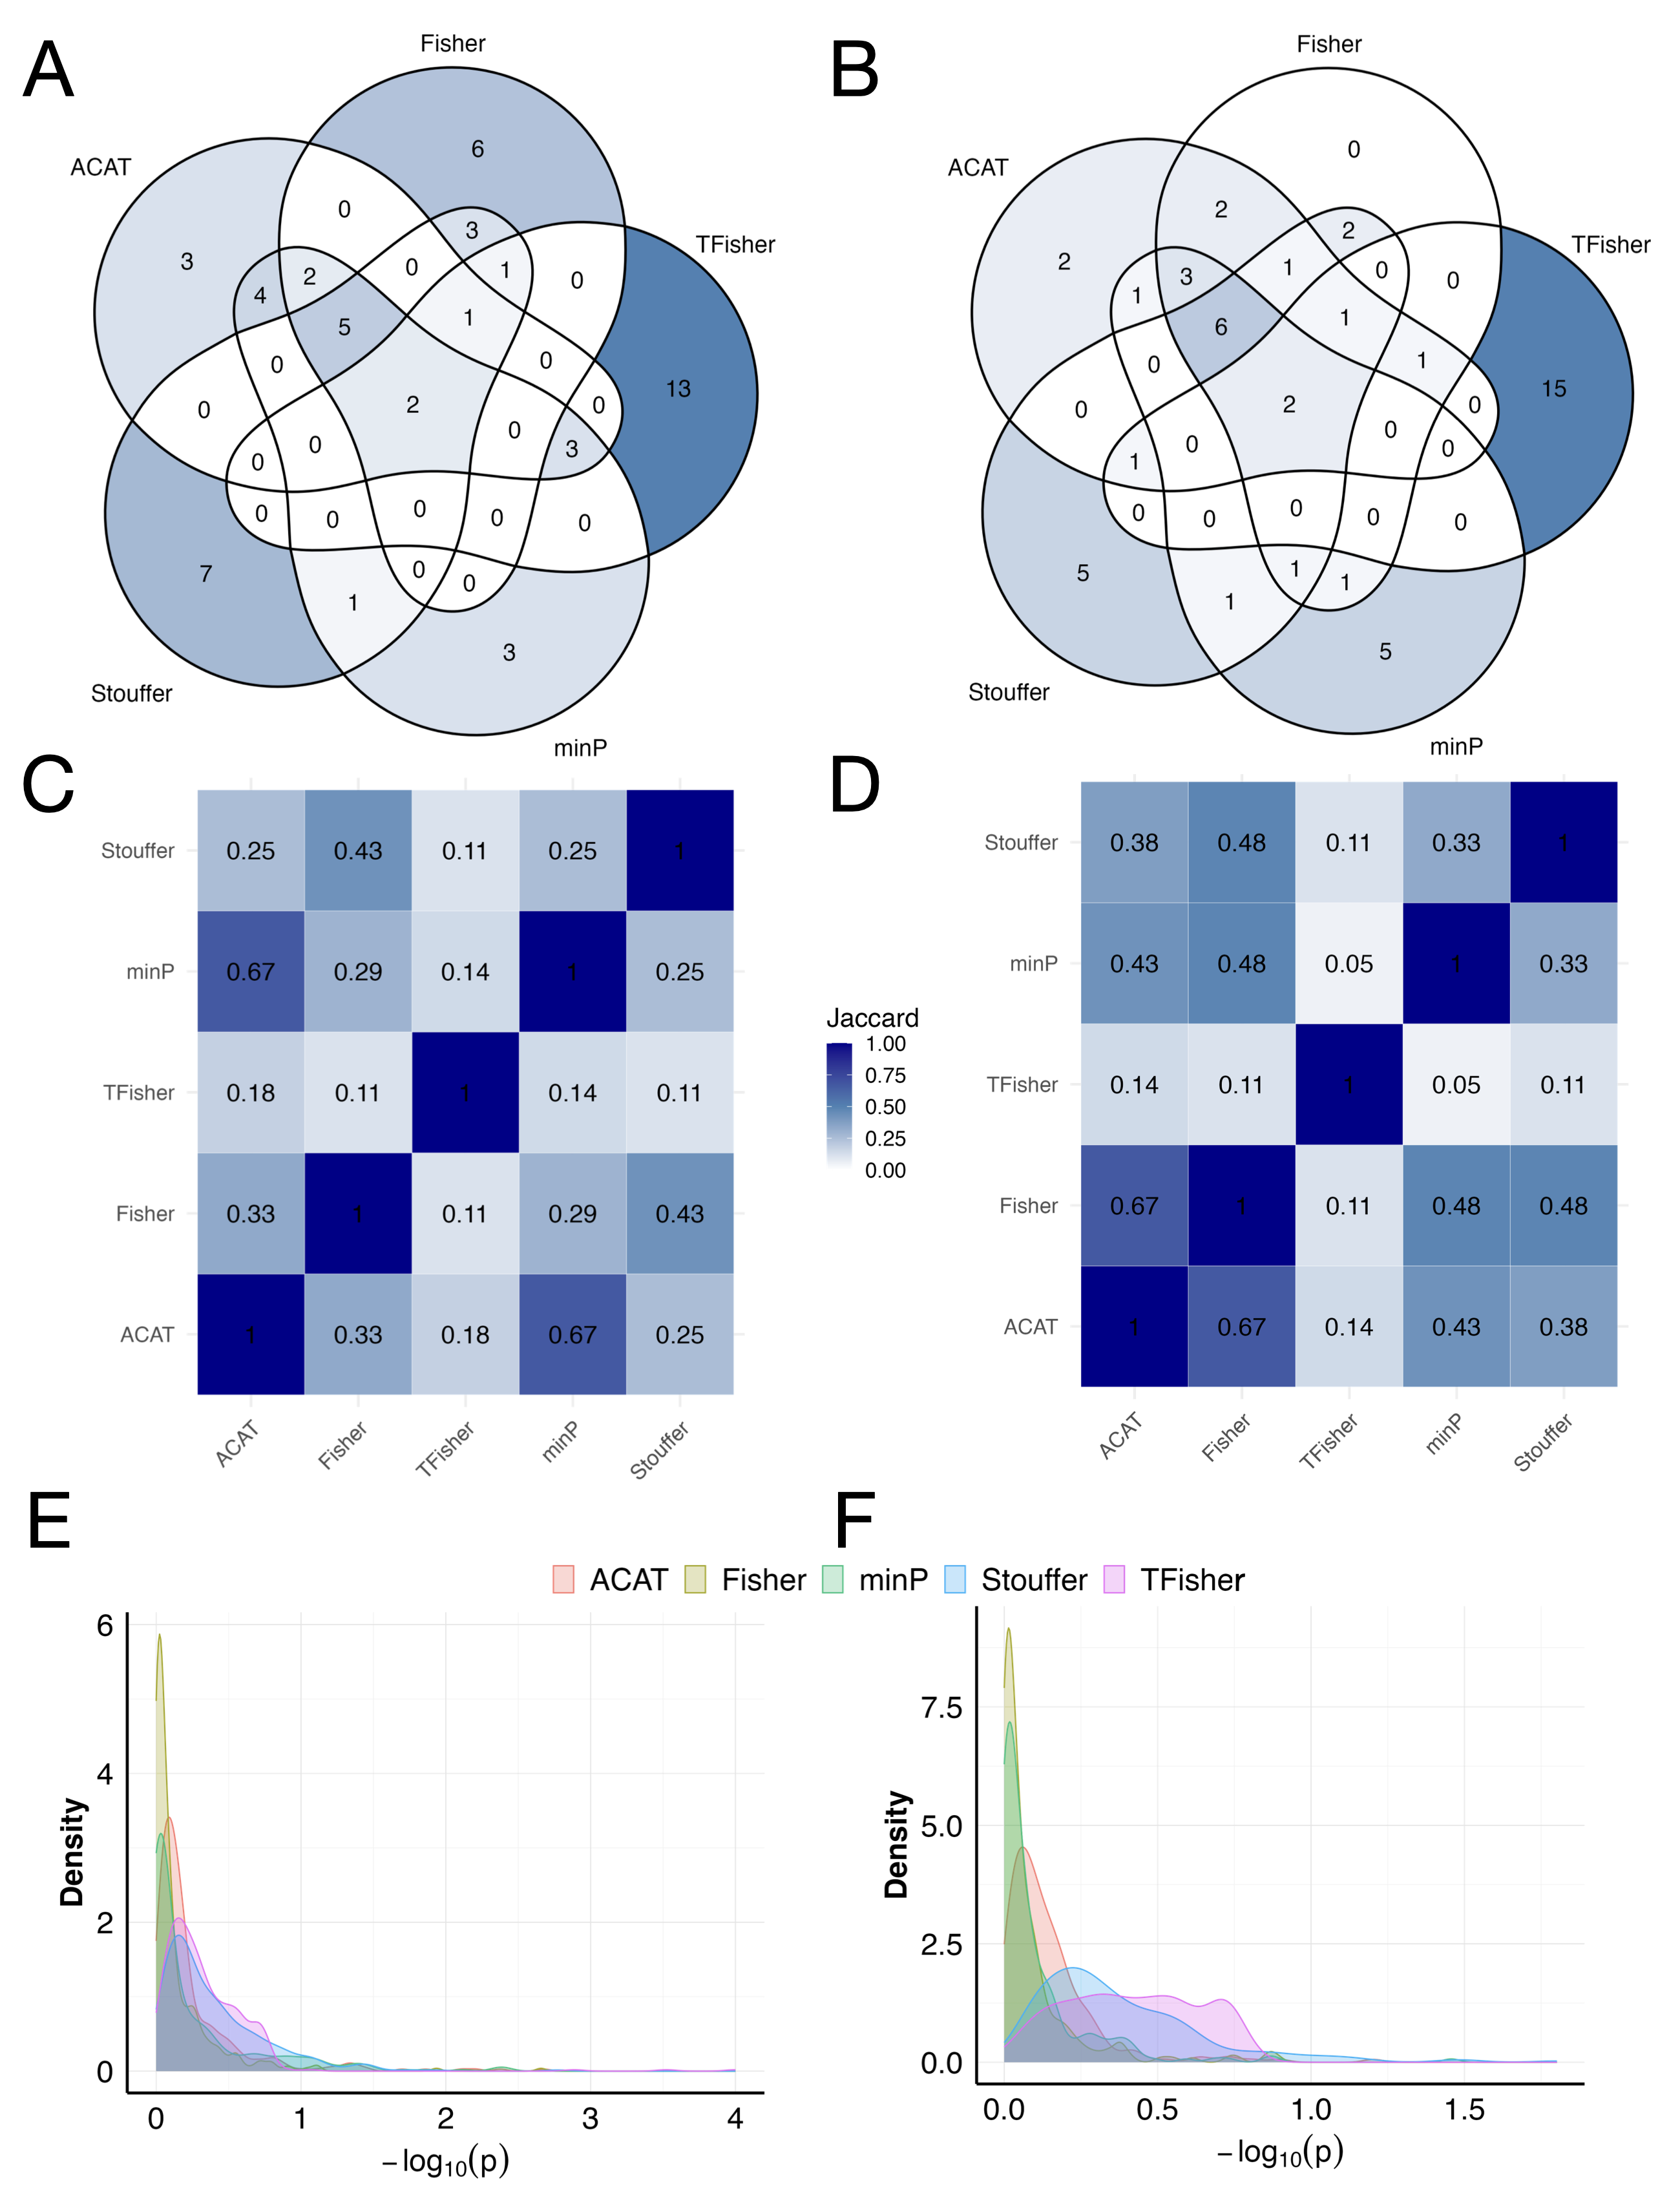
\includegraphics[width=\textwidth]{Figures/Fig5.component_test_arabidopsis_fly/Fig5.Compare_component_test_arabidopsis.png}
    \caption{\textbf{Component pathway tests capture unique pathway classes despite shared gene-level inputs.}
    \textbf{A,B} Overlap among significant pathways detected by ACAT, Fisher, adaptive TFisher, minP, and Stouffer in \textit{Arabidopsis} and \textit{Drosophila}. TFisher yields the largest number of hits, consistent with adaptive tail selection over a $\tau$-grid.
    \textbf{C,D} Pairwise Jaccard similarity of discovered pathway sets. ACAT and minP cluster strongly in both datasets; in fly, Fisher shows increased similarity to ACAT/minP, and Fisher--Stouffer similarity indicates agreement under coordinated multi-gene enrichment.
    \textbf{E,F} Distributions of pathway-level $-\log_{10}(p)$. Fisher shows the strongest mass near null-like values, whereas Stouffer and TFisher show heavier right tails. All component $p$-values are calibrated under the same dependence-preserving MVN null generator.}
\end{figure*}

Across both datasets, the overlap analyses revealed a substantial number of discoveries that were specific to individual methods. A considerable proportion of statistically significant pathways were unique to particular component tests, rather than being shared across all approaches. In particular, TFisher contributed the largest set of method-specific pathways in both the \textit{Arabidopsis} and \textit{Drosophila} datasets. This observation is consistent with the adaptive soft-thresholding principle underlying TFisher: by assessing pathway enrichment over a grid of truncation thresholds ($\tau$ values) and selecting the most informative configuration, TFisher is able to detect pathway-level signals that are moderately dense or concentrated within specific gene subsets without relying on a single fixed cutoff. Overall, TFisher effectively interpolates between sparse and diffuse signal regimes, broadening the range of pathways it can identify relative to single-parameter procedures.

Despite these method-specific distinctions, the component tests were not statistically independent, and their pairwise overlap exhibited a systematic and interpretable structure. Jaccard similarity matrices (Fig.~5C,D) demonstrated that ACAT showed the highest similarity to minP, particularly in \textit{Drosophila}, consistent with both procedures being highly responsive to sparse-driver architectures. By contrast, Fisher's and Stouffer's methods exhibited greater similarity to each other than to any other method, reflecting their shared propensity to aggregate weak-to-moderate evidence across many genes. These qualitative relationships were also reproduced by correlation-based measures (Supp.~Fig.~4C,D). Overall, these results indicate that the observed similarity structure is robust to the choice of overlap metric: the methods form partially overlapping sets, but no method is redundant with or collapses onto another.

Differences in behavior were also evident in the global $p$-value distributions. Fisher's method was concentrated closer to null-like values, whereas TFisher and Stouffer exhibited heavier right tails in $-\log_{10}(p)$, consistent with these procedures identifying a greater number of strongly enriched pathways in scenarios characterized by many modest gene-level effects.

\begin{figure*}[!t]
    \centering
    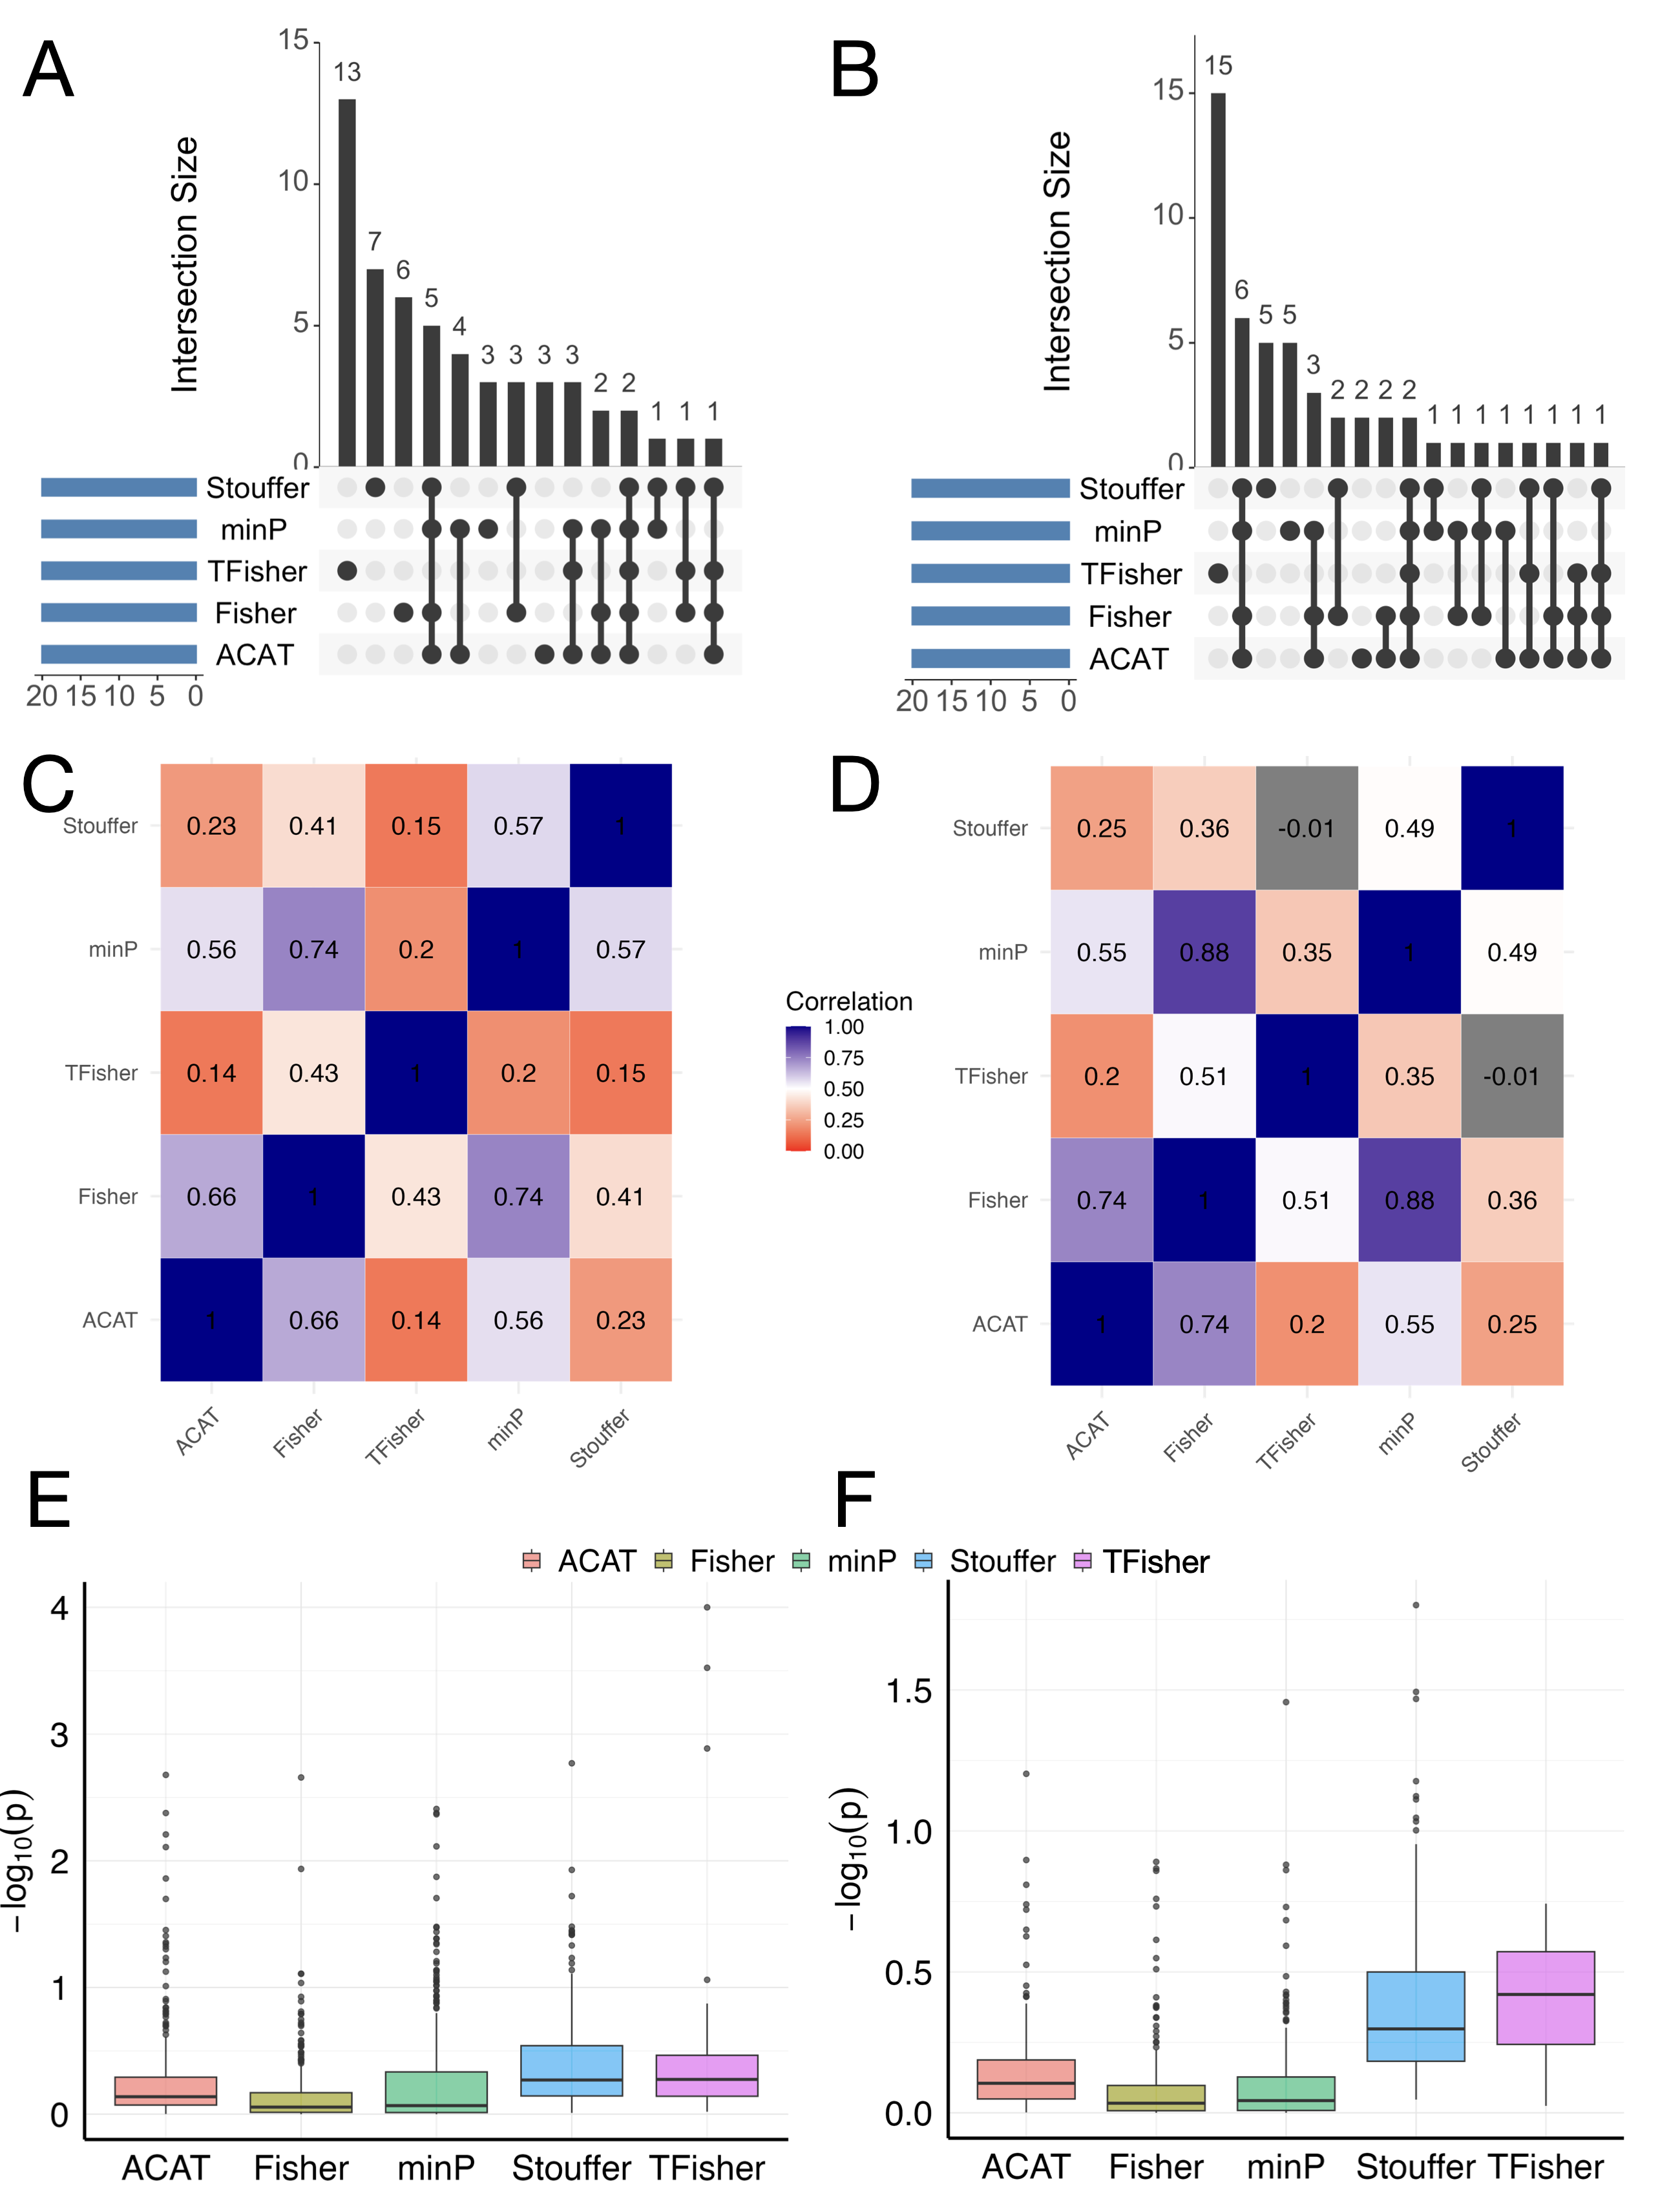
\includegraphics[width=\textwidth]{Figures/SuppFig/SuppFig4.Compare_component_test_arabidopsis.png}
    \caption{\textbf{Extended comparison of component pathway tests.}
    \textbf{A,B} UpSet plots summarize the intersection structure among significant pathway sets, confirming that each test contributes unique discoveries in both \textit{Arabidopsis} and fly.
    \textbf{C,D} Pairwise association patterns recapitulate the main figure.
    \textbf{E,F} $p$-value distributions show heavier tails for Stouffer and TFisher; calibration under the dependence-preserving null is therefore required to ensure these are not false-positive artifacts.}
\end{figure*}

These analyses show that although component tests exhibit structured correlation, most notably ACAT with minP and Fisher with Stouffer, they nonetheless recover partially distinct sets of pathways, with TFisher contributing substantial additional discoveries in both \textit{Arabidopsis} and \textit{Drosophila}. This pattern supports the design of CATFISH, namely combining complementary statistics to improve coverage across heterogeneous pathway-level signal architectures that differ across traits, species, and overall GWAS signal scale.

\subsection{The omnibus aggregates component tests rather than recapitulating a single test}

\begin{figure*}[!t]
    \centering
    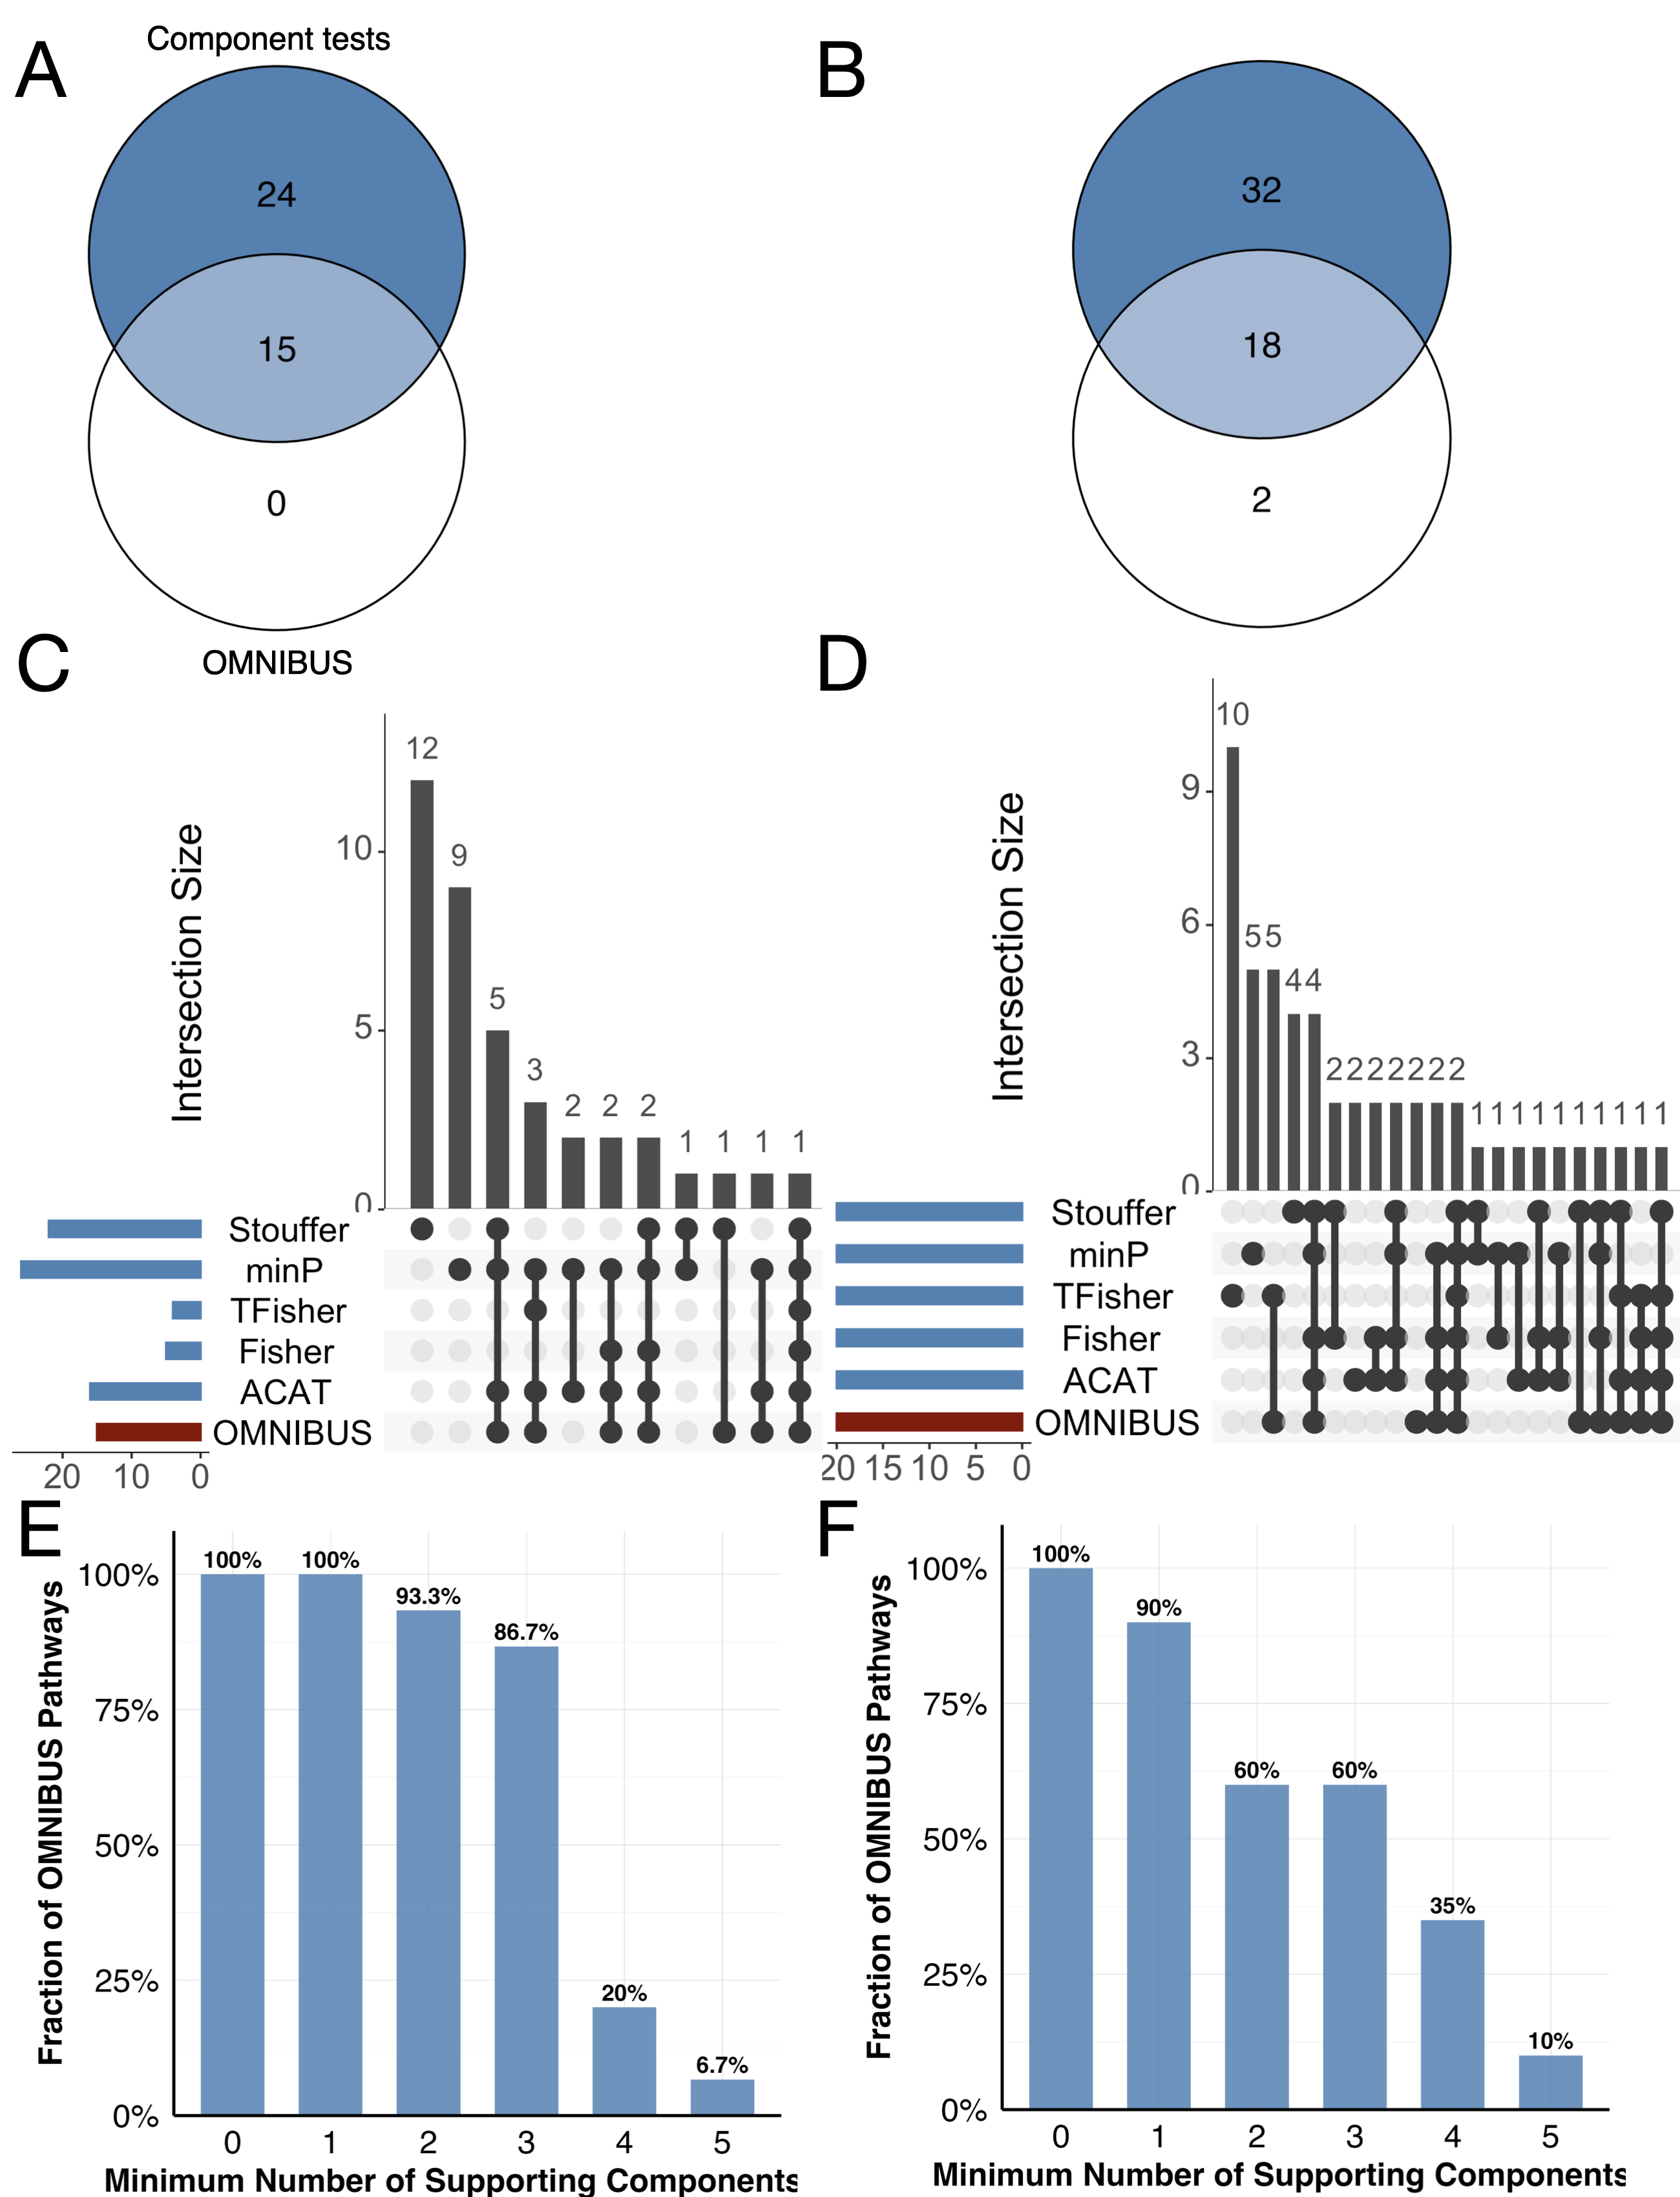
\includegraphics[width=\textwidth]{Figures/Fig6.omni_vs_component_arabidopsis/Fig6.omni_vs_component_arabidopsis.png}
    \caption{\textbf{Omnibus behaves as a broad union, not a narrow intersection.}
    \textbf{A,B} Panels compare the omnibus significant set to the union of component significant sets for \textit{Arabidopsis} and fly, demonstrating union-consistency in \textit{Arabidopsis} and a small number of omnibus-only calls in fly consistent with aggregation of sub-threshold component evidence.
    \textbf{C,D} UpSet-style summaries show that omnibus discoveries concentrate in multi-method overlaps while still permitting a limited number of architecture-specific calls.
    \textbf{E,F} The fraction of omnibus pathways supported by at least $k$ component tests indicates stronger multi-test support in \textit{Arabidopsis} and greater heterogeneity in fly.}
\end{figure*}

We next investigated whether the MVN-calibrated omnibus operates as a true integrator or collapses to an effective surrogate for a single component test. In \textit{Arabidopsis}, the discovery set identified by the omnibus procedure was fully contained within the union of discoveries from the individual component tests under the same significance threshold. This demonstrates that the omnibus is not producing unique signals that are decoupled from its constituent evidence layers. In \textit{Drosophila}, however, the omnibus recovered the majority of pathways supported by at least one component test but additionally identified a small subset of pathways not detected by any single component. This behavior illustrates a key strength of the omnibus framework: it can yield statistical significance when multiple component $p$-values are individually suggestive but do not cross the specified threshold on their own. Such omnibus-only hits should not automatically be interpreted as artifacts; rather, they may reflect genuine synergy across component tests and must be evaluated under rigorous null calibration.

The higher-order intersection patterns showed that omnibus-significant pathways were not predominantly driven by calls unique to a single method; instead, they were enriched for multi-test overlap. In \textit{Arabidopsis}, a substantial proportion of omnibus-significant pathways remained significant even under increasingly stringent multi-test support criteria, for example requiring support from at least two or three component methods. By contrast, in \textit{Drosophila}, multi-test support was generally weaker, with a larger fraction of pathways supported by only one or a small number of component methods. This suggests that the \textit{Arabidopsis} BIO6 signal is more consistently detectable across multiple signal archetypes, whereas the \textit{Drosophila} dataset contains a higher proportion of architecture-specific signals detectable only by certain classes of enrichment tests.

\begin{figure*}[!t]
    \centering
    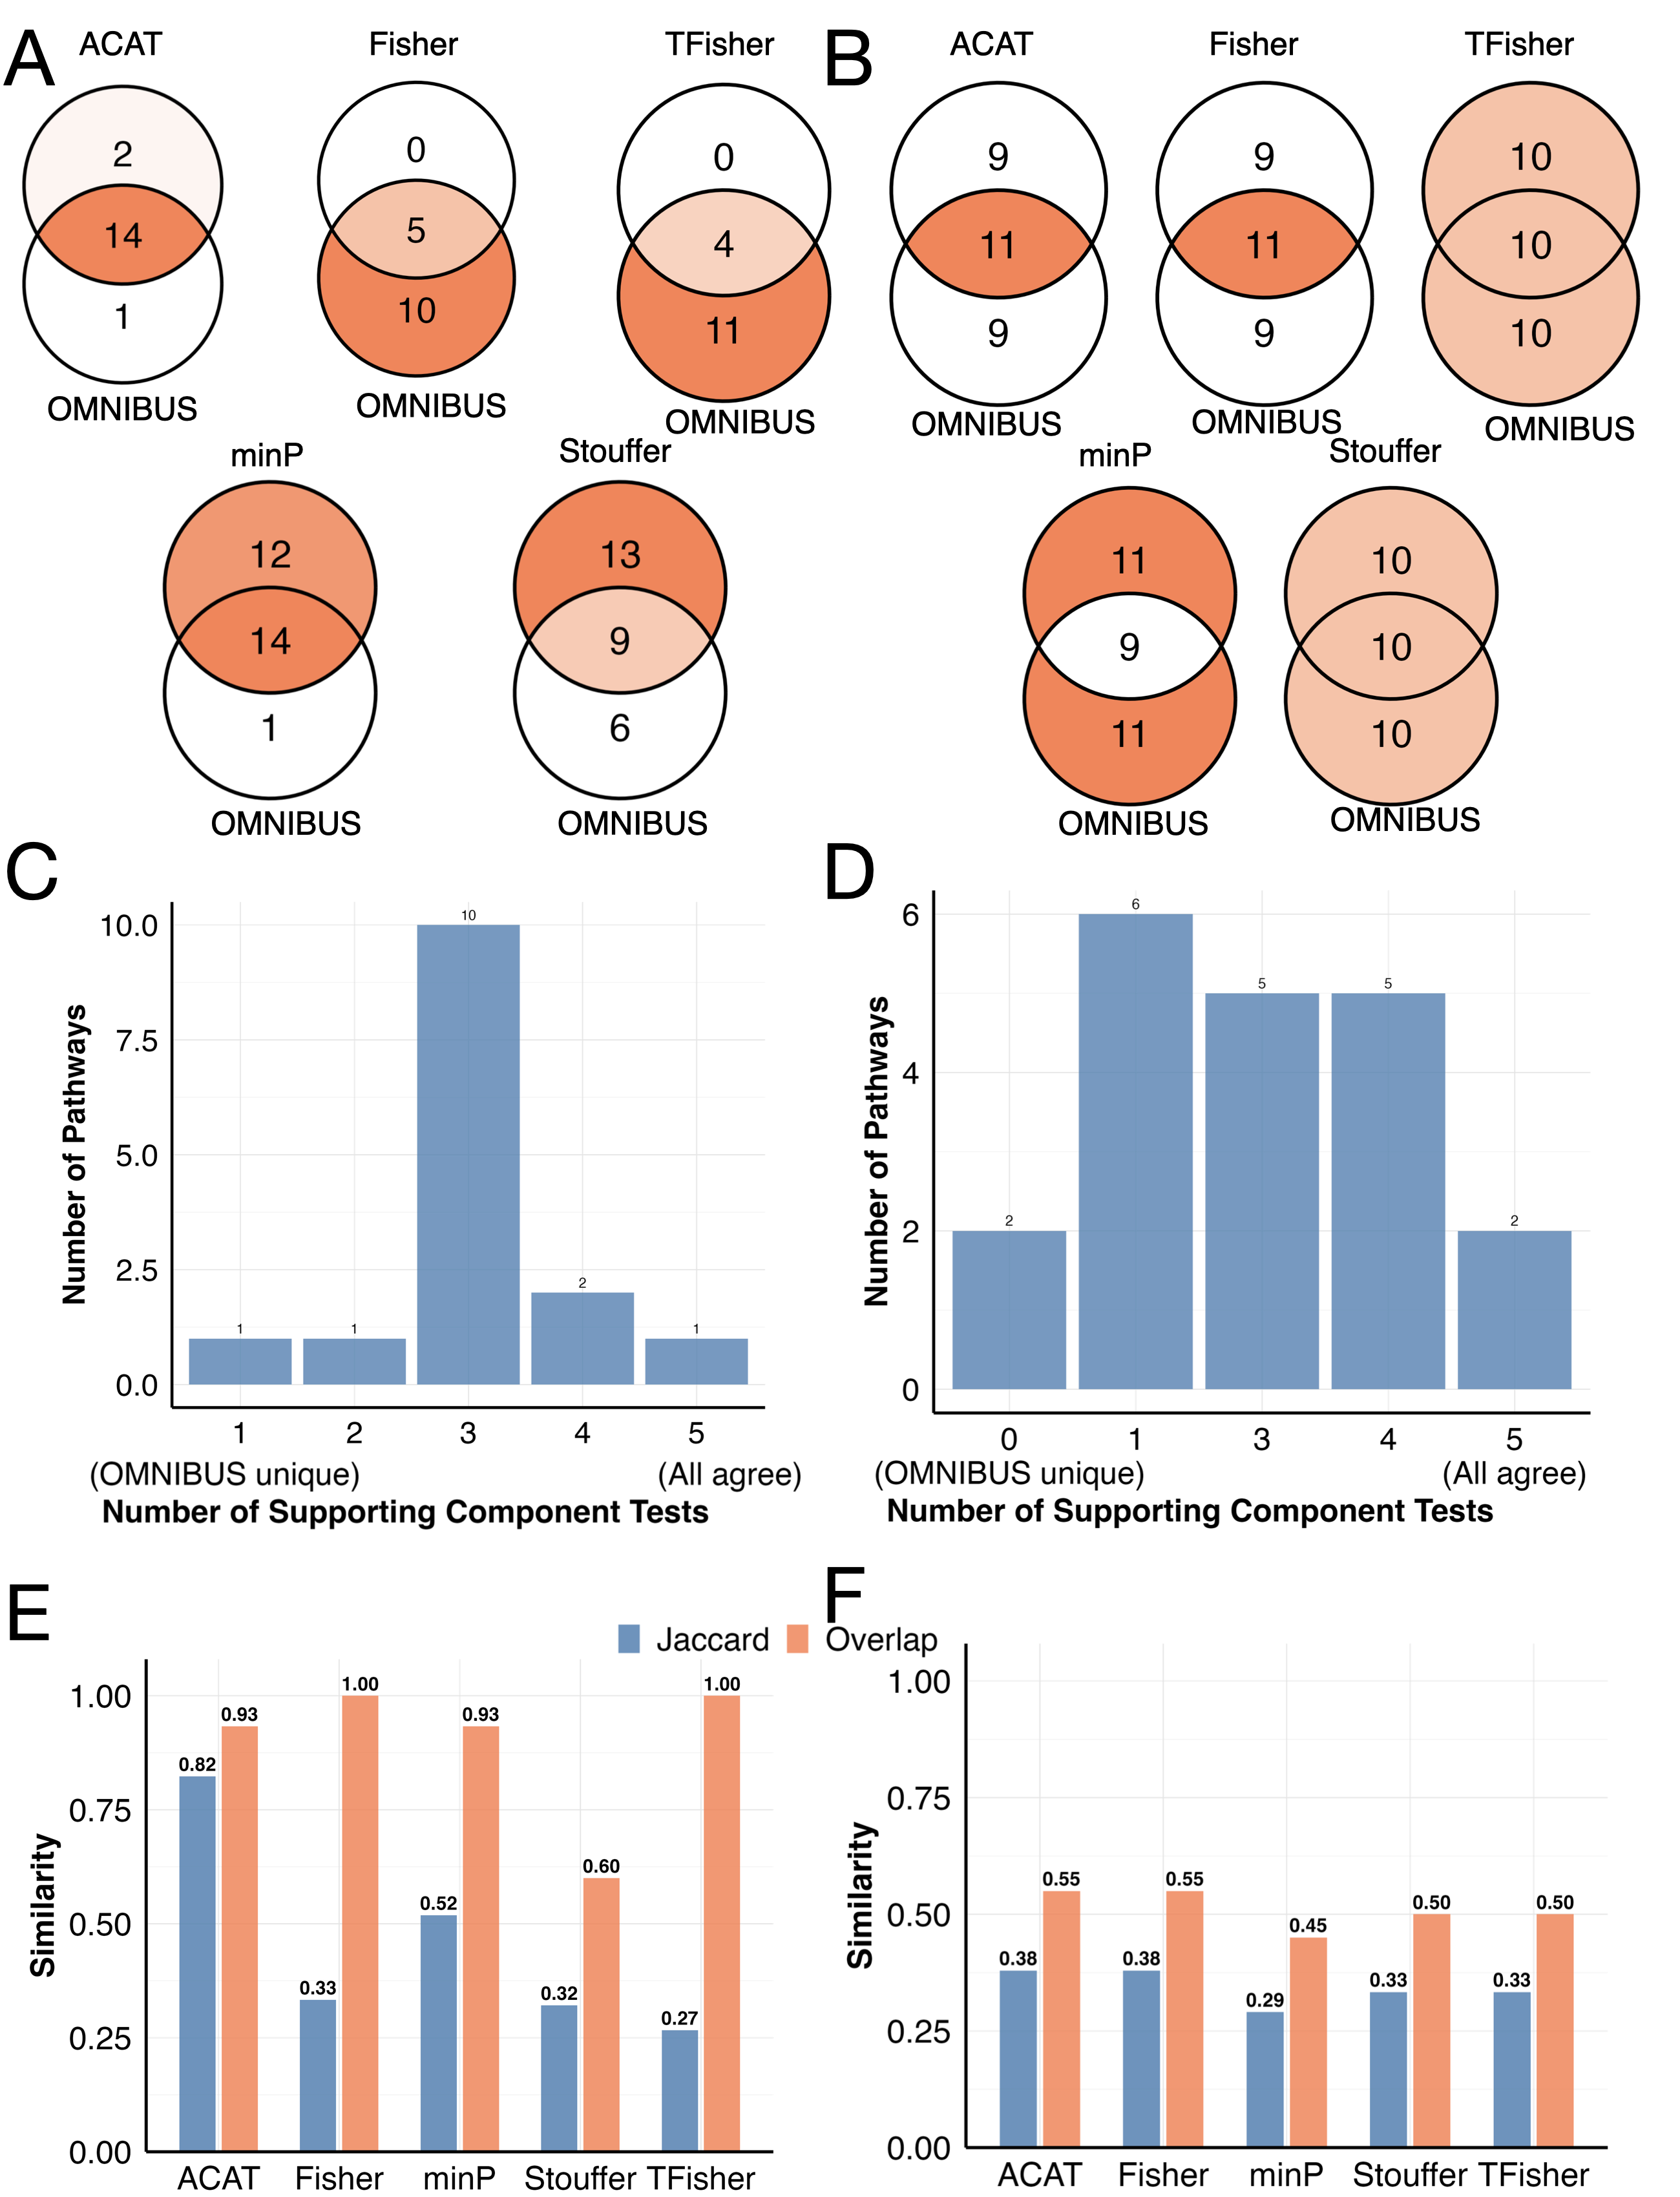
\includegraphics[width=\textwidth]{Figures/SuppFig/SuppFig5.omni_vs_component_arabidopsis.png}
    \caption{\textbf{Component-by-component decomposition of omnibus overlap.}
    \textbf{A,B} Pairwise overlaps between the omnibus and each component test in \textit{Arabidopsis} and fly.
    \textbf{C,D} Distribution of omnibus-significant pathways across the number of supporting component tests, reinforcing that omnibus calls are enriched for multi-test support but are not identical to any single component.}
\end{figure*}

The similarity metrics clarify an important subtlety: the overlap proportion and the Jaccard index answer different questions. The overlap proportion is asymmetric, reflecting how much of a component's discovery set is recovered by the omnibus, whereas the Jaccard index is symmetric and penalizes methods that call many extra pathways beyond the shared set. Consequently, in \textit{Arabidopsis}, cases of high overlap but only moderate Jaccard indicate that a component's calls are largely contained within the omnibus, while the total union remains large because one set contains many additional pathways. In the fly dataset, overlap and Jaccard were more similar in magnitude, implying that component and omnibus discovery set sizes were closer and that the union was less dominated by one method's extra calls. Collectively, Fig.~6 and Supp.~Fig.~5 support the conclusion that the omnibus is broad in the signal types it can detect, yet selective in what it ultimately reports, behaving as an evidence integrator rather than a permissive union rule or a disguised single-component test.

\subsection{MVN global-null diagnostics support overall calibration}

To verify that differences in discovery patterns reflect power differences rather than miscalibration, we assessed all component tests and the omnibus procedure under a dependence-preserving global null using MVN resampling (Supp.~Fig.~6). The Q--Q plots compare the empirical $p$-value distributions to the theoretical uniform distribution implied by the null hypothesis, and the genomic control factor $\lambda$ provides a scalar summary of global inflation or deflation, with $\lambda \approx 1$ indicating appropriate calibration. Operationally, $\lambda$ captures whether the bulk of null test statistics is globally over- or under-dispersed relative to expectation, whereas empirical type I error directly evaluates threshold-level calibration via the observed rejection rate $\Pr(p < \alpha)$ at a chosen $\alpha$. In both datasets, ACAT, Fisher's method, minP, and Stouffer's method yielded $\lambda$ values close to 1, consistent with well-controlled null behavior under the MVN-based calibration scheme. The omnibus test was likewise close to null in both datasets, slightly conservative in \textit{Arabidopsis} and near 1 in \textit{Drosophila}, a desirable property for a combined procedure intended to maintain stable type I error control across heterogeneous pathway architectures.

The main calibration exception was TFisher in the female fly null diagnostics, which showed a markedly elevated $\lambda$, indicating a strong departure from the expected null. The empirical type I error at $\alpha = 0.05$ remained at or below nominal, indicating that TFisher's deviation was not simply more false positives at 0.05. Instead, the result is more consistent with a null distribution shape or scale mismatch that affects the broader $p$-value spectrum without necessarily manifesting as excess rejections at a single threshold. Importantly, the omnibus did not inherit this instability, as both its $\lambda$ and type I error remained close to nominal, consistent with the omnibus functioning as a stabilizing integrator that limits dependence on the idiosyncratic behavior of any single component test. These diagnostics support the conclusion that the CATFISH MVN framework is approximately nominally calibrated for most individual component tests and for the omnibus statistic, even though a subset of components may still exhibit residual miscalibration.

\begin{figure*}[!t]
    \centering
    \includegraphics[width=\textwidth]{Figures/SuppFig/SuppFig6.null_calibration_combined.png}
    \caption{\textbf{MVN null diagnostics support calibrated inference.}
    \textbf{A} Q--Q plots compare observed versus expected $p$-values under dependence-preserving MVN resampling for each component and the omnibus in \textit{Arabidopsis} and fly.
    \textbf{B} Genomic control ($\lambda$) summarizes calibration, showing elevated $\lambda$ for TFisher in fly while the omnibus remains near 1.
    \textbf{C} Type I error at $\alpha = 0.05$ confirms near-nominal rejection rates overall, supporting interpretation of component differences as sensitivity to distinct signal architectures rather than systematic false positives.}
\end{figure*}

\subsection{Candidate-gene prioritization integrates GWAS, MAGMA, and pathway evidence}

In Fig.~7A,B, we quantified the number of genes supported at each layer under the specified thresholds. For the \textit{Drosophila} analysis, the GWAS evidence layer was deliberately defined using a more permissive significance threshold, reflecting the observation that very few genes satisfy a Bonferroni cutoff. The median number of genes per pathway was lower in \textit{Drosophila} than in \textit{Arabidopsis}; consequently, pathway membership alone constituted a weaker filtering criterion in the fly analysis.

In \textit{Arabidopsis} (Fig.~7C), a visible subset of genes showed concordant evidence across layers, including support from all three layers, consistent with a mixture of strong locus-driven genes. In fly females (Fig.~7D), many top-ranked genes were supported by GWAS and MAGMA but lacked pathway/top-pathway support at the chosen pathway threshold, consistent with either a smaller or shallower pathway mapping, or with pathway-level signals being distributed across many modest genes rather than concentrating on the same top loci that drive GWAS and MAGMA.

Furthermore, genes in the top pathways were enriched for stronger MAGMA signals (Fig.~7E,F), with a clear shift in \textit{Arabidopsis} but a weaker or non-significant shift in fly, indicating that the pathway layer preferentially captures elevated gene-level association in \textit{Arabidopsis}, whereas in fly the enrichment signal is more diffuse.

\begin{figure*}[!t]
    \centering
    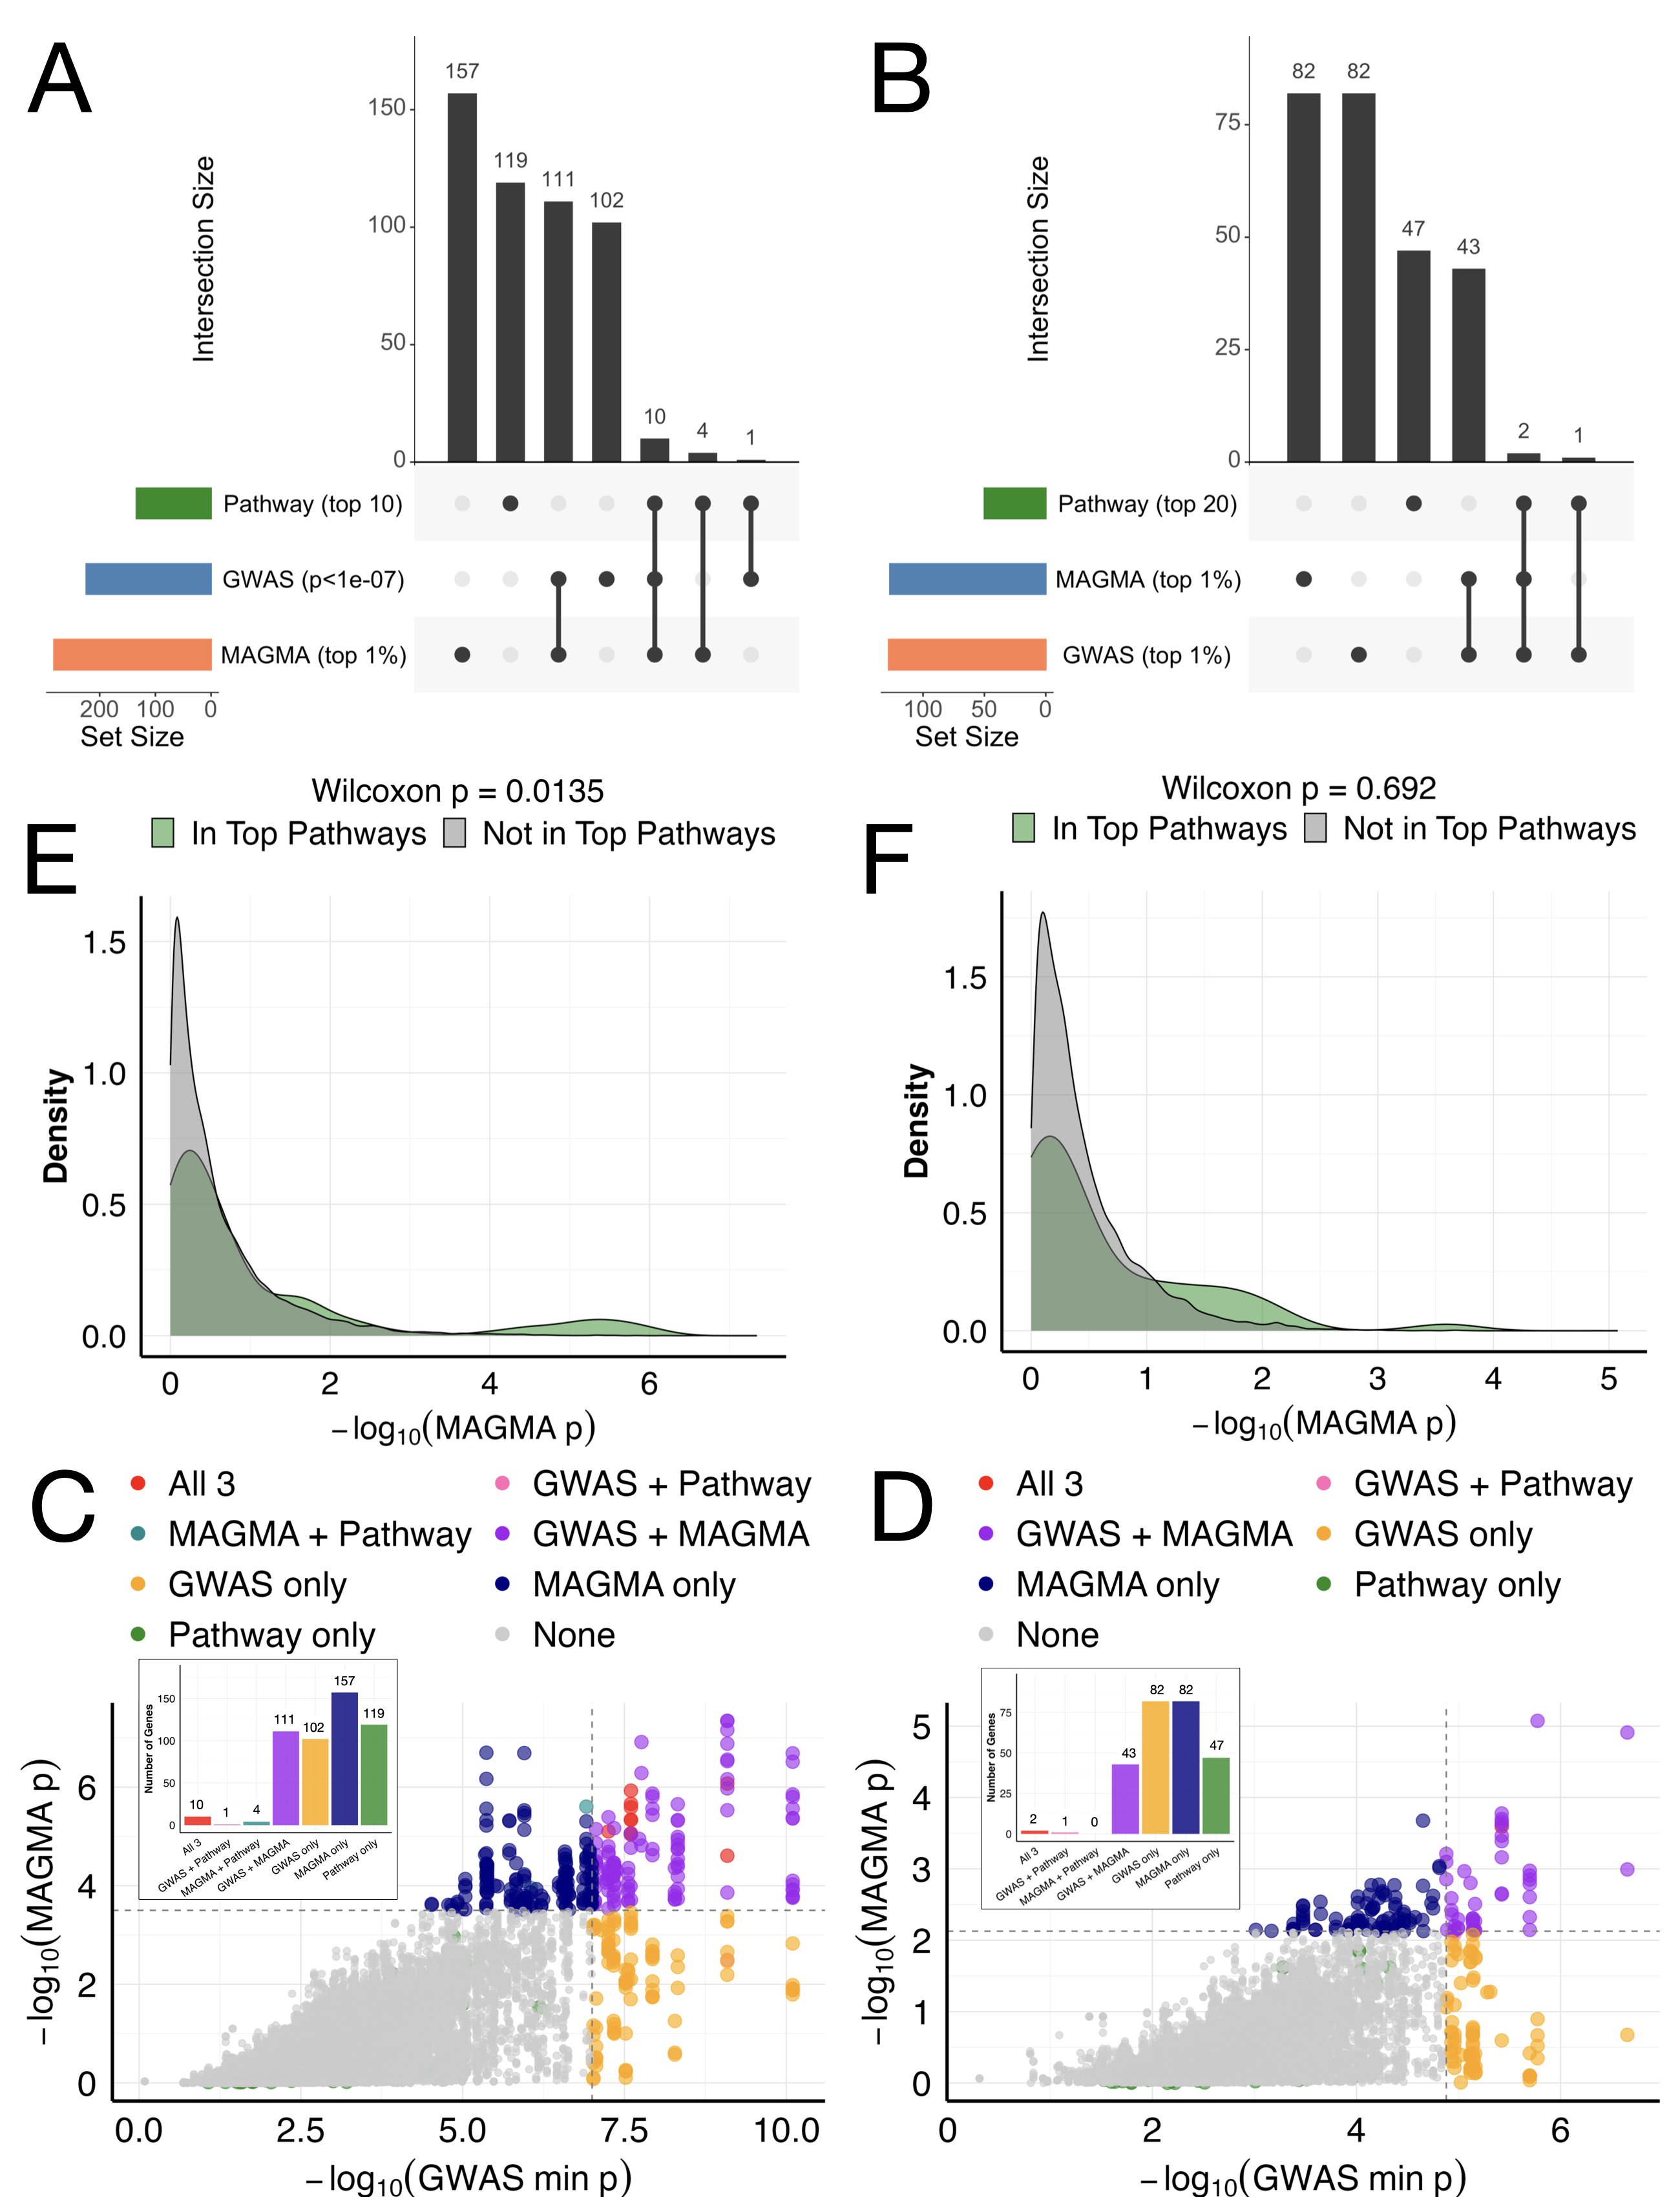
\includegraphics[width=\textwidth]{Figures/Fig7.candidate_gene_analysis_arabidopsis/Fig7.candidate_gene_analysis_arabidopsis.png}
    \caption{\textbf{Multi-layer candidate-gene prioritization integrates GWAS locus evidence, MAGMA gene-level association, and pathway enrichment.}
    Panels \textbf{A/C/E} show \textit{Arabidopsis} (BIO6) and panels \textbf{B/D/F} show female \textit{Drosophila} starvation resistance.
    \textbf{A,B} UpSet plots summarize overlap among genes supported by each layer at the thresholds used in the main analysis.
    \textbf{C,D} Gene-level concordance between GWAS and MAGMA: each point is a gene, with the x-axis showing GWAS locus evidence mapped to the gene ($-\log_{10}$ of the minimum GWAS $p$-value among mapped variants) and the y-axis showing MAGMA evidence ($-\log_{10}$ MAGMA $p$-value). Points are colored by which evidence layers support the gene.
    \textbf{E,F} Distribution of MAGMA evidence for genes inside versus outside top enriched pathways; green curves denote genes in top pathways and gray curves denote genes not in top pathways, with Wilcoxon $p$-values testing for a shift toward stronger MAGMA association among pathway genes.}
\end{figure*}

For each gene, \texttt{best\_pathway\_p} denotes the smallest calibrated pathway $p$-value among the top enriched pathways that contain the gene (top 10 in \textit{Arabidopsis}; top 20 in fly), and the corresponding pathway identifier is reported as the gene's best-supporting pathway. We also scored candidate genes using a count-based system with continuous evidence strength. Specifically, each gene received a score increment of $+1$ for each evidence layer in which it was supported (GWAS, MAGMA, and pathway analysis). In addition, small weighted contributions derived from continuous test statistics were added using $-\log_{10}(p)$ terms, with the MAGMA-derived component assigned a slightly higher weight than the GWAS- and pathway-derived components. This scoring scheme was intentionally designed so that the overall ranking is driven primarily by the number of independent evidence layers supporting a gene, while the continuous $-\log_{10}(p)$-based contributions serve only to distinguish weakly from strongly supported genes within the same discrete support tier.

In \textit{Arabidopsis}, the top-ranked genes were almost entirely three-layer candidates with strong MAGMA $p$-values and extremely small mapped GWAS $p$-values, and they frequently pointed to a specific best-supporting pathway, for example PWY-5884. In female flies, the highest-scoring genes included a smaller set of three-layer candidates with explicit pathway assignments.

\begin{table*}[!t]
\centering
\caption{Top multi-layer candidate genes in \textit{Arabidopsis}.}
\begin{tabular}{lllllllllll}
\hline
Gene & MAGMA $p$ & GWAS min $p$ & Top paths & Best path $p$ & Pathway(s) & GWAS & MAGMA & Pathway & Layers & Score \\
\hline
AT1G74420 & 8.48E-07 & 8.13E-10 & 1 & 0.0017   & PWY-5936              & Y & Y & Y & 3 & 5.4003 \\
AT5G55380 & 1.18E-06 & 2.51E-08 & 1 & 4.00E-04 & PWY-5884              & Y & Y & Y & 3 & 5.2856 \\
AT5G55340 & 2.18E-06 & 2.51E-08 & 1 & 4.00E-04 & PWY-5884              & Y & Y & Y & 3 & 5.2322 \\
AT5G55350 & 2.58E-06 & 2.51E-08 & 1 & 4.00E-04 & PWY-5884              & Y & Y & Y & 3 & 5.2177 \\
AT5G55360 & 4.58E-06 & 2.51E-08 & 1 & 4.00E-04 & PWY-5884              & Y & Y & Y & 3 & 5.1677 \\
AT5G55330 & 4.61E-06 & 2.51E-08 & 1 & 4.00E-04 & PWY-5884              & Y & Y & Y & 3 & 5.1671 \\
AT1G74470 & 2.46E-05 & 8.13E-10 & 2 & 5.00E-04 & PWY-5064; PWY-5863    & Y & Y & Y & 3 & 5.1608 \\
AT5G55370 & 8.62E-06 & 2.51E-08 & 1 & 4.00E-04 & PWY-5884              & Y & Y & Y & 3 & 5.1128 \\
AT5G55320 & 9.21E-06 & 2.51E-08 & 1 & 4.00E-04 & PWY-5884              & Y & Y & Y & 3 & 5.1070 \\
AT1G73980 & 7.90E-06 & 5.58E-08 & 1 & 0.0081   & PWY-7193              & Y & Y & Y & 3 & 4.9550 \\
\hline
\end{tabular}
\end{table*}

\begin{table*}[!t]
\centering
\caption{Top multi-layer candidate genes in female fly.}
\begin{tabular}{lllllllllll}
\hline
Gene & MAGMA $p$ & GWAS min $p$ & Top paths & Best path $p$ & Pathway(s) & GWAS & MAGMA & Pathway & Layers & Score \\
\hline
FBgn0015781 & 2.56E-04 & 3.78E-06 & 1  & 0.0820 & FLYCYC:ARG-PRO-PWY & Y & Y & Y & 3 & 4.3693 \\
FBgn0036622 & 0.0074   & 1.10E-05 & 1  & 0.1047 & FLYCYC:PWY-7250    & Y & Y & Y & 3 & 4.0196 \\
FBgn0030904 & 1.23E-05 & 2.22E-07 & NA & NA     & NA                  & Y & Y & N & 2 & 3.6477 \\
FBgn0034479 & 8.41E-06 & 1.68E-06 & NA & NA     & NA                  & Y & Y & N & 2 & 3.5924 \\
FBgn0038673 & 1.67E-04 & 3.78E-06 & NA & NA     & NA                  & Y & Y & N & 2 & 3.2977 \\
FBgn0038672 & 2.00E-04 & 3.78E-06 & NA & NA     & NA                  & Y & Y & N & 2 & 3.2820 \\
FBgn0027785 & 2.19E-04 & 3.78E-06 & NA & NA     & NA                  & Y & Y & N & 2 & 3.2741 \\
FBgn0038674 & 2.38E-04 & 3.78E-06 & NA & NA     & NA                  & Y & Y & N & 2 & 3.2670 \\
FBgn0053639 & 0.0010   & 2.22E-07 & NA & NA     & NA                  & Y & Y & N & 2 & 3.2639 \\
FBgn0260779 & 3.42E-04 & 3.78E-06 & NA & NA     & NA                  & Y & Y & N & 2 & 3.2354 \\
\hline
\end{tabular}
\end{table*}




\subsection{The omnibus aggregates component tests rather than recapitulating a single test}

\begin{figure*}[!t]
    \centering
    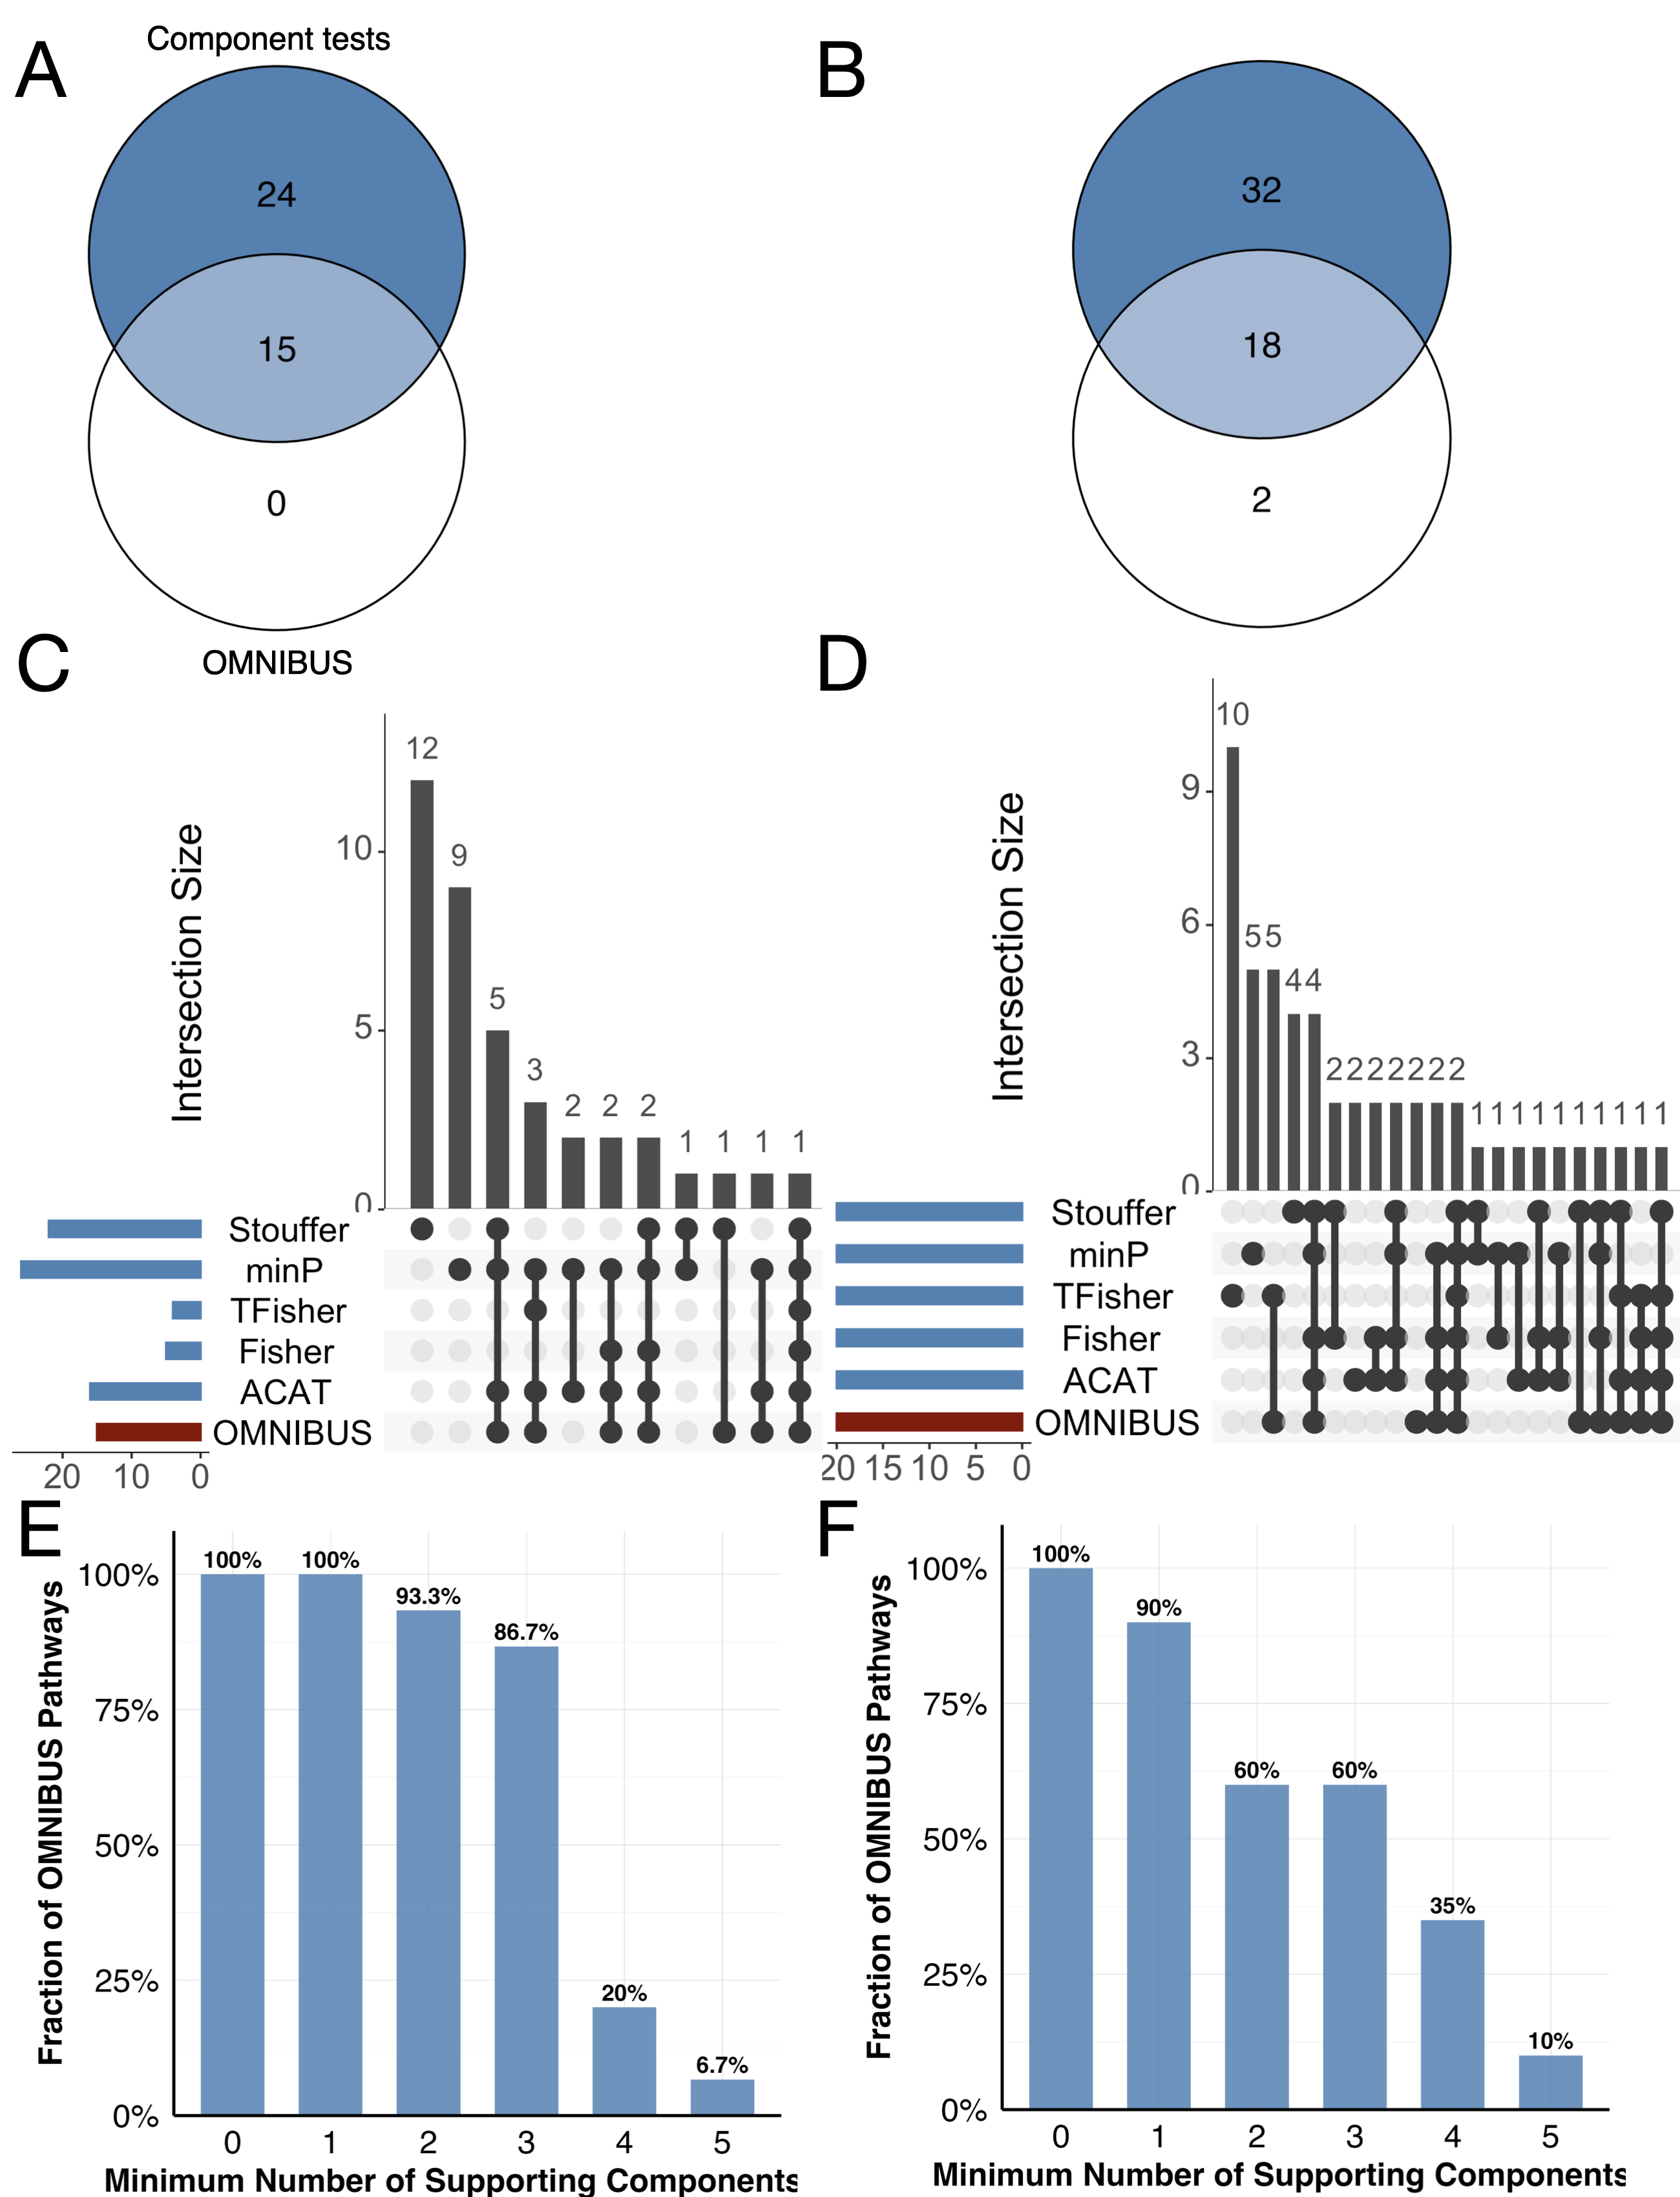
\includegraphics[width=\textwidth]{Figures/Fig6.omni_vs_component_arabidopsis/Fig6.omni_vs_component_arabidopsis.png}
    \caption{\textbf{Omnibus behaves as a broad union, not a narrow intersection.}
    Panels A--B compare the omnibus significant set to the union of component significant sets for \textit{Arabidopsis} (A) and fly (B), demonstrating union-consistency in \textit{Arabidopsis} and a small number of omnibus-only calls in fly, consistent with aggregation of sub-threshold component evidence.
    Panels C--D summarize higher-order intersection structure, showing that omnibus discoveries concentrate in multi-method overlaps while still permitting a limited number of architecture-specific calls.
    Panels E--F quantify multi-component corroboration by plotting the fraction of omnibus pathways supported by at least $k$ component tests, indicating stronger multi-test support in \textit{Arabidopsis} and greater heterogeneity in fly.}
\end{figure*}

We next investigated whether the MVN-calibrated omnibus operates as a true integrator or collapses into an effective surrogate for a single component test. Figure~6A,B indicate that, in \textit{Arabidopsis}, the discovery set identified by the omnibus procedure is fully contained within the union of discoveries from the individual component tests under the same significance threshold (Methods). This demonstrates that the omnibus does not produce unique signals that are decoupled from its constituent evidence layers. By contrast, in \textit{Drosophila}, the omnibus recovers the majority of pathways supported by at least one component test, but additionally identifies a small subset of pathways that are not detected by any single component (Fig.~6B). This behavior illustrates a key strength of the omnibus framework, namely that it can yield statistical significance when multiple component $p$-values are individually suggestive but do not cross the specified threshold on their own. Such omnibus-only hits should not automatically be interpreted as artifacts; rather, they may reflect genuine synergy across component tests and therefore require evaluation under rigorous null calibration. In brief, the \textit{Arabidopsis} omnibus discoveries form a subset of the union of component discoveries, with no omnibus-only calls, whereas in \textit{Drosophila} the omnibus recovers most component-supported pathways plus a small number of additional pathways consistent with evidence aggregation.

Figure~6C,D further show that omnibus-significant pathways are not predominantly driven by calls unique to a single method. Instead, they are enriched for multi-test intersection patterns, indicating that the omnibus preferentially retains pathways that are repeatedly identified across distinct enrichment tests (Fig.~6E,F). In \textit{Arabidopsis}, a substantial proportion of omnibus-significant pathways remains supported even under increasingly stringent multi-test criteria, for example requiring support from at least two or three component methods. By contrast, in the \textit{Drosophila} dataset, multi-test support is generally weaker, with a larger fraction of pathways supported by only one or a small number of component methods. This suggests that the \textit{Arabidopsis} BIO6 signal is more consistently detectable across multiple signal archetypes, whereas the \textit{Drosophila} dataset contains a higher proportion of architecture-specific signals that are detectable only by certain classes of enrichment tests.

Supplementary Figure~5 characterizes the relationship between individual components and the omnibus in more detail. In \textit{Arabidopsis} (Supp.~Fig.~5A), certain components, such as Fisher and TFisher, behave as strict subsets of the omnibus: all pathways identified by these components are also detected by the omnibus, whereas the omnibus additionally recovers pathways not captured by those components. By contrast, other methods, notably minP and Stouffer, exhibit substantial bidirectional non-overlap, indicating that they both contribute unique pathway calls and fail to recover a portion of the pathways identified by the omnibus. In the \textit{Drosophila} dataset (Supp.~Fig.~5B), the overlaps are more evenly distributed across components.

The similarity metrics in Supplementary Figure~5 clarify an important subtlety: the overlap proportion and the Jaccard index answer different questions. The overlap proportion is asymmetric, reflecting how much of a component's discovery set is recovered by the omnibus, whereas the Jaccard index is symmetric, measuring the size of the intersection relative to the union, and therefore penalizes methods that identify many additional pathways beyond the shared set. Consequently, in \textit{Arabidopsis}, cases of high overlap but only moderate Jaccard indicate that a component's calls are largely contained within the omnibus, while the total union remains large because one set contains many additional pathways. In the fly dataset, overlap and Jaccard are more similar in magnitude, implying that component and omnibus discovery set sizes are closer and that the union is less dominated by one method's additional calls. Collectively, Figure~6 and Supplementary Figure~5 support the conclusion that the omnibus is broad in the signal types it can detect, yet selective in what it ultimately reports, behaving as an evidence integrator rather than as a permissive union rule or a disguised single-component test.

\begin{figure*}[!t]
    \centering
    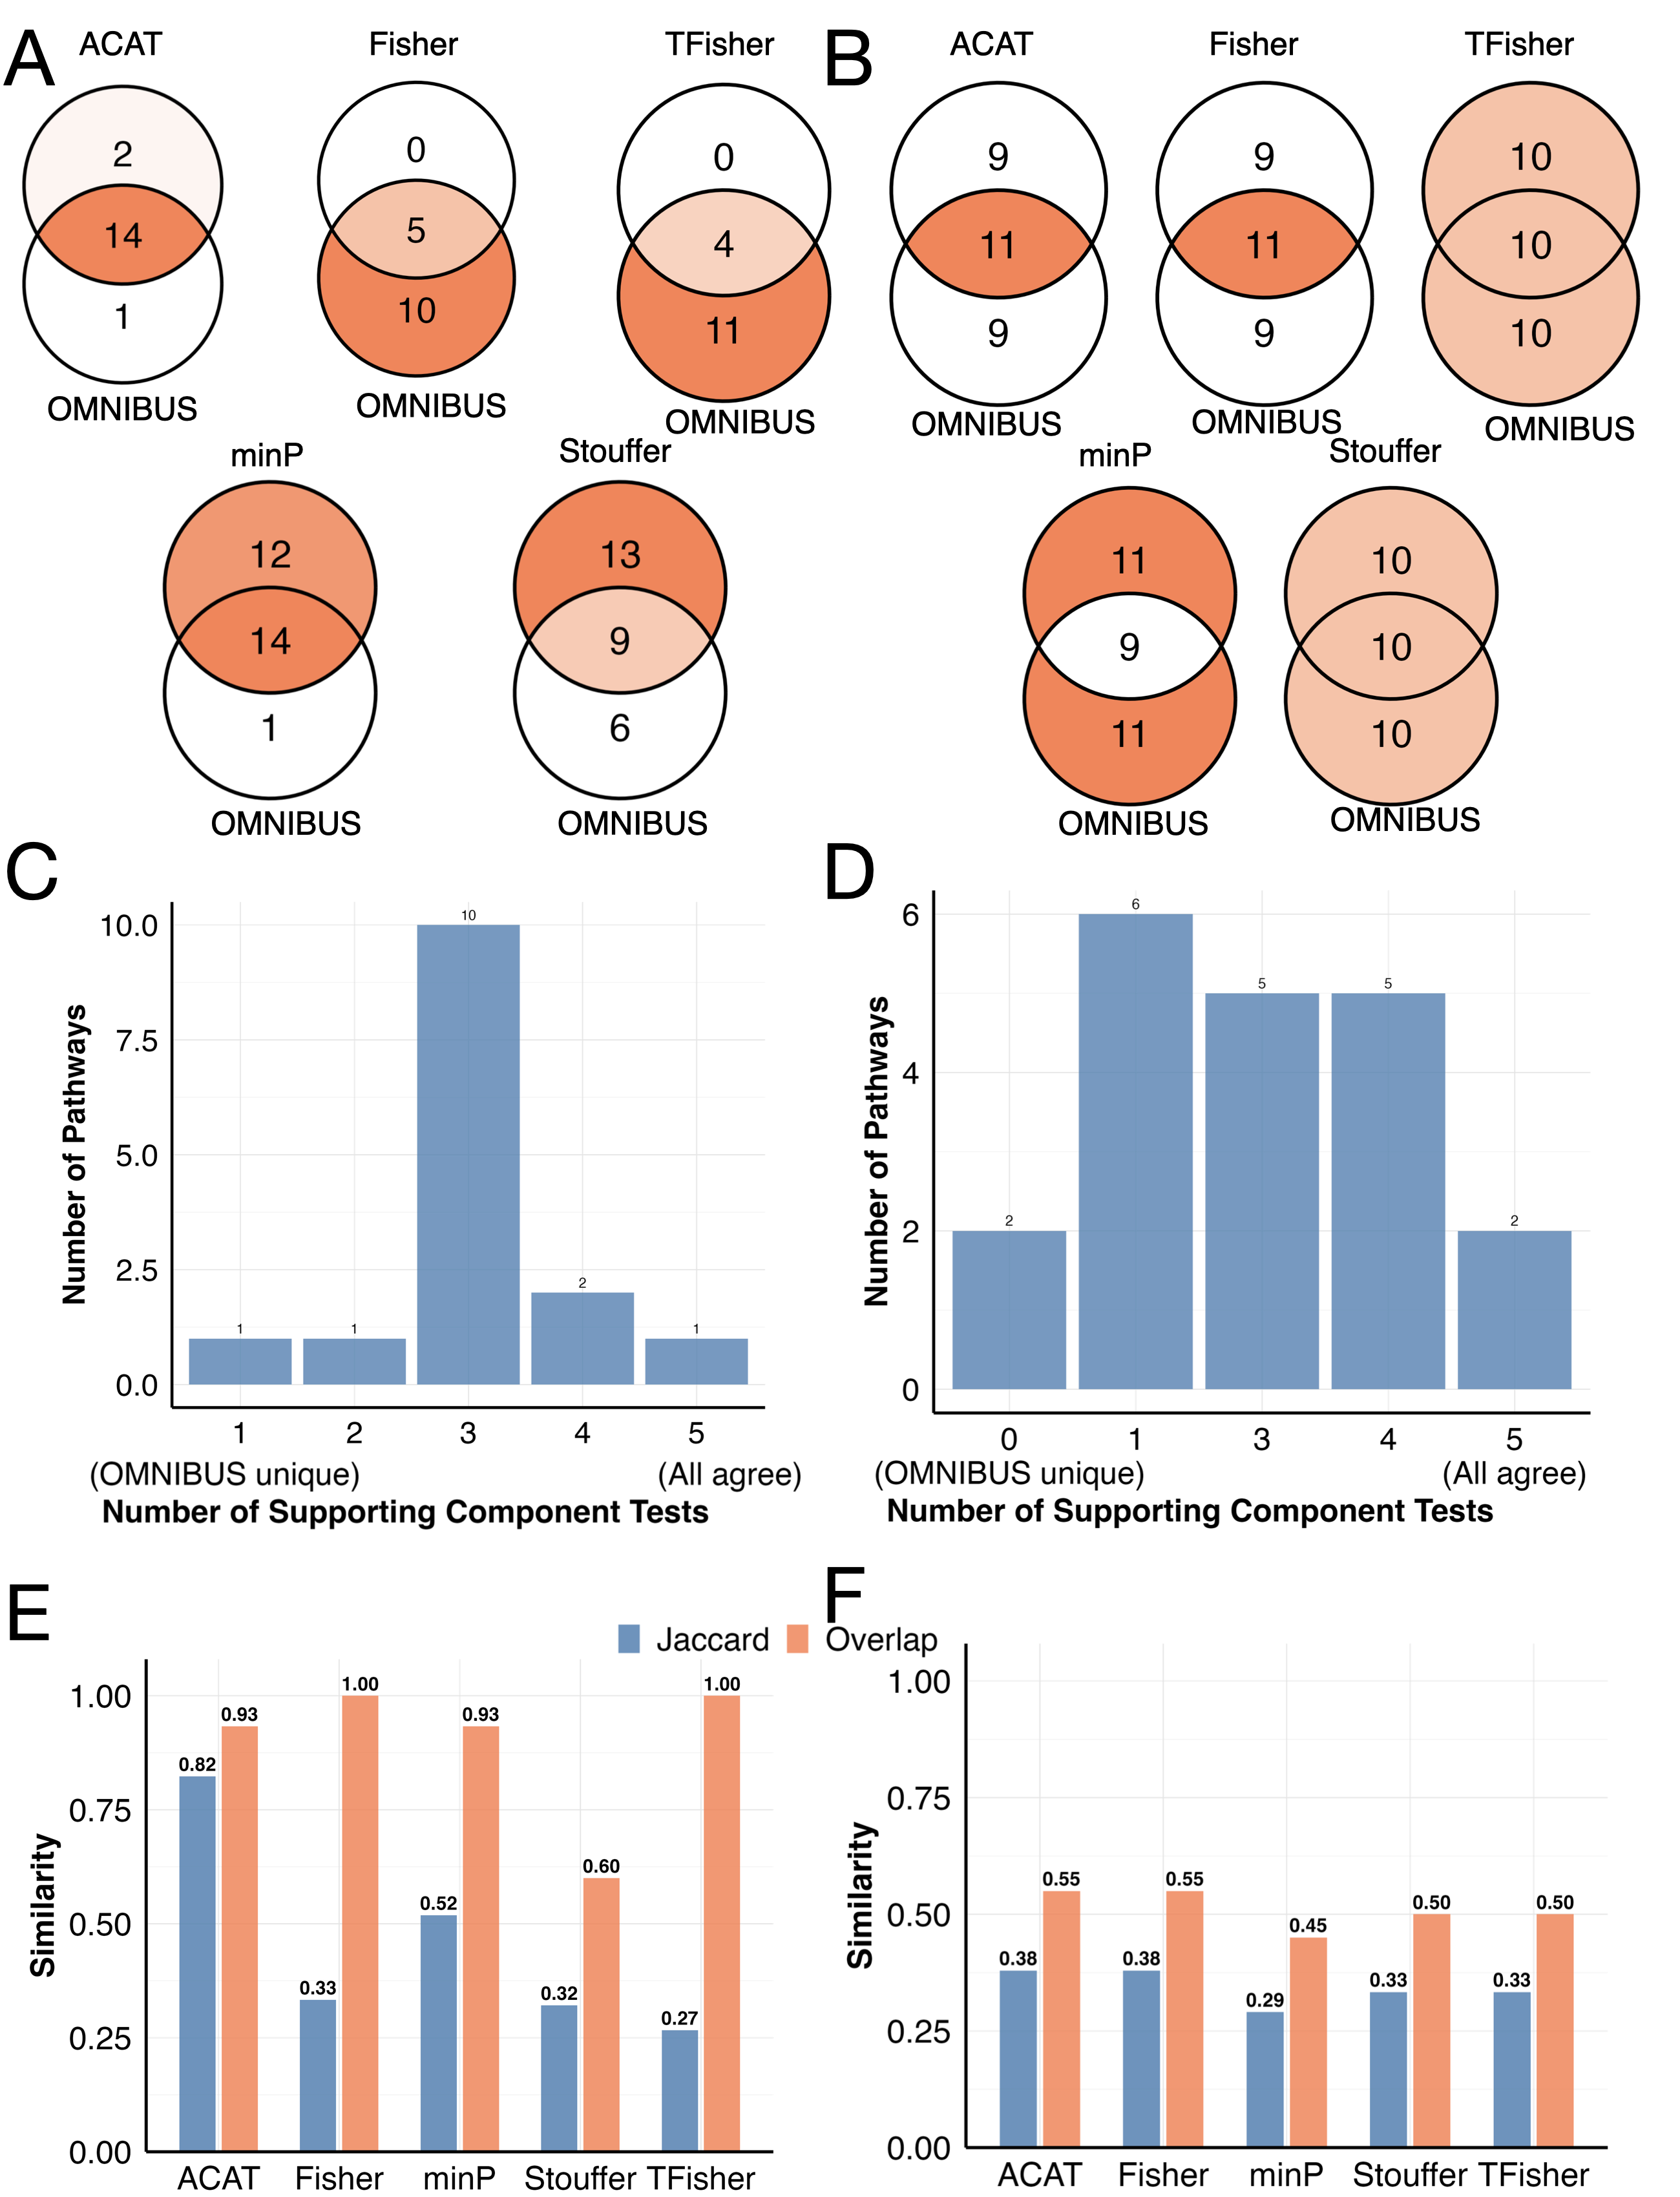
\includegraphics[width=\textwidth]{Figures/SuppFig/SuppFig5.omni_vs_component_arabidopsis.png}
    \caption{\textbf{Component-by-component decomposition of omnibus overlap.}
    Panels A--B show pairwise overlaps between the omnibus and each component test in \textit{Arabidopsis} (A) and fly (B).
    Panels C--D summarize how omnibus-significant pathways distribute across the number of supporting component tests, reinforcing that omnibus calls are enriched for multi-test support but are not identical to any single component.}
\end{figure*}

\subsection{MVN global-null diagnostics support overall calibration}

To verify that differences in discovery patterns reflect power rather than miscalibration, we assessed all component tests and the omnibus under a dependence-preserving global null using multivariate normal (MVN) resampling (Supp.~Fig.~6). The Q--Q plots compare the empirical $p$-value distributions to the theoretical uniform distribution expected under the null hypothesis, while the genomic control factor $\lambda$ provides a scalar summary of global inflation or deflation, with $\lambda \approx 1$ indicating appropriate calibration. Operationally, $\lambda$ captures whether the bulk of null test statistics is globally over- or under-dispersed relative to expectation, whereas empirical type I error directly evaluates threshold-level calibration through the observed rejection rate $\Pr(p < \alpha)$ at a chosen $\alpha$. In both datasets, ACAT, Fisher's method, minP, and Stouffer's method yielded $\lambda$ values close to 1, consistent with well-controlled null behavior under the MVN-based calibration scheme. The omnibus test was likewise close to null in both datasets, slightly conservative in \textit{Arabidopsis} and near 1 in \textit{Drosophila}, which is desirable for a combined procedure intended to maintain stable type I error control across heterogeneous pathway architectures.

The main calibration exception was TFisher in the female fly null diagnostics, which showed a markedly elevated $\lambda$ (Supp.~Fig.~6), indicating a clear departure from the expected null. However, the empirical type I error at $\alpha = 0.05$ remained at or below the nominal level, indicating that TFisher's deviation was not simply a matter of excess false positives at a single threshold. Instead, this pattern is more consistent with a mismatch in null distribution shape or scale that affects the broader $p$-value spectrum without necessarily producing excess rejections at $\alpha = 0.05$. Importantly, the omnibus did not inherit this instability, as both its $\lambda$ and type I error remained close to nominal, consistent with the omnibus functioning as a stabilizing integrator that reduces dependence on the idiosyncratic behavior of any single component test. These diagnostics therefore support the conclusion that the CATFISH MVN framework is approximately nominally calibrated for most individual component tests and for the omnibus statistic, even though a subset of components may still exhibit residual miscalibration.

\begin{figure*}[!t]
    \centering
    \includegraphics[width=\textwidth]{Figures/SuppFig/SuppFig6.null_calibration_combined.png}
    \caption{\textbf{MVN null diagnostics support calibrated inference.}
    Panel A shows Q--Q plots comparing observed versus expected $p$-values under dependence-preserving MVN resampling for each component and the omnibus in \textit{Arabidopsis} and fly.
    Panel B shows genomic control ($\lambda$), summarizing calibration and highlighting elevated $\lambda$ for TFisher in fly while the omnibus remains near 1.
    Panel C shows empirical type I error at $\alpha = 0.05$, confirming near-nominal rejection rates overall and supporting the interpretation that component differences primarily reflect sensitivity to distinct signal architectures rather than systematic false positives.}
\end{figure*}

\subsection{Candidate-gene prioritization integrates GWAS, MAGMA, and pathway evidence}

In Figure~7A,B, we quantified the number of genes supported at each layer under the specified thresholds. For the \textit{Drosophila} analysis, the GWAS evidence layer was deliberately defined using a more permissive significance threshold, reflecting the observation that very few genes satisfy a Bonferroni cutoff. The median number of genes per pathway was lower in \textit{Drosophila} than in \textit{Arabidopsis}. Consequently, pathway membership alone constituted a weaker filtering criterion in the fly analysis.

In \textit{Arabidopsis} (Fig.~7C), a visible subset of genes showed concordant evidence across layers, including support from all three layers, consistent with a mixture of strong locus-driven genes. In fly females (Fig.~7D), many top-ranked genes were supported by GWAS and MAGMA but lacked pathway or top-pathway support at the chosen pathway threshold, consistent with either a smaller or shallower pathway mapping or with pathway-level signals being distributed across many modest genes rather than concentrating on the same top loci that drive GWAS and MAGMA.

Furthermore, genes in the top pathways were enriched for stronger MAGMA signals (Fig.~7E,F), with a clear shift in \textit{Arabidopsis} but a weaker or non-significant shift in fly, indicating that the pathway layer preferentially captures elevated gene-level association in \textit{Arabidopsis}, whereas in fly the enrichment signal is more diffuse.

\begin{figure*}[!t]
    \centering
    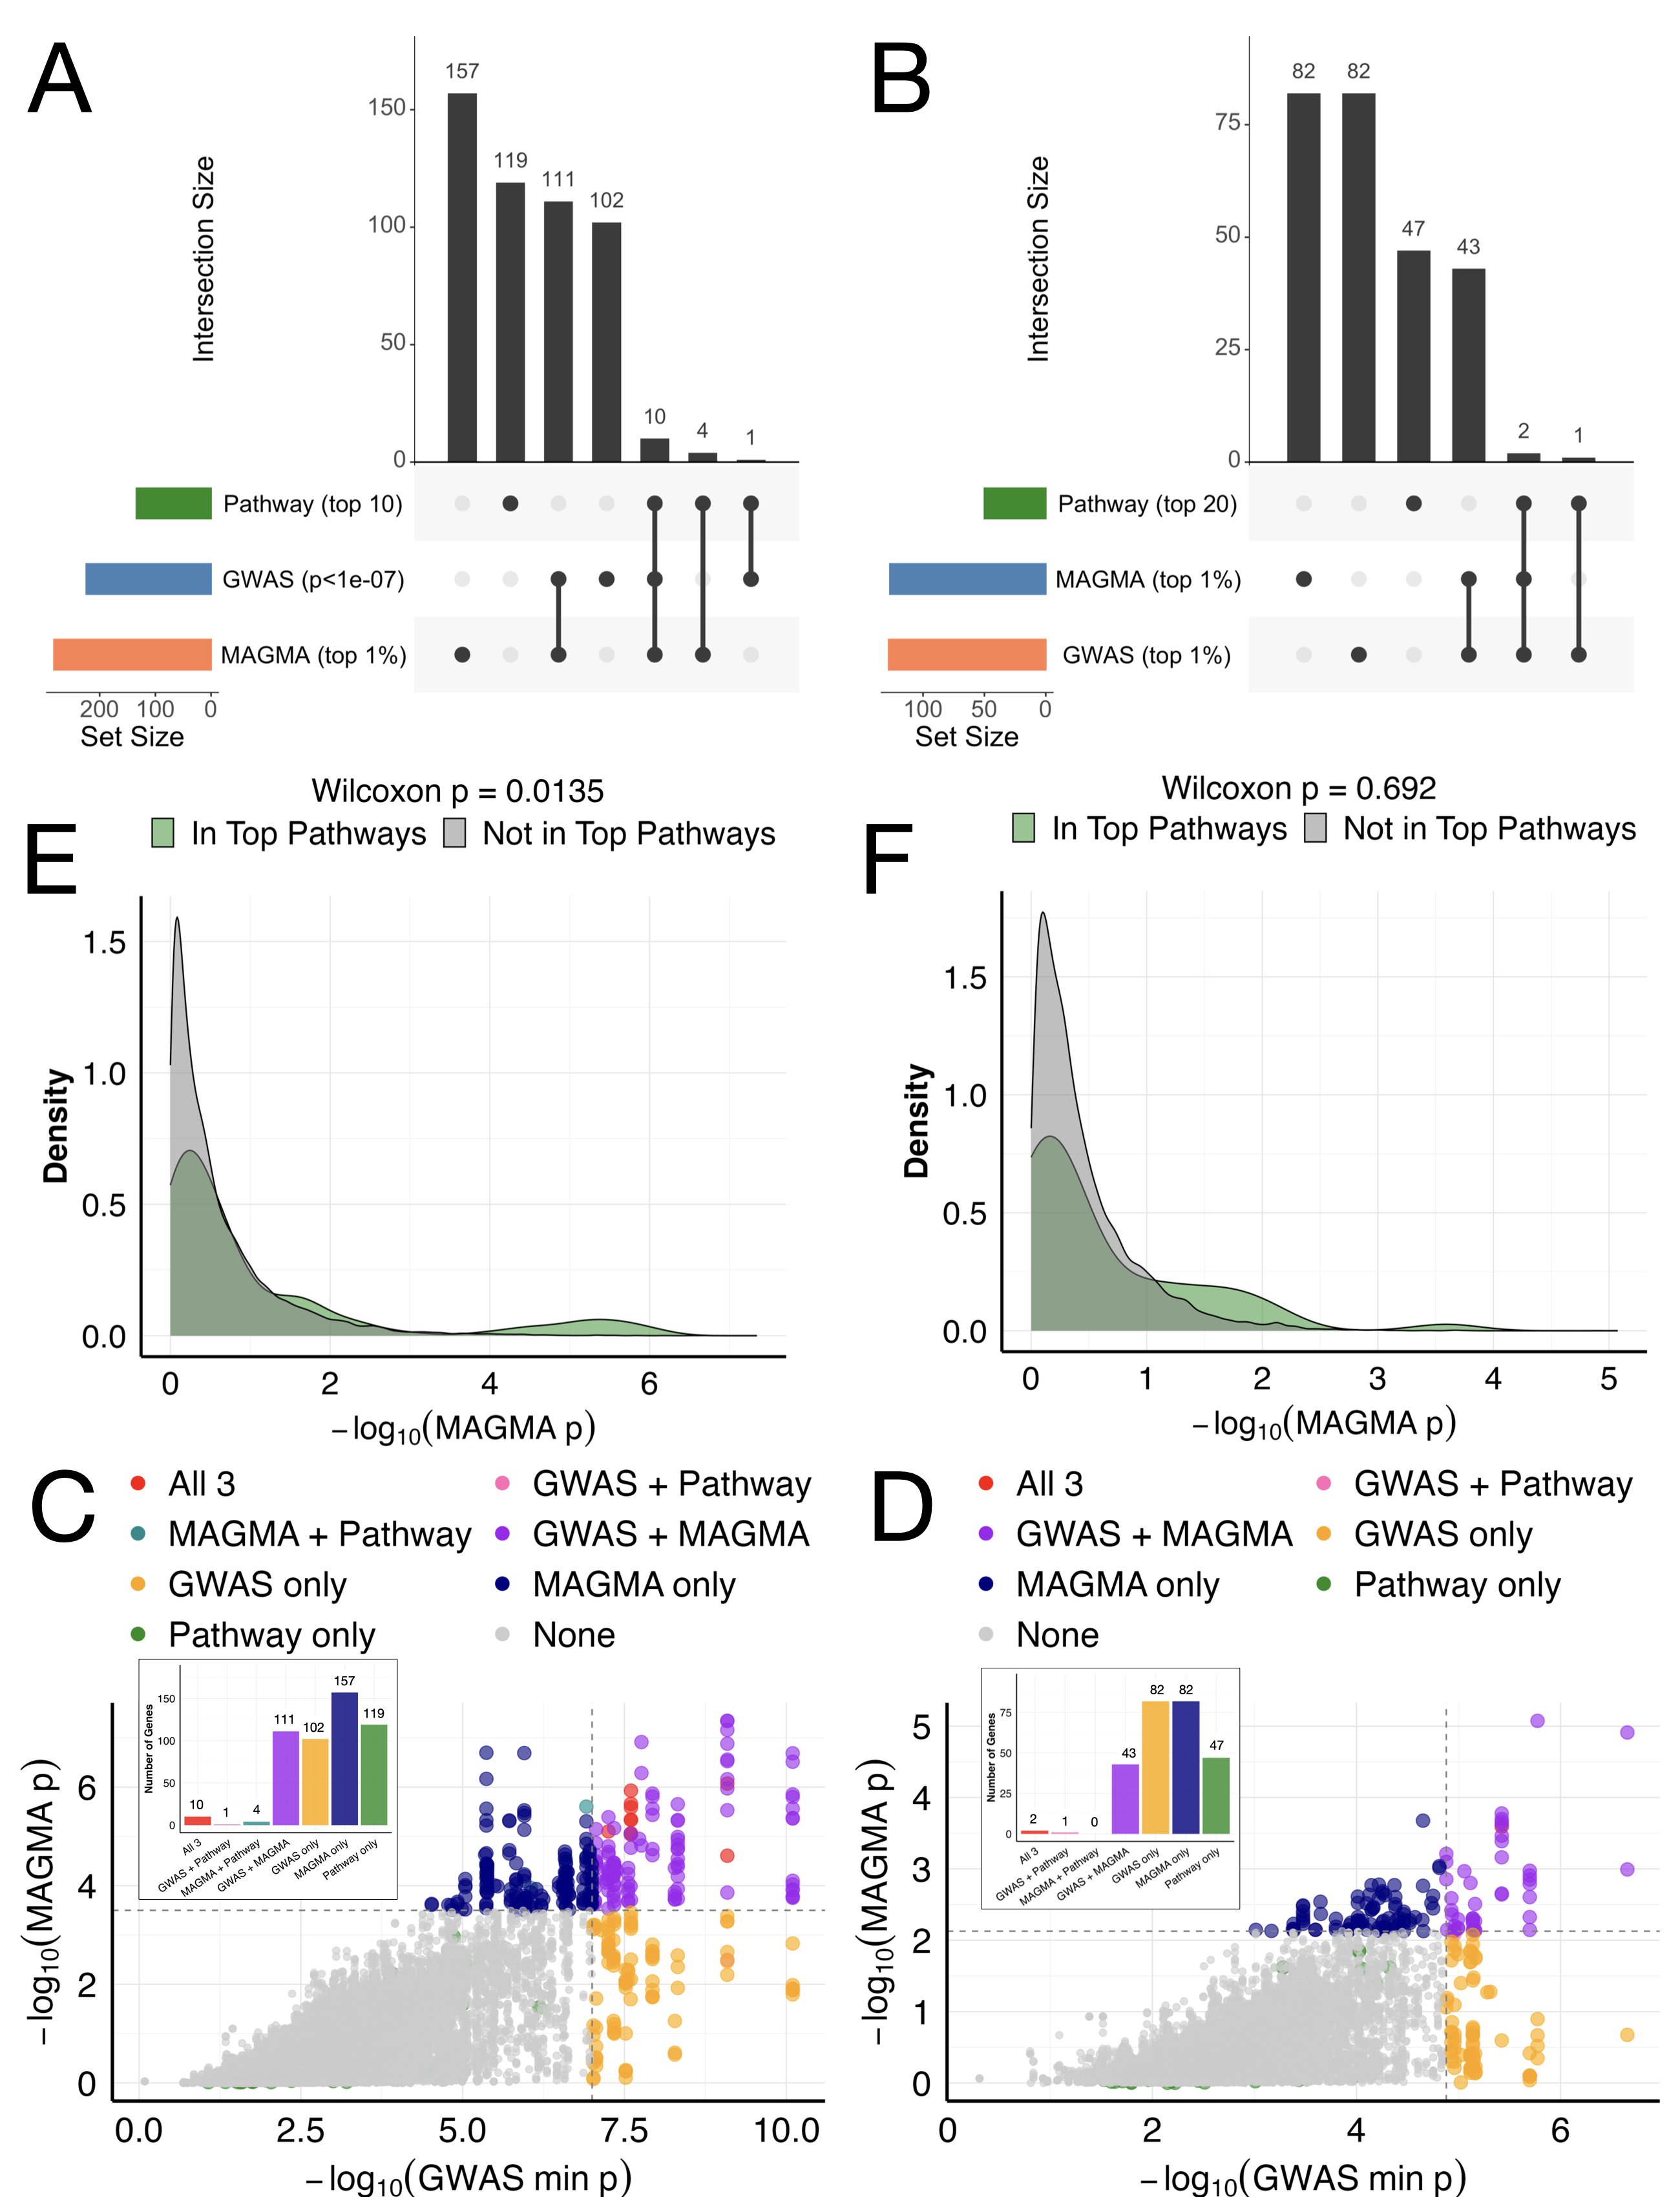
\includegraphics[width=\textwidth]{Figures/Fig7.candidate_gene_analysis_arabidopsis/Fig7.candidate_gene_analysis_arabidopsis.png}
    \caption{\textbf{Multi-layer candidate-gene prioritization integrates GWAS locus evidence, MAGMA gene-level association, and pathway enrichment.}
    Panels A/C/E show \textit{Arabidopsis} (BIO6), and panels B/D/F show female \textit{Drosophila} starvation resistance.
    Panels A--B show UpSet plots summarizing overlap among genes supported by each layer at the thresholds used in the main analysis, namely GWAS-mapped gene support, MAGMA gene-level support, and membership in top enriched pathways (top 10 pathways in \textit{Arabidopsis} and top 20 in fly).
    Panels C--D show gene-level concordance between GWAS and MAGMA. Each point represents a gene, with the x-axis showing GWAS locus evidence mapped to the gene, defined as $-\log_{10}$ of the minimum GWAS $p$-value among mapped variants, and the y-axis showing MAGMA evidence, defined as $-\log_{10}$ of the MAGMA gene-level $p$-value. Points are colored according to which evidence layers support the gene, and inset bar charts report the corresponding counts. Dashed lines indicate the significance cutoffs used to define GWAS- and MAGMA-supported genes.
    Panels E--F show the distribution of MAGMA evidence for genes inside versus outside top enriched pathways; green curves denote genes in top pathways and gray curves denote genes not in top pathways, with Wilcoxon $p$-values testing for a shift toward stronger MAGMA association among pathway genes.}
\end{figure*}

For each gene, \texttt{best\_pathway\_p} denotes the smallest calibrated pathway $p$-value among the top enriched pathways containing that gene (top 10 in \textit{Arabidopsis}; top 20 in fly), and the corresponding pathway identifier is reported as the gene's best-supporting pathway. We further scored candidate genes using a count-based system with continuous evidence strength. Specifically, each gene received a score increment of $+1$ for each evidence layer in which it was supported, namely GWAS, MAGMA, and pathway analysis. In addition, small weighted contributions derived from continuous test statistics were added using $-\log_{10}(p)$ terms, with the MAGMA-derived component assigned a slightly higher weight than the GWAS- and pathway-derived components. This scoring scheme was intentionally designed so that overall ranking is driven primarily by the number of independent evidence layers supporting a gene, while the continuous $-\log_{10}(p)$ contributions serve only to distinguish weakly from strongly supported genes within the same discrete support tier.

In \textit{Arabidopsis}, the top-ranked genes were almost entirely three-layer candidates with strong MAGMA $p$-values and extremely small mapped GWAS $p$-values, and they frequently pointed to a specific best-supporting pathway, for example PWY-5884, a BioCyc pathway identifier corresponding to wax biosynthesis. In female flies, the highest-scoring genes included a smaller set of three-layer candidates with explicit pathway assignments.




\section{Conclusion}

Some Conclusions here.

\section{Conflicts of interest}
The authors declare that they have no competing interests.

\section{Funding}
This work is supported in part by funds from the National Funding Body (NFB: \# XXXXXXX and \# YYYYYYY).

\section{Data availability}
The data underlying this article are available in [repository name, eg, the GenBank Nucleotide Database] at [URL], and can be accessed with [unique identifier, eg, accession number, deposition number].

\section{Author contributions statement}

Must include all authors, identified by initials, for example:
S.R. and D.A. conceived the experiment(s),  S.R. conducted the experiment(s), S.R. and D.A. analysed the results.  S.R. and D.A. wrote and reviewed the manuscript.

\section{Acknowledgments}
The authors thank the anonymous reviewers for their valuable suggestions. This work is supported in part by funds from the National Science Foundation (NSF: \# 1636933 and \# 1920920).


\begin{thebibliography}{12}

\bibitem[Manolio et al.(2009)]{Manolio2009}
Teri~A. Manolio, Francis~S. Collins, Nancy~J. Cox, David~B. Goldstein,
Laura~A. Hindorff, David~J. Hunter, Mark~I. McCarthy, Erin~M. Ramos,
Lon~R. Cardon, Aravinda Chakravarti, and others.
\newblock Finding the missing heritability of complex diseases.
\newblock {\em Nature}, 461(7265):747--753, 2009.

\bibitem[Boyle et al.(2017)]{Boyle2017}
Evan~A. Boyle, Yang~I. Li, and Jonathan~K. Pritchard.
\newblock An expanded view of complex traits: From polygenic to omnigenic.
\newblock {\em Cell}, 169(7):1177--1186, 2017.

\bibitem[Mooney and Wilmot(2015)]{Mooney2015}
Michael~A. Mooney and Brandon Wilmot.
\newblock Gene set analysis: A step-by-step guide.
\newblock {\em American Journal of Medical Genetics Part B: Neuropsychiatric Genetics}, 168(7):517--527, 2015.

\bibitem[de~Leeuw et al.(2015)]{deLeeuw2015}
Christiaan~A. de~Leeuw, Jasper~M. Mooij, Trevor Heskes, and Danielle Posthuma.
\newblock {MAGMA}: Generalized gene-set analysis of {GWAS} data.
\newblock {\em PLoS Computational Biology}, 11(4):e1004219, 2015.

\bibitem[Sherman et al.(2022)]{Sherman2022}
Brad~T. Sherman, Ming Hao, Ju Qiu, Xiaoli Jiao, Michael~W. Baseler,
H.~Clifford Lane, Tomozumi Imamichi, and Weizhong Chang.
\newblock {DAVID}: A web server for functional enrichment analysis and
functional annotation of gene lists (2021 update).
\newblock {\em Nucleic Acids Research}, 50(W1):W216--W221, 2022.

\bibitem[Kolberg et al.(2023)]{Kolberg2023}
Liis Kolberg, Innu Kirsim{\"a}e, Tambet Tamm, Mari Peterson, Kaur Vilo,
Hedi Peterson, and Jaak Vilo.
\newblock g:{P}rofiler---interoperable web service for functional enrichment
analysis and gene identifier mapping (2023 update).
\newblock {\em Nucleic Acids Research}, 51(W1):W207--W212, 2023.

\bibitem[Liao et al.(2019)]{Liao2019}
Yuxing Liao, Jing Wang, Eric~J. Jaehnig, Zhiao Shi, and Bing Zhang.
\newblock {WebGestalt} 2019: Gene set analysis toolkit with revamped {UIs} and
{APIs}.
\newblock {\em Nucleic Acids Research}, 47(W1):W199--W205, 2019.

\bibitem[Subramanian et al.(2005)]{Subramanian2005}
Aravind Subramanian, Pablo Tamayo, Vamsi~K. Mootha, Sayan Mukherjee,
Benjamin~L. Ebert, Michael~A. Gillette, Amanda Paulovich, Scott~L. Pomeroy,
Todd~R. Golub, Eric~S. Lander, and Jill~P. Mesirov.
\newblock Gene set enrichment analysis: A knowledge-based approach for
interpreting genome-wide expression profiles.
\newblock {\em Proceedings of the National Academy of Sciences USA},
102(43):15545--15550, 2005.

\bibitem[Segr{\`e} et al.(2010)]{Segre2010}
Ayellet~V. Segr{\`e}, Leif Groop, Vamsi~K. Mootha, Mark~J. Daly, and
David Altshuler.
\newblock Common inherited variation in mitochondrial genes is not enriched for
type 2 diabetes or related glycemic trait associations.
\newblock {\em PLoS Genetics}, 6(8):e1001058, 2010.

\bibitem[Lee et al.(2012)]{Lee2012}
Phil~H. Lee, Colm O'Dushlaine, Breffni Thomas, and Shaun~M. Purcell.
\newblock {INRICH}: Interval-based enrichment analysis for genome-wide
association studies.
\newblock {\em Bioinformatics}, 28(13):1797--1799, 2012.

\bibitem[Debrabant et al.(2017)]{Debrabant2017}
Birgit Debrabant, Mette Soerensen, Thomas~A. Gerds, and others.
\newblock The null hypothesis of {GSEA}, and a novel statistical model for
competitive gene-set analysis.
\newblock {\em Bioinformatics}, 33(9):1271--1277, 2017.

\bibitem[Geistlinger et al.(2021)]{Geistlinger2021}
Ludwig Geistlinger, Gergely Csaba, Matteo Santarelli, and others.
\newblock Toward a gold standard for benchmarking gene set enrichment analysis.
\newblock {\em Briefings in Bioinformatics}, 22(1):545--556, 2021.

\end{thebibliography}
%%%%%%%%%%%%%%

\begin{appendices}

\section{Bias warning}

Pathway-based analysis for assessing over-representation or enrichment is influenced by various biases, including gene size, pathway size, SNP coverage density, and linkage disequilibrium (LD) patterns, all of which must be addressed explicitly (White et al., 2020; PMC6391732). In CATFISH, we tackle these issues in three phases: (i) The SNP to gene analysis is conducted using MAGMA’s LD-aware multi-SNP model, ensuring that gene-level Z/P values account for local LD structure and SNP density; (ii) we subsequently regress MAGMA gene Z-scores against log(gene length) and log(number of SNPs), utilizing the residual-based $P_adj$ for all subsequent gene to pathway analyses, thereby eliminating any remaining dependence on gene size and SNP density; and (iii) at the pathway level, we avoid simplistic over-representation tests, opting instead to calibrate our omnibus statistics through gene-label LD-aware permutations that maintain each gene’s adjusted $p$-value and the observed distribution of pathway sizes, yielding enrichment $p$-values that are resilient to these established biases.

Link: https://pmc.ncbi.nlm.nih.gov/articles/PMC6391732/

\section{Mathematical details of CATFISH}\label{app:catfish_math}

\subsection{Extended notation}

For a pathway (gene set) $S$, let $G = |S|$ denote the number of genes in the pathway. For each gene $g \in S$, let $p_g$ denote the gene-level association $p$-value and let $Z_g$ denote the corresponding gene-level $Z$ statistic when available. We collect these into pathway-level vectors
\[
\mathbf{p}_S = (p_1, p_2, \dots, p_G),
\qquad
\mathbf{Z}_S = (Z_1, Z_2, \dots, Z_G).
\]

When gene-level adjustment is applied, we denote the adjusted quantities by
\[
\mathbf{p}_{S,\mathrm{adj}} = (p_{1,\mathrm{adj}}, \dots, p_{G,\mathrm{adj}}),
\qquad
\mathbf{Z}_{S,\mathrm{adj}} = (Z_{1,\mathrm{adj}}, \dots, Z_{G,\mathrm{adj}}).
\]

Unless otherwise stated, definitions below are written using the unadjusted inputs.

\subsection{Gene-level association statistics}

Gene-level association evidence was derived from MAGMA, which aggregates SNP-level association signals within each gene while accounting for local LD using an external reference panel. We used MAGMA's SNP-wise gene model, which combines information from both mean-like and top-SNP-like within-gene architectures to generate a unified gene-level association summary. The resulting MAGMA outputs, including gene-level $p$-values and gene-level $Z$ statistics, served as the common input to all downstream CATFISH pathway analyses.

\subsection{Gene-level adjustment for gene size and SNP density}

To reduce residual dependence of gene-level signal on gene size and SNP density, we optionally regressed the MAGMA gene-level $Z$ statistic on gene-level covariates. Let $L_g$ denote gene length and $S_g$ denote the number of SNPs mapped to gene $g$. We fit
\[
Z_g = \beta_0 + \beta_1 \log(L_g) + \beta_2 \log(S_g) + \varepsilon_g.
\]

We then define the adjusted residual score as
\[
Z_g^{\mathrm{adj}} = Z_g - \widehat{Z}_g,
\qquad
\widehat{Z}_g = \widehat{\beta}_0 + \widehat{\beta}_1 \log(L_g) + \widehat{\beta}_2 \log(S_g),
\]
and the corresponding adjusted two-sided $p$-value as
\[
p_{g,\mathrm{adj}} = 2\Phi\!\left(-\left|Z_g^{\mathrm{adj}}\right|\right),
\]
where $\Phi(\cdot)$ is the standard normal cumulative distribution function.

\subsection{Pathway-level component statistics}

Because all pathway statistics are computed from the same within-pathway gene-level evidence, the component tests are mutually dependent. Independence-based reference nulls are therefore used only as analytic definitions. Final inferential calibration is obtained through the unified dependence-aware null framework described below.

\subsubsection{ACAT}

For each gene,
\[
t_g = \tan\left(\pi\left(\tfrac{1}{2} - p_g\right)\right).
\]
With nonnegative weights $w_g$ such that $\sum_{g \in S} w_g = 1$, the pathway-level ACAT statistic is
\[
T_{\mathrm{ACAT}}(S)
=
\sum_{g \in S} w_g \tan\left(\pi\left(\tfrac{1}{2} - p_g\right)\right),
\]
with corresponding analytic combined $p$-value
\[
p_{\mathrm{ACAT}}(S)
=
\tfrac{1}{2} - \frac{1}{\pi}\arctan\left(T_{\mathrm{ACAT}}(S)\right).
\]

\subsubsection{Fisher's method}

Fisher's pathway statistic is
\[
T_{\mathrm{Fisher}}(S) = -2\sum_{g \in S}\log(p_g).
\]
Under independence,
\[
T_{\mathrm{Fisher}}(S) \sim \chi^2_{2G},
\]
which yields the standard analytic Fisher $p$-value.

\subsubsection{Adaptive soft TFisher}

For a given soft threshold $\tau \in (0,1]$, the soft TFisher statistic is
\[
W^{\mathrm{soft}}(S;\tau)
=
\sum_{g \in S}
\left[-2\log(p_g) + 2\log(\tau)\right]_+,
\qquad
(x)_+ = \max(x,0).
\]

CATFISH evaluates this statistic across a fixed threshold grid
\[
\mathcal{T} = \{0.20, 0.10, 0.05, 0.01\},
\]
and defines the adaptive TFisher component as the minimum calibrated TFisher $p$-value across $\tau \in \mathcal{T}$.

\subsubsection{Stouffer's method}

For a pathway with $G$ genes, the default unweighted Stouffer statistic is
\[
Z_{\mathrm{Stouffer}}(S)
=
\frac{1}{\sqrt{G}}\sum_{g \in S} Z_g,
\]
with one-sided analytic $p$-value
\[
p_{\mathrm{Stouffer}}(S) = 1 - \Phi\!\left(Z_{\mathrm{Stouffer}}(S)\right).
\]

If nonnegative weights $w_g$ are supplied, the weighted version is
\[
Z_{\mathrm{Stouffer}}^{(w)}(S)
=
\frac{\sum_{g \in S} w_g Z_g}{\sqrt{\sum_{g \in S} w_g^2}}.
\]

\subsubsection{minP}

The minP statistic is defined as
\[
T_{\min}(S) = \min_{g \in S} p_g.
\]
Under independence, its canonical Tippett/\v{S}id\'ak mapping is
\[
p_{\mathrm{minP}}(S)
=
1 - \left(1 - T_{\min}(S)\right)^G.
\]

\subsection{Sources of dependence}

Dependence in CATFISH arises at two levels. First, the component pathway tests are deterministically coupled because they are all computed from the same within-pathway gene-level evidence, namely $\{p_g\}_{g \in S}$ and, when used, $\{Z_g\}_{g \in S}$. Consequently, the resulting component pathway $p$-values are correlated even if the genes themselves were independent. For example, Fisher's method and soft TFisher both respond to an excess of moderately small gene-level $p$-values, Stouffer's method is driven by coherent shifts in gene-level $Z$ scores, and ACAT and minP both become extreme when one or a few genes have exceptionally small $p$-values.

Second, gene-level inputs within a pathway may themselves be correlated due to LD, overlapping SNP mappings, shared genomic structure, or broader polygenic background effects. This additional gene--gene dependence compounds the deterministic coupling among component tests. Post hoc selection across methods, such as taking the minimum across methods or adaptively selecting the TFisher threshold, further increases dependence among reported statistics. Consequently, analytic across-method combinations that assume independence may be miscalibrated, motivating the dependence-aware null calibration framework described below.

\subsection{Numerical safeguards}

To avoid numerical instability in $\log(\cdot)$ and Cauchy transforms, gene-level $p$-values are clipped to
\[
p_g \leftarrow \min\{1-p_{\min}, \max(p_g, p_{\min})\},
\qquad p_{\min}=10^{-15}.
\]

If a gene appears multiple times in a pathway definition, duplicate entries are collapsed prior to pathway analysis so that each gene contributes only once. When duplicate gene entries occur, the retained gene-level value is the minimum observed $p$-value for that gene.

\subsection{Omnibus pathway combination across methods}

Let the available component pathway $p$-values for pathway $S$ be
\[
\mathcal{P}(S)
=
\left\{
p_{\mathrm{ACAT}}(S),\,
p_{\mathrm{Fisher}}(S),\,
p_{\mathrm{TFisher}}(S),\,
p_{\mathrm{minP}}(S),\,
p_{\mathrm{Stouffer}}(S)
\right\},
\]
with $K = |\mathcal{P}(S)| \le 5$ depending on whether Stouffer is available.

\subsubsection{ACAT-O}

With method-level weights $v_j \ge 0$ satisfying $\sum_{j=1}^{K} v_j = 1$, the across-method ACAT omnibus is
\[
T_{\mathrm{omni,ACAT}}(S)
=
\sum_{j=1}^{K} v_j \tan\!\bigl(\pi(0.5-p_j)\bigr),
\]
and
\[
p_{\mathrm{omni,ACAT}}(S)
=
0.5-\frac{1}{\pi}\arctan\!\bigl(T_{\mathrm{omni,ACAT}}(S)\bigr).
\]

\subsubsection{minP-O}

The across-method minimum is
\[
T_{\mathrm{omni,min}}(S)=\min_{j=1,\dots,K} p_j(S),
\]
with analytic independence-based mapping
\[
p_{\mathrm{omni,min}}(S)
=
1-\bigl(1-T_{\mathrm{omni,min}}(S)\bigr)^K.
\]

\subsection{Dependence-aware null calibration}

Because both gene-level inputs and across-method component tests are dependent, CATFISH calibrates the omnibus under a null generator that preserves this dependence. Two complementary null-generation strategies are supported: global gene-set resampling and LD-aware MVN calibration. The former preserves the empirical genome-wide marginal distribution of gene-level evidence and cross-method coupling but is LD-agnostic within a pathway. The latter explicitly preserves within-pathway gene--gene dependence and is the recommended inferential procedure.

\subsubsection{Global resampling}

In the global resampling mode, a null pathway of size $d$ is generated by sampling $d$ genes from a genome-wide pool of genes with valid MAGMA outputs. Each sampled gene contributes its paired evidence $(p_g, Z_g)$ when $Z_g$ is available, ensuring that both $p$-based and $Z$-based component tests are recomputed from the same resampled gene set in each null replicate. For replicate $b$, CATFISH recalculates all component pathway statistics on the resampled pathway and applies the same omnibus operator used for the observed data.

Formally, let $\mathcal{G}$ denote the genome-wide pool of genes with valid pathway inputs, and let pathway $S$ have size $|S|=d$. For each replicate $b=1,\dots,B$, CATFISH samples $d$ genes from $\mathcal{G}$, typically without replacement when $d \le |\mathcal{G}|$, and constructs a null pathway-level evidence set
\[
\mathbf{p}^{(b)}_{\mathrm{global}}(S), \qquad \mathbf{Z}^{(b)}_{\mathrm{global}}(S).
\]
All component tests are recomputed on this resampled pathway, yielding replicate component $p$-values $\{p_j^{(b)}(S)\}$, and the omnibus operator is then applied:
\[
p_{\mathrm{omni}}^{(b)}(S)
=
\mathcal{O}\!\left(\{p_j^{(b)}(S)\}\right).
\]

If $p_{\mathrm{omni}}^{\mathrm{obs}}(S)$ denotes the observed omnibus value, the globally resampled omnibus $p$-value is estimated as
\[
\hat p_{\mathrm{omni,global}}(S)
=
\frac{
1+\sum_{b=1}^{B}\mathbf{1}\!\left(
p_{\mathrm{omni}}^{(b)}(S)\le p_{\mathrm{omni}}^{\mathrm{obs}}(S)
\right)
}{
B+1
}.
\]

This approach preserves the empirical genome-wide marginal distribution of gene-level evidence and captures cross-method coupling because all component tests are recomputed from the same sampled gene set. However, it does not preserve pathway-specific LD structure and is therefore treated as a secondary calibration mode relative to the LD-aware MVN procedure.


\begin{algorithm}[htbp]
\caption{Global gene-set resampling calibration for pathway $S$}
\label{alg:global_resampling}
\begin{algorithmic}[1]
\Require Pathway $S$ of size $d$, global gene pool $\mathcal{G}$, observed gene-level inputs $\{(p_g, Z_g)\}$, number of resamples $B$, omnibus operator $f_{\mathrm{omni}}$
\Ensure Calibrated omnibus $p$-value $\hat p_{\mathrm{omni,global}}(S)$

\State Construct the global gene pool $\mathcal{G}$ from all genes with valid pathway inputs
\State Align gene-level $p$-values and $Z$-scores so that each gene contributes a paired record $(p_g, Z_g)$
\State Compute the observed component pathway $p$-values for $S$
\State Compute the observed omnibus value
\[
p_{\mathrm{omni}}^{\mathrm{obs}}(S)=
f_{\mathrm{omni}}\!\left(\{p_j^{\mathrm{obs}}(S)\}\right)
\]

\For{$b=1,\dots,B$}
    \State Sample $d$ genes uniformly from $\mathcal{G}$ to obtain index set
    \[
    I^{(b)}=(i_1,\dots,i_d)
    \]
    \State Construct null pathway evidence
    \[
    P^{(b)}=(P_{i_1},\dots,P_{i_d}),
    \qquad
    Z^{(b)}=(Z_{i_1},\dots,Z_{i_d})
    \]
    \State Recompute all component tests on the same sampled gene set:
    \State \hspace{1em} ACAT from $P^{(b)}$
    \State \hspace{1em} Fisher from $P^{(b)}$
    \State \hspace{1em} TFisher from $P^{(b)}$ over the same $\tau$ grid
    \State \hspace{1em} minP from $P^{(b)}$
    \State \hspace{1em} Stouffer from $Z^{(b)}$
    \State Combine replicate component $p$-values using the same omnibus rule:
    \[
    p_{\mathrm{omni}}^{(b)}(S)
    =
    f_{\mathrm{omni}}\!\left(\{p_j^{(b)}(S)\}\right)
    \]
\EndFor

\State Estimate the calibrated omnibus $p$-value as
\[
\hat p_{\mathrm{omni,global}}(S)
=
\frac{
1+\sum_{b=1}^{B}\mathbf{1}\!\left(
p_{\mathrm{omni}}^{(b)}(S)\le p_{\mathrm{omni}}^{\mathrm{obs}}(S)
\right)
}{
B+1
}
\]

\State \Return $\hat p_{\mathrm{omni,global}}(S)$
\end{algorithmic}
\end{algorithm}



\subsubsection{LD-aware MVN calibration}

In the LD-aware mode, CATFISH constructs a pathway-specific gene--gene correlation matrix $R_S$ and generates null gene-level score vectors as
\[
Z^{(b)} \sim \mathcal{N}(0, R_S),
\qquad b=1,\dots,B.
\]
Here, $R_S$ is treated as fixed for a given pathway and encodes the expected dependence among gene-level statistics under the null. The MVN procedure does not resample the correlation matrix itself; rather, it repeatedly generates new null gene-score vectors whose joint covariance structure is determined by $R_S$.

\paragraph{Construction of the pathway-specific correlation matrix.}
For each pathway $S=\{g_1,\dots,g_d\}$, the pathway-specific gene--gene correlation matrix $R_S$ is constructed from pairwise gene-correlation estimates, typically obtained from MAGMA output. Diagonal entries are set to 1, and off-diagonal entries are filled using the available pairwise correlations for genes within the pathway. When a gene pair is missing from the pairwise correlation output, the corresponding entry is set to 0 by default. This missing-as-zero convention corresponds to assuming independence for unobserved gene pairs while retaining the observed correlation structure.

Formally, if $r_{ij}$ denotes the available pairwise correlation between genes $g_i$ and $g_j$, then
\[
(R_S)_{ii}=1,
\qquad
(R_S)_{ij}=
\begin{cases}
r_{ij}, & \text{if the pairwise estimate is available,} \\
0, & \text{otherwise.}
\end{cases}
\]

\paragraph{Numerical stabilization of the MVN null.}
Because estimated pathway-specific correlation matrices may be ill-conditioned or only approximately positive definite, CATFISH applies numerical stabilization before MVN simulation when necessary. In practice, this may include clipping extreme correlations, for example $|r_{ij}|\le 0.999$, replacing missing entries with 0 as above, and applying a nearest positive-definite correction or a small diagonal jitter. These steps improve numerical robustness of MVN simulation without changing the overall interpretation of the LD-aware null.

\paragraph{Generation of correlated null gene-level scores.}
To simulate from the pathway-specific null, CATFISH factorizes the stabilized matrix $R_S$ as
\[
R_S = LL^\top,
\]
where $L$ is a lower-triangular matrix, for example obtained by a Cholesky decomposition when $R_S$ is positive definite. Let
\[
u^{(b)} \sim \mathcal{N}(0, I_d)
\]
denote a vector of independent standard normal draws of length $d$, where $I_d$ is the $d\times d$ identity matrix. CATFISH then forms the correlated null gene-score vector as
\[
Z^{(b)} = L u^{(b)}.
\]
By construction,
\[
\mathrm{Cov}\!\left(Z^{(b)}\right)
=
L\,\mathrm{Cov}\!\left(u^{(b)}\right)L^\top
=
L I_d L^\top
=
LL^\top
=
R_S.
\]
Thus, the simulated null scores are random, but not independent: genes with high pairwise correlation in $R_S$ tend to co-vary across null replicates, whereas genes with near-zero correlation vary more independently. This preserves the gene-level dependence structure induced by LD in the pathway-specific null model.

\paragraph{Gaussian-copula mapping to gene-level $p$-values.}
For $p$-based component tests, null gene-level $p$-values are derived from the same latent MVN draw using a Gaussian copula:
\[
U_g^{(b)} = \Phi\!\left(Z_g^{(b)}\right),
\qquad
p_g^{(b)} = 2\min\{U_g^{(b)}, 1-U_g^{(b)}\}.
\]
This preserves dependence across genes while ensuring coherent null inputs across both $Z$-based and $p$-based component statistics. If a one-sided gene-level convention is used instead, the mapping may be written as
\[
p_g^{(b)} = 1-\Phi\!\left(Z_g^{(b)}\right),
\]
with the direction chosen appropriately.

\paragraph{Component recomputation and omnibus calibration.}
For each replicate, CATFISH computes the replicate component vector
\[
\mathbf{p}^{(b)}(S)
=
\big(
p_{\mathrm{ACAT}}^{(b)}(S),\,
p_{\mathrm{Fisher}}^{(b)}(S),\,
p_{\mathrm{TFisher}}^{(b)}(S),\,
p_{\mathrm{Stouffer}}^{(b)}(S),\,
p_{\mathrm{minP}}^{(b)}(S)
\big),
\]
and then applies the omnibus operator
\[
p_{\mathrm{omni}}^{(b)}(S)=\mathcal{O}\!\left(\mathbf{p}^{(b)}(S)\right).
\]

If $p_{\mathrm{omni}}^{\mathrm{obs}}(S)$ denotes the observed omnibus value from the real pathway data, the calibrated omnibus $p$-value is
\[
\hat p_{\mathrm{omni,mvn}}(S)
=
\frac{
1+\sum_{b=1}^{B}\mathbf{1}\!\left(
p_{\mathrm{omni}}^{(b)}(S)\le p_{\mathrm{omni}}^{\mathrm{obs}}(S)
\right)
}{
B+1
}.
\]

This unified calibration targets the null distribution of the full pathway-analysis procedure by recomputing every component test and the omnibus operator under the same dependence-preserving null draw. Because all component statistics are recalculated from the same simulated pathway, the MVN procedure preserves both within-pathway gene dependence and cross-method dependence by construction. In particular, CATFISH does not separately calibrate each component and then recalibrate the omnibus a second time for primary inference; rather, the recommended inferential quantity is the omnibus statistic calibrated directly under the full MVN null pipeline.

\subsection{MVN calibration of component statistics}

CATFISH can optionally report MVN-calibrated component $p$-values for diagnostic purposes. For a given component $j$, its MVN-calibrated value is
\[
\hat p_j(S)
=
\frac{
1+\sum_{b=1}^{B}\mathbf{1}\!\left(
p_j^{(b)}(S)\le p_j^{\mathrm{obs}}(S)
\right)
}{
B+1
}.
\]

These component-wise calibrated values are useful descriptively, but they remain dependent across methods and are not treated as independent inferential quantities unless the entire downstream combination procedure is itself recalibrated. Because all component-wise calibrated values are obtained from the same set of null replicates and are computed from the same underlying pathway evidence, they remain jointly dependent even after marginal calibration to the unit interval. Accordingly, CATFISH uses direct MVN calibration of the final omnibus statistic as the primary LD-aware inferential procedure.

\subsection{Choice of final omnibus \texorpdfstring{$p$}{p}-value}

Depending on the calibration mode, CATFISH may report an analytic omnibus, a globally resampled omnibus, or an MVN-calibrated omnibus. The final pathway-level omnibus is chosen as
\[
p_{\mathrm{omni,final}}(S)=
\begin{cases}
\hat p_{\mathrm{omni,mvn}}(S), & \text{if MVN calibration is performed,} \\
\hat p_{\mathrm{omni,global}}(S), & \text{otherwise if global calibration is performed,} \\
p_{\mathrm{omni,analytic}}(S), & \text{otherwise.}
\end{cases}
\]

\subsection{Default implementation choices}

Unless otherwise stated, CATFISH uses equal weights within ACAT and ACAT-O, an adaptive soft-TFisher threshold grid $\mathcal{T}=\{0.20, 0.10, 0.05, 0.01\}$, one-sided Stouffer aggregation for MAGMA association-strength $Z$ scores, clipping of gene-level $p$-values at $p_{\min}=10^{-15}$, and LD-aware MVN calibration as the primary inferential mode. Missing pairwise gene correlations are set to 0 when constructing pathway-specific correlation matrices, with numerical stabilization applied as needed to ensure positive-definite MVN simulation.

\section{Candidate-gene prioritization score}\label{app:candidate_score}

To prioritize genes supported across multiple analytical layers, we combined evidence from GWAS locus support, MAGMA gene-level significance, and pathway-level enrichment. For each gene $g$, the composite score was defined as
\[
\mathrm{score}(g)
=
\mathbf{1}\{\mathrm{GWAS}\}
+
\mathbf{1}\{\mathrm{MAGMA}\}
+
\mathbf{1}\{\mathrm{PATH}\}
+
0.2\cdot\left[-\log_{10}\!\left(p_{\mathrm{MAGMA}}\right)\right]
+
0.1\cdot\left[-\log_{10}\!\left(p_{\mathrm{GWAS}}\right)\right]
+
0.1\cdot\left[-\log_{10}\!\left(p_{\mathrm{PATH}}\right)\right].
\]

This formulation gives primary weight to agreement across discrete evidence layers while allowing modest within-layer ranking by continuous signal strength. Genes supported by at least two layers were prioritized for downstream interpretation.

\end{appendices}

\end{document}
